%%%%%%%%%%%%%%%%%%%%%%%%%%%%%%%%%%%%%%%%%%%%%%%%%%%%%%%%%%%%%%%
%% OXFORD THESIS TEMPLATE

% Use this template to produce a standard thesis that meets the Oxford University requirements for DPhil submission
%
% Originally by Keith A. Gillow (gillow@maths.ox.ac.uk), 1997
% Modified by Sam Evans (sam@samuelevansresearch.org), 2007
% Modified by John McManigle (john@oxfordechoes.com), 2015
%
% This version Copyright (c) 2015-2023 John McManigle
%
% Broad permissions are granted to use, modify, and distribute this software
% as specified in the MIT License included in this distribution's LICENSE file.
%

% I've (John) tried to comment this file extensively, so read through it to see how to use the various options.  Remember
% that in LaTeX, any line starting with a % is NOT executed.  Several places below, you have a choice of which line to use
% out of multiple options (eg draft vs final, for PDF vs for binding, etc.)  When you pick one, add a % to the beginning of
% the lines you don't want.


%%%%% CHOOSE PAGE LAYOUT
% The most common choices should be below.  You can also do other things, like replacing "a4paper" with "letterpaper", etc.

% This one will format for two-sided binding (ie left and right pages have mirror margins; blank pages inserted where needed):
%\documentclass[a4paper,twoside]{ociamthesis}
% This one will format for one-sided binding (ie left margin > right margin; no extra blank pages):
%\documentclass[a4paper]{ociamthesis}
% This one will format for PDF output (ie equal margins, no extra blank pages):
\documentclass[a4paper,nobind]{ociamthesis} 



%%%%% SELECT YOUR DRAFT OPTIONS
% Three options going on here; use in any combination.  But remember to turn the first two off before
% generating a PDF to send to the printer!

% This adds a "DRAFT" footer to every normal page.  (The first page of each chapter is not a "normal" page.)
%\fancyfoot[C]{\emph{DRAFT Printed on \today}}  

% This highlights (in blue) corrections marked with (for words) \mccorrect{blah} or (for whole
% paragraphs) \begin{mccorrection} . . . \end{mccorrection}.  This can be useful for sending a PDF of
% your corrected thesis to your examiners for review.  Turn it off, and the blue disappears.
%\correctionstrue


%%%%% BIBLIOGRAPHY SETUP
% Note that your bibliography will require some tweaking depending on your department, preferred format, etc.
% The options included below are just very basic "sciencey" and "humanitiesey" options to get started.
% If you've not used LaTeX before, I recommend reading a little about biblatex/biber and getting started with it.
% If you're already a LaTeX pro and are used to natbib or something, modify as necessary.
% Either way, you'll have to choose and configure an appropriate bibliography format...

% The science-type option: numerical in-text citation with references in order of appearance.
\usepackage[style=numeric-comp, sorting=none, backend=biber, doi=false, isbn=false]{biblatex}
\newcommand*{\bibtitle}{References}

% The humanities-type option: author-year in-text citation with an alphabetical works cited.
%\usepackage[style=authoryear, sorting=nyt, backend=biber, maxcitenames=2, useprefix, doi=false, isbn=false]{biblatex}
%\newcommand*{\bibtitle}{Works Cited}

% This makes the bibliography left-aligned (not 'justified') and slightly smaller font.
\renewcommand*{\bibfont}{\raggedright\small}

% Change this to the name of your .bib file (usually exported from a citation manager like Zotero or EndNote).
\addbibresource{references.bib}


% Uncomment this if you want equation numbers per section (2.3.12), instead of per chapter (2.18):
%\numberwithin{equation}{subsection}



%%%%% THESIS / TITLE PAGE INFORMATION
% Everybody needs to complete the following:
\title{Neutrinos!ND up!}
\author{Weijun Li}
\college{The Queen's College}

% Master's candidates who require the alternate title page (with candidate number and word count)
% must also un-comment and complete the following three lines:
%\masterssubmissiontrue
%\candidateno{933516}
%\wordcount{28,815}

% Uncomment the following line if your degree also includes exams (eg most masters):
%\renewcommand{\submittedtext}{Submitted in partial completion of the}
% Your full degree name.  (But remember that DPhils aren't "in" anything.  They're just DPhils.)
\degree{Doctor of Philosophy}
% Term and year of submission, or date if your board requires (eg most masters)
\degreedate{Michaelmas 2025}


%%%%% YOUR OWN PERSONAL MACROS
% This is a good place to dump your own LaTeX macros as they come up.

% To make text superscripts shortcuts
	\renewcommand{\th}{\textsuperscript{th}} % ex: I won 4\th place
	\newcommand{\nd}{\textsuperscript{nd}}
	\renewcommand{\st}{\textsuperscript{st}}
	\newcommand{\rd}{\textsuperscript{rd}}

%%%%% THE ACTUAL DOCUMENT STARTS HERE
\begin{document}



%%%%% CHOOSE YOUR LINE SPACING HERE
% This is the official option.  Use it for your submission copy and library copy:
\setlength{\textbaselineskip}{22pt plus2pt}
% This is closer spacing (about 1.5-spaced) that you might prefer for your personal copies:
%\setlength{\textbaselineskip}{18pt plus2pt minus1pt}

% You can set the spacing here for the roman-numbered pages (acknowledgements, table of contents, etc.)
\setlength{\frontmatterbaselineskip}{17pt plus1pt minus1pt}

% Leave this line alone; it gets things started for the real document.
\setlength{\baselineskip}{\textbaselineskip}


%%%%% CHOOSE YOUR SECTION NUMBERING DEPTH HERE
% You have two choices.  First, how far down are sections numbered?  (Below that, they're named but
% don't get numbers.)  Second, what level of section appears in the table of contents?  These don't have
% to match: you can have numbered sections that don't show up in the ToC, or unnumbered sections that
% do.  Throughout, 0 = chapter; 1 = section; 2 = subsection; 3 = subsubsection, 4 = paragraph...

% The level that gets a number:
\setcounter{secnumdepth}{2}
% The level that shows up in the ToC:
\setcounter{tocdepth}{2}


%%%%% ABSTRACT SEPARATE
% This is used to create the separate, one-page abstract that you are required to hand into the Exam
% Schools.  You can comment it out to generate a PDF for printing or whatnot.
\begin{abstractseparate}
	Your abstract text goes here.  Check your departmental regulations, but generally this should be less than 300 words.  See the beginning of Chapter~\ref{ch:2-litreview} for more.

Worked on upgrade, new physics potential

Did a few analyses based on the upgrade:
    - ESC
    - TL pi
    - COM
    - TKI

However, not enough time to look at data, hence did a tuning project and a sens extraction. % Create an abstract.tex file in the 'text' folder for your abstract.
\end{abstractseparate}


% JEM: Pages are roman numbered from here, though page numbers are invisible until ToC.  This is in
% keeping with most typesetting conventions.
\begin{romanpages}

% JEM: By default, this template uses the traditional Oxford "Belt Crest". Un-comment the following
% line to use the newer, "Blue Square" logo:
% \renewcommand{\crest}{{\includegraphics[width=4.2cm, height=4.2cm]{figures/newlogo.pdf}}}

% Title page is created here
\maketitle

%%%%% DEDICATION -- If you'd like one, un-comment the following.
%\begin{dedication}
%This thesis is dedicated to\\
%someone\\
%for some special reason\\
%\end{dedication}

%%%%% ACKNOWLEDGEMENTS -- Nothing to do here except comment out if you don't want it.
\begin{acknowledgements}
 	\subsection*{Personal}

Thank you!!!!!

% \subsection*{Institutional}

% If you want to separate out your thanks for funding and institutional support, I don't think there's any rule against it.  Of course, you could also just remove the subsections and do one big traditional acknowledgement section.

% Lorem ipsum dolor sit amet, consectetur adipiscing elit. Ut luctus tempor ex at pretium. Sed varius, mauris at dapibus lobortis, elit purus tempor neque, facilisis sollicitudin felis nunc a urna. Morbi mattis ante non augue blandit pulvinar. Quisque nec euismod mauris. Nulla et tellus eu nibh auctor malesuada quis imperdiet quam. Sed eget tincidunt velit. Cras molestie sem ipsum, at faucibus quam mattis vel. Quisque vel placerat orci, id tempor urna. Vivamus mollis, neque in aliquam consequat, dui sem volutpat lorem, sit amet tempor ipsum felis eget ante. Integer lacinia nulla vitae felis vulputate, at tincidunt ligula maximus. Aenean venenatis dolor ante, euismod ultrices nibh mollis ac. Ut malesuada aliquam urna, ac interdum magna malesuada posuere.
\end{acknowledgements}

%%%%% ABSTRACT -- Nothing to do here except comment out if you don't want it.
\begin{abstract}
	Your abstract text goes here.  Check your departmental regulations, but generally this should be less than 300 words.  See the beginning of Chapter~\ref{ch:2-litreview} for more.

Worked on upgrade, new physics potential

Did a few analyses based on the upgrade:
    - ESC
    - TL pi
    - COM
    - TKI

However, not enough time to look at data, hence did a tuning project and a sens extraction.
\end{abstract}

%%%%% MINI TABLES
% This lays the groundwork for per-chapter, mini tables of contents.  Comment the following line
% (and remove \minitoc from the chapter files) if you don't want this.  Un-comment either of the
% next two lines if you want a per-chapter list of figures or tables.
\dominitoc % include a mini table of contents
%\dominilof  % include a mini list of figures
%\dominilot  % include a mini list of tables

% This aligns the bottom of the text of each page.  It generally makes things look better.
\flushbottom

% This is where the whole-document ToC appears:
\tableofcontents

\listoffigures
	\mtcaddchapter
% \mtcaddchapter is needed when adding a non-chapter (but chapter-like) entity to avoid confusing minitoc

% Uncomment to generate a list of tables:
%\listoftables
%	\mtcaddchapter

%%%%% LIST OF ABBREVIATIONS
% This example includes a list of abbreviations.  Look at text/abbreviations.tex to see how that file is
% formatted.  The template can handle any kind of list though, so this might be a good place for a
% glossary, etc.
% First parameter can be changed eg to "Glossary" or something.
% Second parameter is the max length of bold terms.
\begin{mclistof}{List of Abbreviations}{3.2cm}

\item[1-D, 2-D] One- or two-dimensional, referring in this thesis to spatial dimensions in an image.

\item[TKI] Transverse Kinematic Imbalance
\item[COM] Centre-of-momentum

\end{mclistof} 


% The Roman pages, like the Roman Empire, must come to its inevitable close.
\end{romanpages}


%%%%% CHAPTERS
% Add or remove any chapters you'd like here, by file name (excluding '.tex'):
\flushbottom
\begin{savequote}[8cm]
\textlatin{Neque porro quisquam est qui dolorem ipsum quia dolor sit amet, consectetur, adipisci velit...}

There is no one who loves pain itself, who seeks after it and wants to have it, simply because it is pain...
  \qauthor{--- Cicero's \textit{de Finibus Bonorum et Malorum}}
\end{savequote}

\chapter{\label{ch:1-intro}Introduction} 

\minitoc

\section{Motivation}
   One of the big mysteries of modern physics is the matter-antimatter asymmetry observed in our universe. A key ingredient to a possible answer to this asymmetry is the charge-parity (CP) violation. However, the CP violation in weak interaction of the quark sector is measured to be insufficient for the observed matter-antimatter asymmetry and the CP violation in strong interaction of the quarks is surprisingly infinitesimal, which is considered by many a puzzle on its own - the Strong CP Problem. Hence, the only remaining source of CP violation in the Standard Model (SM) of particle physics lies in the weak interaction of leptons, which is quantified by a complex phase, $\dcp$, in the lepton mixing matrix, the Pontecorvo–Maki–Nakagawa–Sakata (PMNS) matrix. If CP is violated in leptons, i.e. $\sin{\dcp}\neq0$ neutrino and anti-neutrino would oscillate differently, allowing the possibility of asymmetric production of matter and anti-matter. Hence, a precise measurement of $\dcp$ would be a big step toward solving this problem. 
   
   More specifically, $\dcp$ can be measured in long-baseline neutrino experiments, for example, the Tokai-to-Kamioka (T2K) experiment\cite{T2KEXP}. T2K is a long-baseline neutrino experiment located in Japan. The neutrino source is generated in J-PARC in Tokai. A near detector, ND280, is placed at $280\textrm{m}$ from the generation point, and a far detector, the Super Kamiokande (SK), is situated 296km away. As neutrinos interact extremely weakly, direct measurement is not yet possible. These detectors measure the neutrino energy spectra from the product particles from the interaction between neutrinos and hydrocarbons in ND280 and water molecules in SK. The difference between neutrino oscillation and anti-neutrino oscillation can be measured by comparing the neutrino energy spectra observed at the far and near detectors in the neutrino mode and the anti-neutrino mode. In 2020, the Tokai-to-Kamioka (T2K) experiment\cite{T2KEXP} has made the first measurement of $\dcp$\cite{T2Knature}, which ruled out CP conservation at the $95\%$ confidence level. It is an impressive first step, but it is still limited both by statistical and systematic uncertainties. 

   SK will be replaced by Hyper-Kamiokande (Hyper-K) in 2027, which is much larger than SK and would increase statistics many-fold. 
   The uncertainties in the measurement of $\dcp$ will be systematics dominant. One of the most significant systematic uncertainties lies in the neutrino-nucleus interaction modelling. Although the neutrino source beam energy spectrum is well studied, the energy reconstruction of each neutrino is not directly measurable as it leaves no visible track in detectors. Thus, we have to rely on approximate neutrino-nucleus interaction models to reconstruct its energy from the interaction products, of which the hadrons and leptons could be detected and their energy could be measured if energetic enough. Hence, reducing particle energy measurement uncertainty and developing a more sophisticated neutrino-nucleus interaction model is crucial for the future $\dcp$ measurement. The ND280 has been upgraded to achieve this goal and the research of my thesis centres around this upgrade. 

   This report is structured as follows: Sec.~\ref{sec:ndup} briefly describes the hardware upgrade. 
   The improvement on physical measurements are investigated based on Monte Carlo (MC) simulation, and the results for single particle kinematics and derived observables, such as the Transverse Kinematic Imbalance (TKI) Variables, are presented in Sec.~\ref{sec:spk} and Sec.~\ref{sec:derobs}. 
   The following section, Sec.~\ref{sec:app}, showcases how these improvements could benefit physical analyses. Lastly, Sec.~\ref{sec:summary} summarises the states of my analyses and proposes a plan for the required work. A draft thesis plan is also included in the appendix.
\section{\label{sec:ndup} ND280 Upgrade}
   In the upgrade, the $\piz$ detector is replaced by a suite of sophisticated new sub-detectors, namely the Time-of-flight detector (TOF), two high angle TPCs and the Super Fine Grained Detector (SFGD). 
   The TOF consists of 6 planes of scintillation bars, providing excellent sub-nano second timing resolution. 
   It can effectively veto trespassing particles, thus improving the sample purity.
   The high angle TPCs (HAT) have a new field cage design and new Micromegas, leading to a larger tracking volume and better resolution than the existing vertical TPCs in ND280. 
   The SFGD is the new active target, consisting of about 2 million scintillation cubes, each with a size of $1~\textrm{cm}^3$. 
   The granularity of SFGD improves the high-angle acceptance significantly and thus leads to better phase space matching between the ND and the FD. 
   Moreover, the tracking capabilities are also enhanced by the more precise measurement of energy deposited along the particle track. 
   Hence, detection thresholds are lowered and resolution improved, opening up avenues for novel reconstruction techniques, such as trackless pion reconstruction, and creative construction of variables, like COM variables. 
   The upgrade has finished in April 2024 and the upgraded detector has started taking data in June 2024. An example event display is shown in Fig.~\ref{fig:ndup-evedis}. 

    \begin{figure}[!htb]
        \centering
        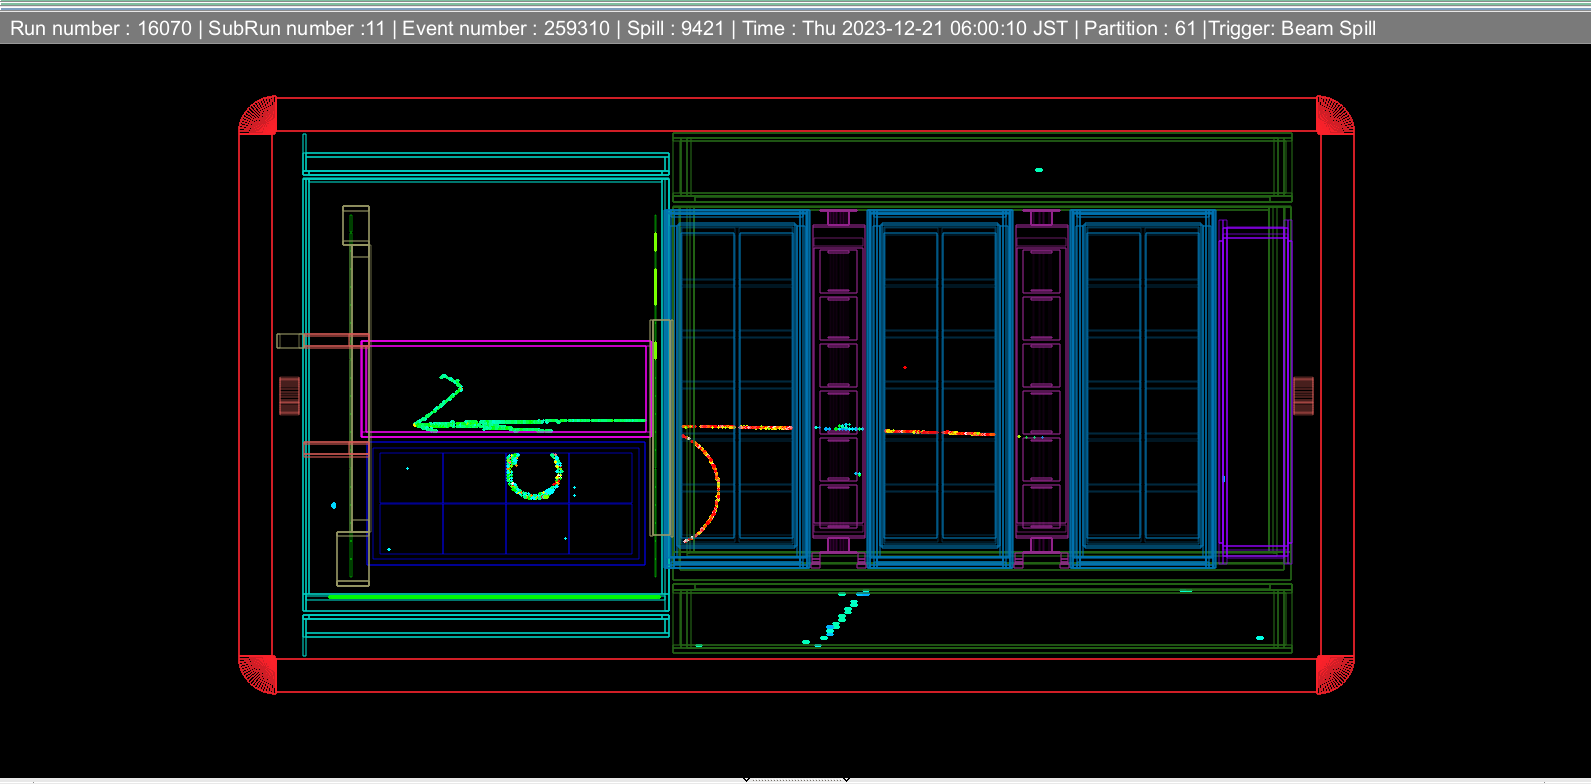
\includegraphics[width=0.5\linewidth]{fig/upgradeEvtDis.png}
        \caption{Event display of a possible $\pi^+$ event.}
        \label{fig:ndup-evedis}
    \end{figure}
\begin{savequote}[8cm]
Alles Gescheite ist schon gedacht worden.\\
Man muss nur versuchen, es noch einmal zu denken.

All intelligent thoughts have already been thought;\\
what is necessary is only to try to think them again.
  \qauthor{--- Johann Wolfgang von Goethe \cite{von_goethe_wilhelm_1829}}

Dancing is more important. --- Pauli
\end{savequote}

\chapter{\label{ch:2-neutrinos}The Field of Neutrinos}

\minitoc

\section{The Past}
\section{The Present}
\section{The Plans}


This document introduction won't serve as a complete primer on \LaTeX.  There are plenty of those online, and googling your questions will often get you answers, especially from \url{http://tex.stackexchange.com}.

Instead, let's talk a little about a few of the features and packages lumped into this template situation.  The \verb|savequote| environment at the beginning of chapters can add some wittiness to your thesis.  If you don't like the quotes, just remove that block.

For when it comes time to do corrections, there are two useful commands here.  First, the \verb|mccorrect| command allows you to highlight a short correction \mccorrect{like this one}.  When the thesis is typeset normally, the correction will just appear as part of the text.  However, when you declare \verb|\correctionstrue| in the main \verb|Oxford_Thesis.tex| file, that correction will be highlighted in blue.  That might be useful for submitting a post-viva, corrected copy to your examiners so they can quickly verify you've completed the task.

\begin{mccorrection}
For larger chunks, like this paragraph or indeed entire figures, you can use the \verb|mccorrection| environment.  This environment highlights paragraph-sized and larger blocks with the same blue colour.
\end{mccorrection}

Read through the \verb|Oxford_Thesis.tex| file to see the various options for one- and two-sided printing, including or excluding the separate abstract page, and turning corrections and draft footer on or off, and the separate option to centre your text on the page (for PDF submission) or offset it (for binding).  There is also a separate option for master's degree submissions, which changes identifying information to candidate number and includes a word count.  (Unfortunately, \LaTeX has a hard time doing word counts automatically, so you'll have to enter the count manually if you require this.)

\section{Cardiac Imaging}\label{app:imaging}

Within months of Röntgen's discovery of the X-ray in \mccorrect{1895}\cite{gagliardi_rontgen_1996}, cardiac pathology was being investigated via non-invasive imaging \cite{gagliardi_cardiac_1996}.  Over the intervening years, cardiac imaging modalities and techniques have advanced significantly.  Clinically, cardiac imaging is used for two broad purposes: diagnosis of pathophysiology and guidance of interventional procedures.  These applications impose different requirements on imaging equipment, image acquisition time, computational complexity, spatial and temporal resolution, and tissue discrimination.  The common diagnostic and interventional cardiac imaging techniques in current clinical practice are reviewed below.  An accessible introduction to the physics of medical imaging can be found in Webb's \textit{Introduction to Biomedical Imaging} \cite{webb_introduction_2002}.  A comprehensive overview of the use of imaging in clinical cardiology is presented in Leeson's \textit{Cardiovascular Imaging} \cite{leeson_cardiovascular_2011}.

\subsection{Diagnostic Imaging}
\label{sub:diagnostic}

Beyond the chest X-ray (`plain film'), the key non-invasive imaging modalities in diagnostic cardiology are echocardiography, magnetic resonance imaging, and X-ray computed tomography, which are reviewed below.  Nuclear medicine, including positron emission tomography (PET) and single-photon emission computed tomography (SPECT), are not discussed here, as they do not play a role in the chapters to follow.

\subsubsection{Echocardiography}

\begin{figure}
\centering\includegraphics[width=0.7\textwidth]{figures/sample/Gray498.png} 
\caption[Four-chamber illustration of the human heart.]{Four-chamber illustration of the human heart.  Clockwise from upper-left: right atrium, left atrium, left ventricle, right ventricle.}
\label{fig:fourchamber}\end{figure}

The use of acoustic waves for medical diagnosis, inspired by naval sonar, was initially developed in the 1940s \cite{gagliardi_ultrasonography_1996}.  By 1954, the first clinically useful cardiac ultrasound -- examining motion of the mitral valve in stenosis -- was reported \cite{edler_ultrasonic_1957}.  These early scans were one-dimensional images (`A-mode'), sometimes repeated to generate a time axis (`M-mode').   The sector-scanning probe was developed in the 1970s \cite{bom_ultrasonic_1971,griffith_sector_1974}, leading to the `B-mode' that a modern cardiologist would recognise as an echocardiogram.

\begin{savequote}[8cm]
\begin{CJK*}{UTF8}{min}
おれは海賊王になる男だ!!!
\end{CJK*}

I'll be the one to measure $\dcp$.
  \qauthor{--- Monkey D. Luffy}
\end{savequote}

\chapter{\label{ch:t2k}The T2K Experiment} 

\minitoc
The T2K experiment is a long-baseline neutrino experiment with the aim of measuring CP violation in the lepton sector through neutrino oscillation measurements.  
This chapter begins by describing the experimental setup and then provides a concise overview of the software, thereby laying the groundwork for the subsequent analyses.

\section{Hardware}
As a long-baseline experiment, T2K encompasses a near detector (ND280) and a far detector (Super-Kamiokande, often referred to as Super-K).  
Both detectors must discriminate between \(\numu\) and \(\nue\) to measure neutrino oscillations.  
Naturally, detecting neutrinos directly is impossible.  
Instead, each detector must be able to identify the different particles produced when neutrinos interact with its active material.  
Most commonly, such neutrino–nucleus interactions generate the corresponding leptons (i.e., electrons or muons) and various hadrons, including protons, neutrons, and light mesons such as pions.

The far detector, SK, is a large water Cherenkov detector.  
It detects particles by collecting the Cherenkov light emitted when they travel faster than the speed of light in water.  
Hadrons resulting from neutrino interactions typically lack sufficient energy to emit Cherenkov radiation, whereas leptons often exceed this threshold.  
Consequently, SK primarily observes electrons and muons, whose Cherenkov radiation forms ring-like patterns transverse to their direction of flight.  
Because the electron is lighter than the muon, its path is more prone to scattering, causing the electron’s Cherenkov ring to appear more diffuse than the muon’s, as illustrated in Fig.~\ref{fig:sk-e-mu}.

\begin{figure}
    \centering
    \begin{subfigure}[b]{\dbfigwid\textwidth}
        \centering
        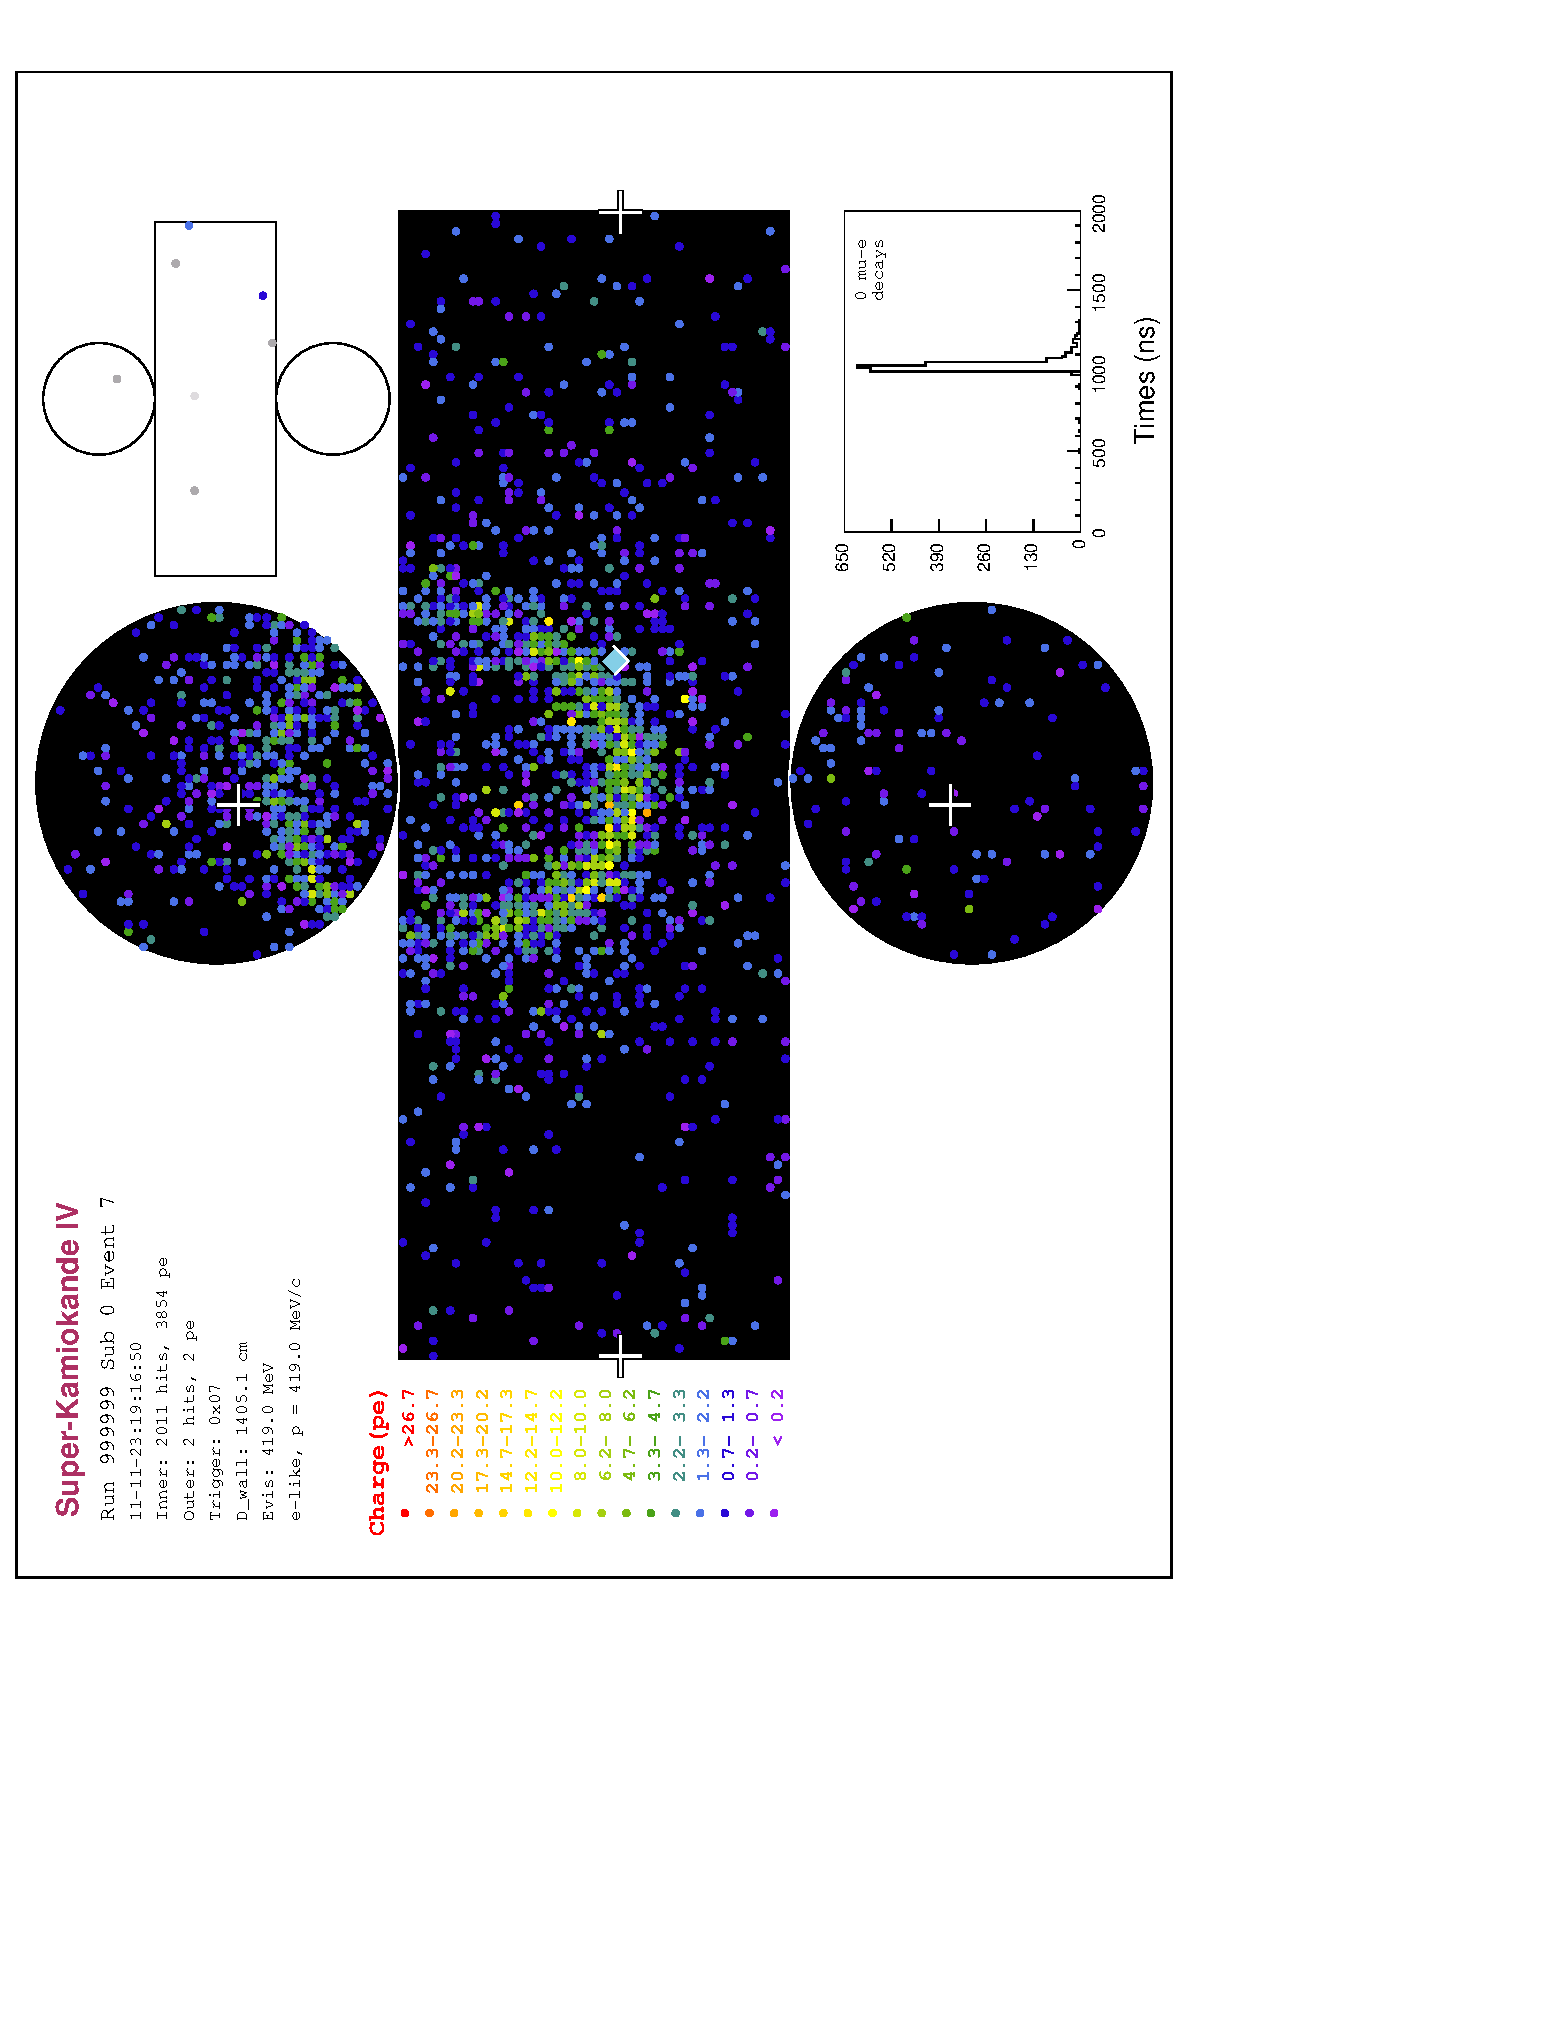
\includegraphics[width=\textwidth]{figures/t2k/sk-nue.eps}
        \caption{\(\nu_e\)}
        \label{subfig:sk-nue}
    \end{subfigure}
    \begin{subfigure}[b]{\dbfigwid\textwidth}
        \centering
        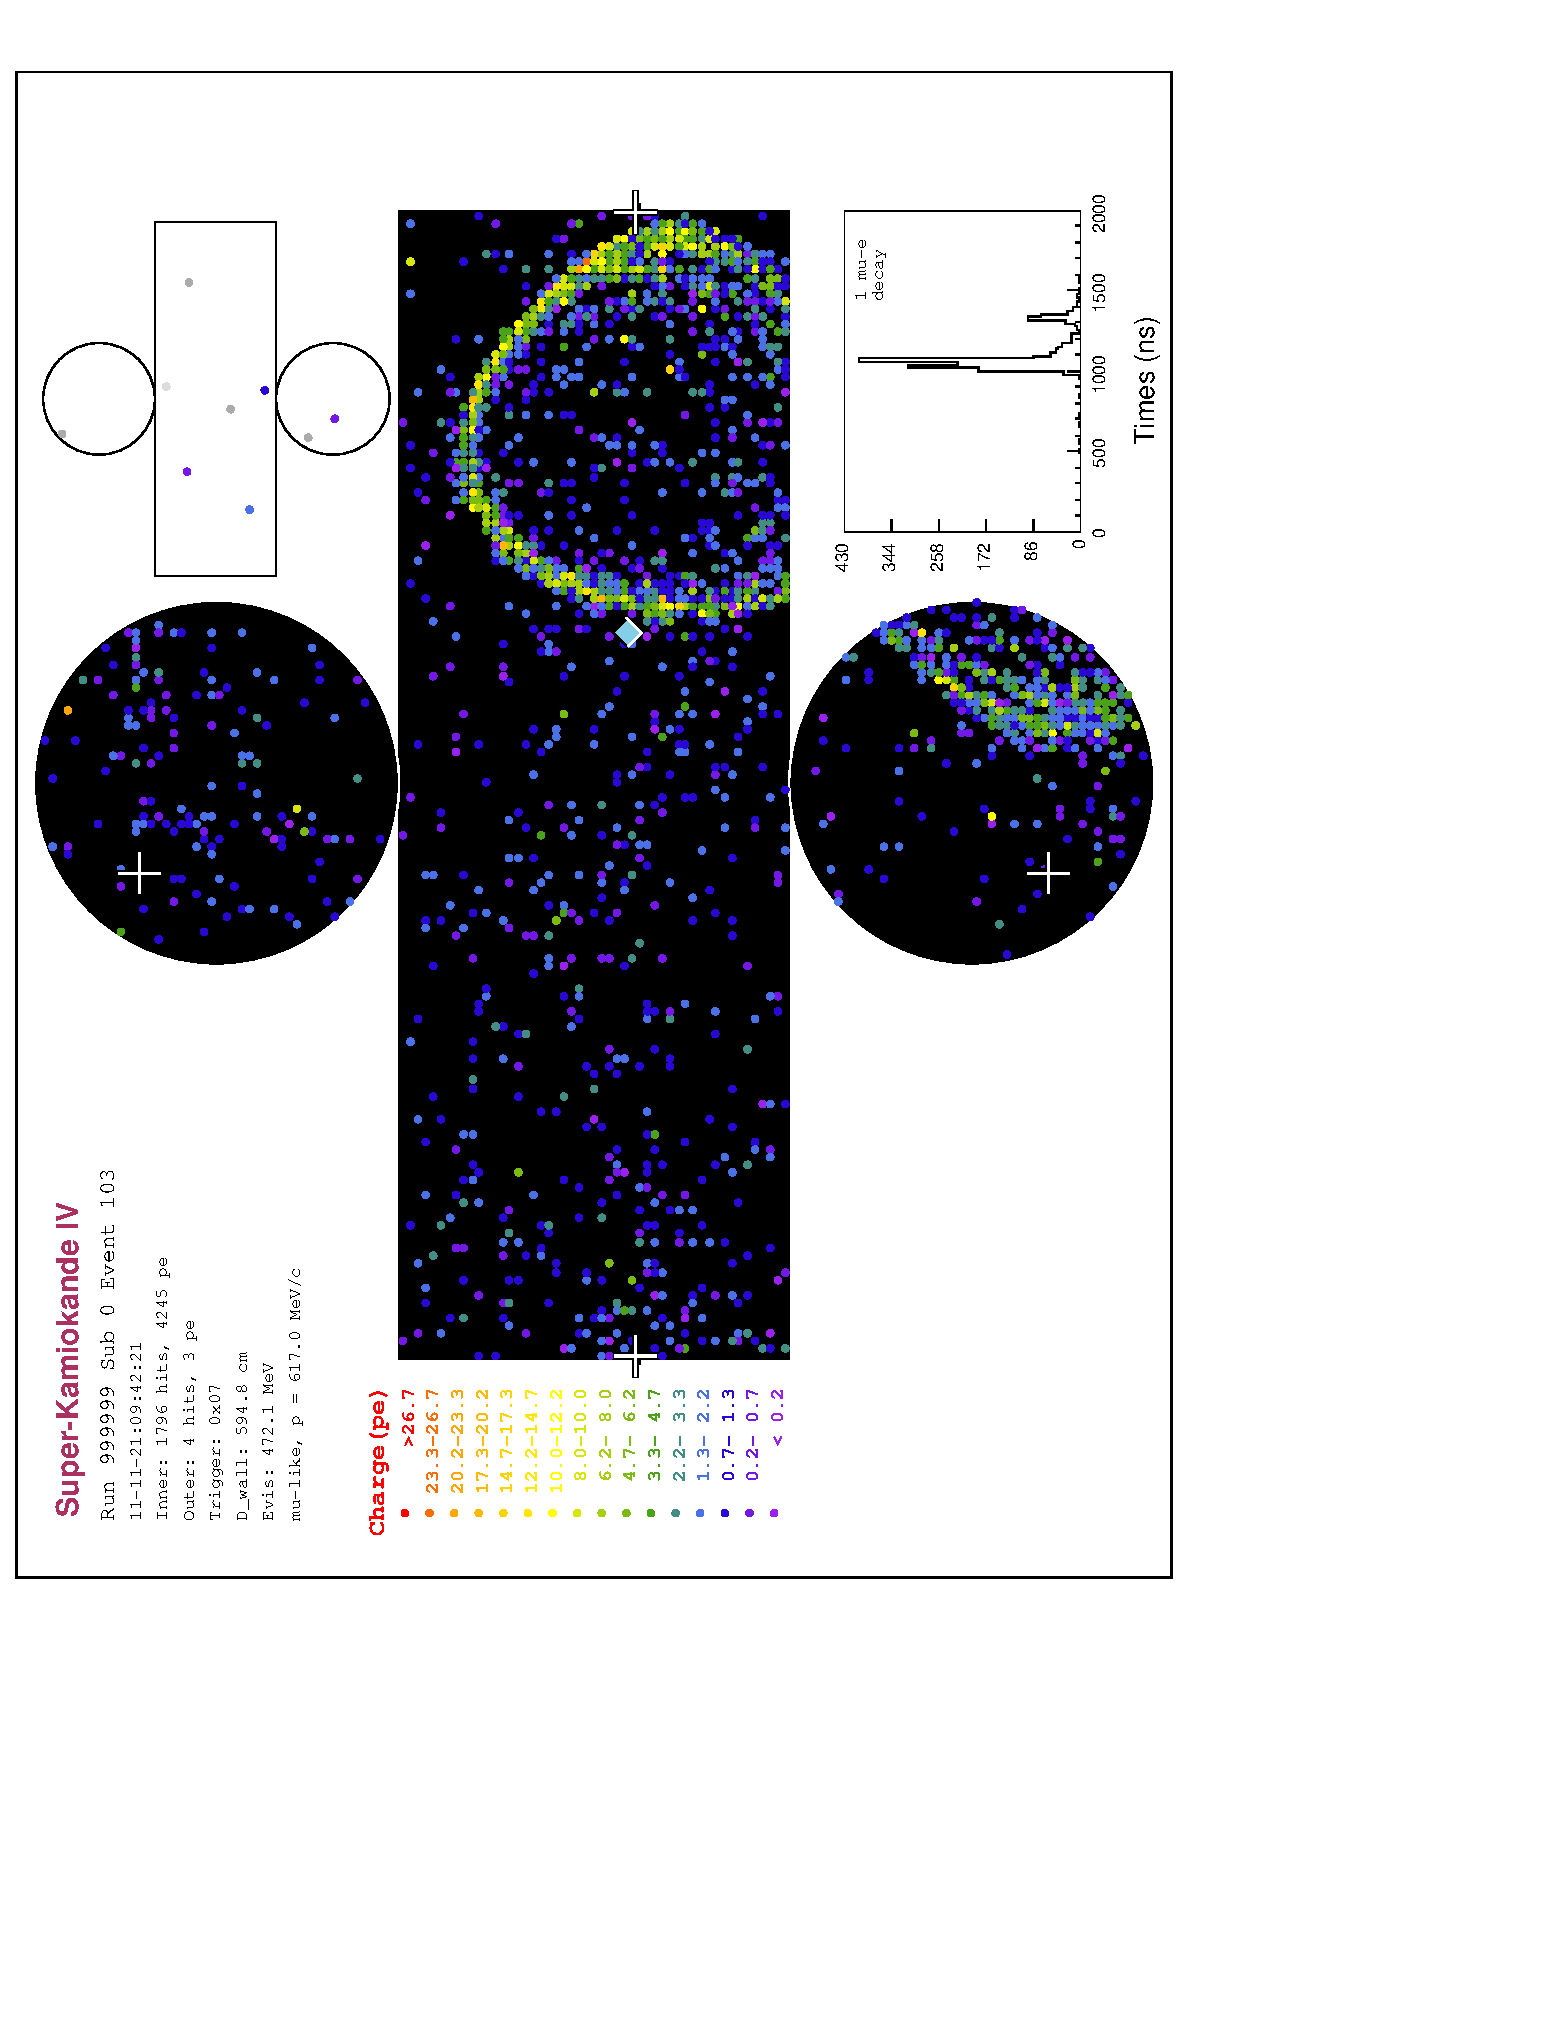
\includegraphics[width=\textwidth]{figures/t2k/sk-numu.eps}
        \caption{\(\nu_\mu\)}
        \label{subfig:sk-numu}
    \end{subfigure}
    \caption{SK event displays.}
    \label{fig:sk-e-mu}
\end{figure}

In contrast, the near detector, ND280, consists of multiple specialized subdetectors designed to measure hadrons.  
The classic ND280 configuration is shown in Fig.~\ref{subfig:nd280-classic}.  
Its central detector assembly contains a \(\piz\)-detector (P0D), three vertical Time Projection Chambers (TPCs), and two Fine Grained Detectors (FGDs) positioned between the TPCs.  
Surrounding these devices are various electromagnetic calorimeters (ECALs)—the P0D ECAL, the Barrel ECAL, the Upstream ECAL, and the Downstream ECAL—all enclosed by the UA1 magnet comprising a solenoid coil and a yoke.

\begin{figure}
    \centering
    \begin{subfigure}[b]{\dbfigwid\textwidth}
        \centering
        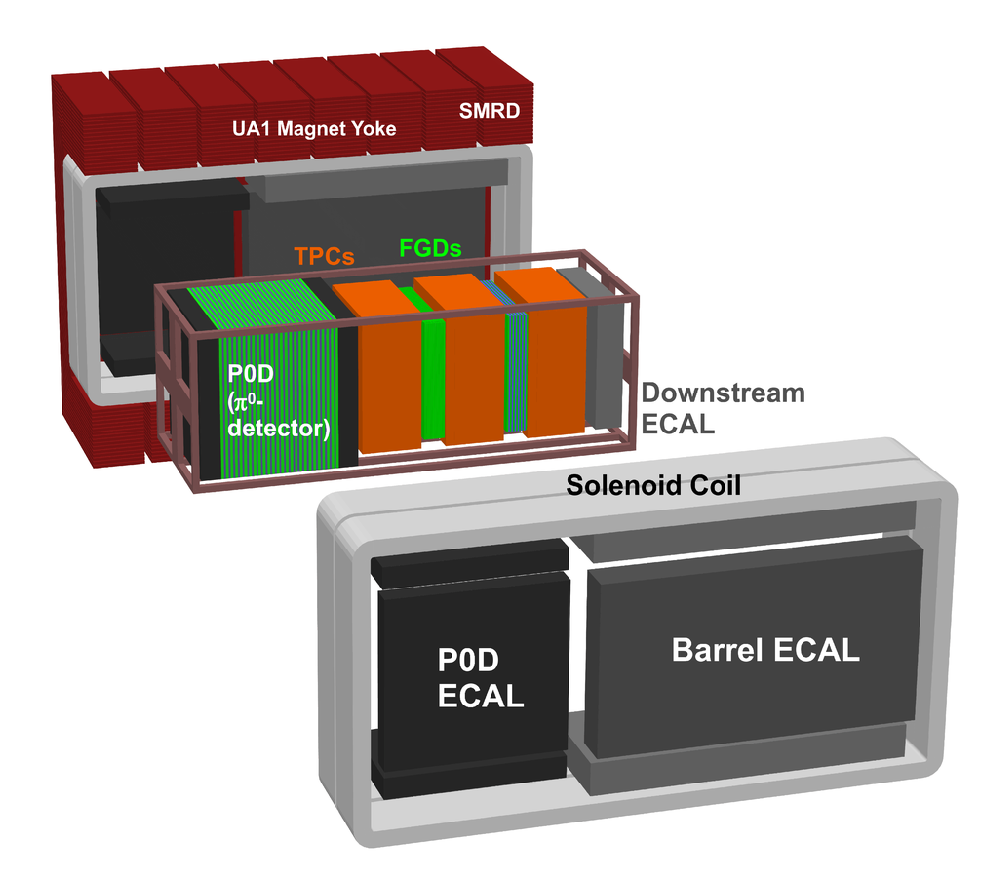
\includegraphics[width=\textwidth]{figures/t2k/ND280-classic.eps}
        \caption{Classic}
        \label{subfig:nd280-classic}
    \end{subfigure}
    \begin{subfigure}[b]{\dbfigwid\textwidth}
        \centering
        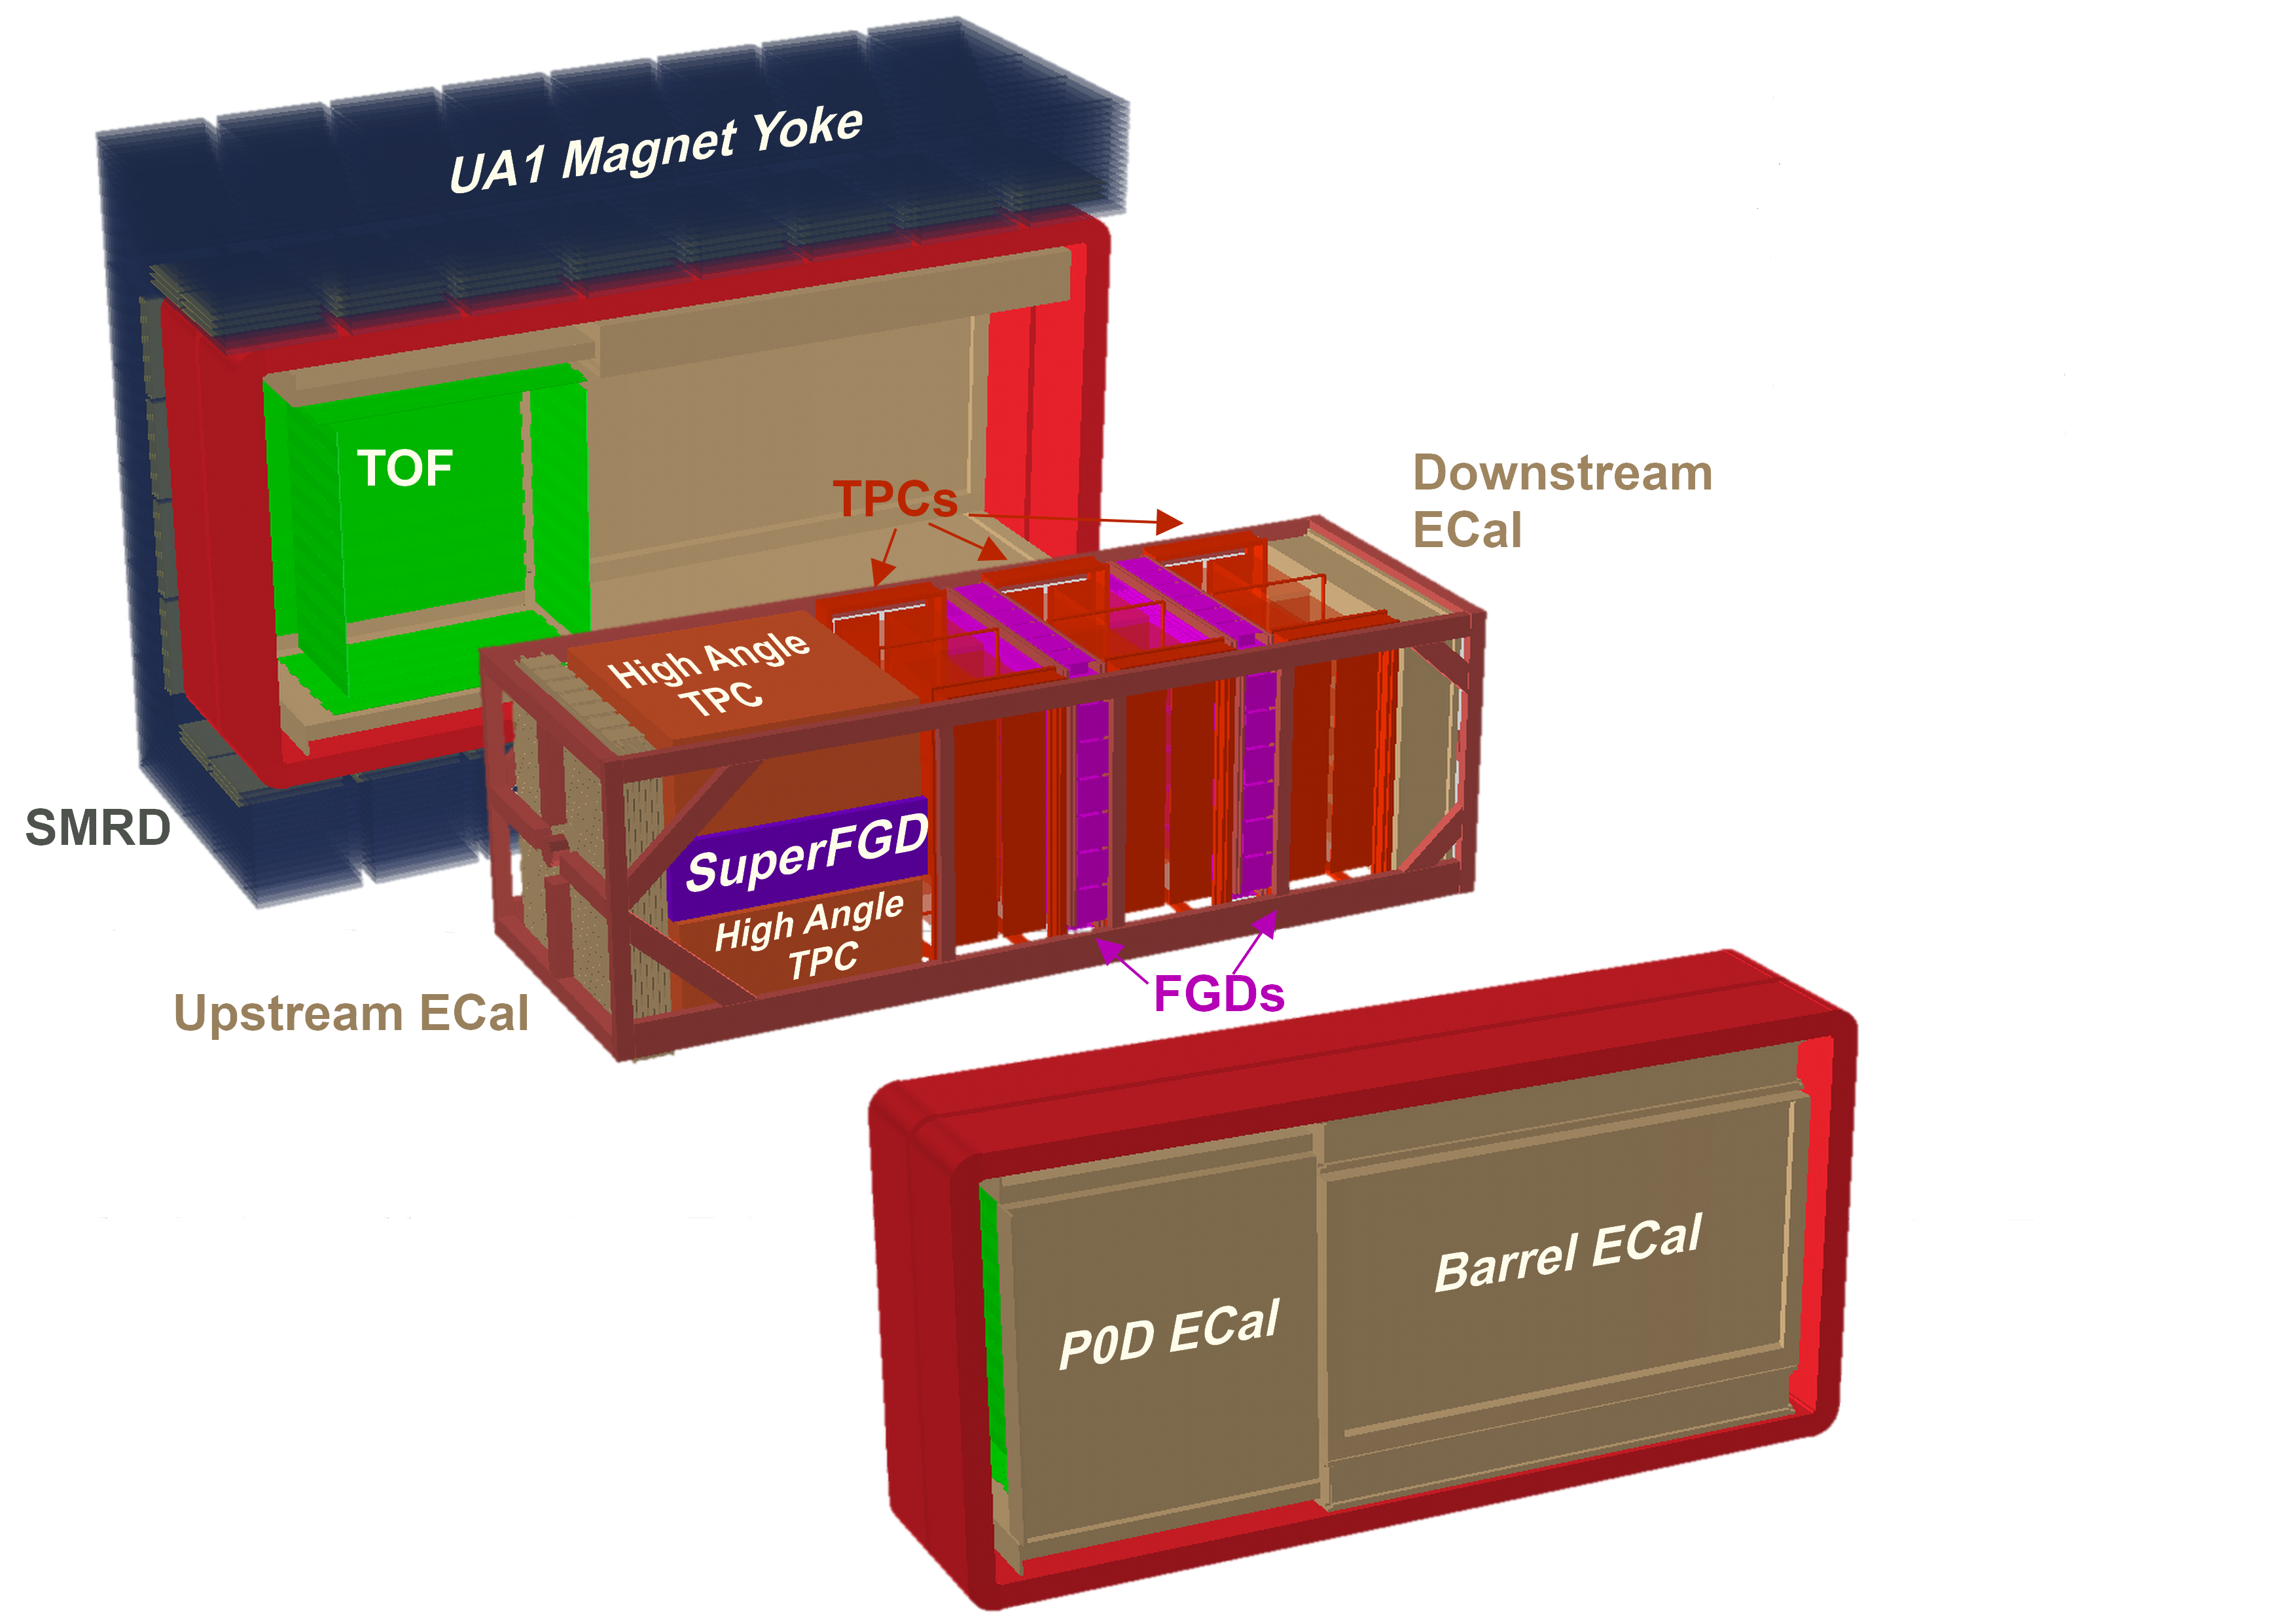
\includegraphics[width=\textwidth]{figures/t2k/ND280-up.png}
        \caption{Upgrade}
        \label{subfig:nd280-up}
    \end{subfigure}
    \caption{ND280 detector diagram.}
    \label{fig:nd280-diagram}
\end{figure}

The neutrino beam passes through the P0D, TPCs, and FGDs.  
Each FGD consists of scintillator bars with a cross section of \(1.0~\mathrm{cm} \times 1.0~\mathrm{cm}\).  
Every layer of bars is oriented orthogonally to the layer above it.  
As a particle traverses these layers, it excites photons in the scintillator; these photons are collected by wavelength-shifting fibers embedded in each bar and ultimately read out by end electronics.  
Hence, the bar recording the signal determines the track position transverse to the neutrino beam, while the layer index specifies the longitudinal position of the energy deposition.

Originally, FGDs served as the active target for neutrino interactions.  
However, their bar geometry offers limited acceptance for particles traveling at large angles to the beam direction—i.e., along the bar’s long axis—because such particles intersect only a few bars, making them difficult to reconstruct.  
This mismatch in phase space between the near and far detectors increases uncertainties in oscillation analyses.  
Moreover, having sparse signals along the particle trajectory degrades reconstruction resolution.  
These limitations motivated the ND280 upgrade.

In the upgraded ND280, the \(\piz\)-detector is replaced by several new subsystems (Fig.~\ref{subfig:nd280-up}): the Time-of-Flight detector (TOF), two High-Angle TPCs (HATs), and the Super Fine Grained Detector (SFGD).  
The TOF comprises six layers of scintillator bars with sub-nanosecond timing resolution, which help veto crossing particles and enhance sample purity.  
The HATs incorporate a redesigned field cage and new Micromegas detectors, expanding the tracking volume and improving resolution relative to the original vertical TPCs.  
Serving as the new active target, the SFGD consists of about two million \(1\,\mathrm{cm}^3\) scintillator cubes.  
Its finer segmentation markedly increases acceptance for high-angle tracks, better aligning with the near-isotropic acceptance at the far detector.  
Additionally, the improved tracking, enabled by enhanced energy deposition measurements, lowers detection thresholds and sharpens resolution, facilitating new reconstruction strategies (e.g., trackless pion reconstruction) and innovative variables (e.g., center-of-mass variables), which will be introduced in the next chapter.  
Construction for the upgrade was completed in April 2024, and data taking with the upgraded ND280 commenced in June 2024.

\section{Software}
\label{sec:t2k-sw}
This thesis focuses primarily on improving reconstruction performance; thus, the following overview of the software used for ND280’s upgraded system aims to clarify and contextualize the methodologies employed in later chapters.

Each scintillator cube in the SFGD contains an optical fiber, forming an electronic signal channel.  
As a charged particle traverses these cubes, scintillation photons are collected by readout boards located on three orthogonal faces of the SFGD.  
After calibration, these signals are digitized and assembled into three-dimensional “Hits,” each corresponding to a specific cube position and including a measure of deposited charge.  
The reconstruction software then sorts these Hits into either clusters or tracks using clustering and track-fitting algorithms.  
Clusters consist of fewer than three Hits, whereas tracks typically contain many more.  
Additionally, due to imperfect optical isolation between cubes, light may leak into neighboring cubes not actually traversed by the particle.  
To account for this, the reconstruction merges nearby Hits into “Nodes,” which more accurately capture the particle’s trajectory.  
Energy deposition at each Node is then estimated from the associated Hits and refined according to the expected continuous energy loss along the path.  
Finally, a Boosted Decision Tree (BDT), trained on Particle Gun simulations, uses these smoothed energy values and other measured parameters for particle identification and momentum estimation.  
\begin{savequote}[8cm]
\textlatin{Neque porro quisquam est qui dolorem ipsum quia dolor sit amet, consectetur, adipisci velit...}

There is no one who loves pain itself, who seeks after it and wants to have it, simply because it is pain...
  \qauthor{--- Cicero's \textit{de Finibus Bonorum et Malorum}}
\end{savequote}

\chapter{\label{ch:4-datamc}New Techniques and Data-MC Comparisons} 

The upgrade new detector has enhanced measuring capabilities. 
The granular structure of SFGD enables precise position and $\dedx$ measurements with fast response.
This is especially important for hadrons, as they tend to have much shorter tracks and are conventionally harder to reconstruct in scintillator detectors compared to muons.
As a result, the explored hadronic kinematic phase space is relatively restricted and the reconstructed hadronic variables have relatively large uncertainties.
Since more exclusive event topology such as $\numuccopiop$ allows the measurement of high-level variables like the Transverse Kinematic Imbalance (TKI) variables, which provide invaluable insights on neutrino-nucleus interactions, it is highly desirable to reconstruct hadrons, to measure their kinematic properties as precisely as possible and to explore their phase space as large as possible.
The T2K ND upgrade make possible the implementation of sophisticated techniques from other experiments, like the Elastically Scattered and Contained proton technique~\cite{Lu:2016mjf} that has shown significant improvement in proton momentum reconstruction resolution, and novel techniques implemented for the first time, i.e. the pion trackless reconstruction technique.
The benefits of these techniques will be illustrated based on MC studies and further showcase in data-MC comparisons for both low level variables, such as the single particle kinematic variables and the high level variables, like the Transverse Kinematic Imbalance (TKI) variables and the Centre-of-Momentum (COM) variables. 

\section{New Techniques}
\minitoc
   Two of the most common product hadrons from neutrino-nucleus interaction are protons and pions. 
   The default particle identification and momentum reconstruction have been developed by colleagues at T2K using the Boosted Decision Tree (BDT) algorithm. The BDT algorithm has good performance, but it is still lacking in some aspects.
   For instance, as it uses only single-track information, it cannot effectively distinguish between pions and muons. 
   It could reconstruct proton momentum with an excellent resolution of about $3.5\%$, but it is insufficient for TKI analysis, which is highly sensitive to hadron kinematics. 
   To address these gaps, I have developed and implemented new techniques for both hadrons. 
   For pions, I have invented the pion trackless reconstruction, a novel technique to reconstruct pions without requiring the presence of a reconstructed track, thereby lowering the detection threshold and significantly increasing reconstruction efficiency for low-momentum pions. 
   As for protons, I have adapted the Elastically Scattered and Contained (ESC) protons technique~\cite{Lu:2016mjf} first implemented in MINERvA to create an ESC proton selection in SFGD, leading to a proton sample with excellent momentum resolution. 

   %------------------- ESC ----------------%
  \subsection{ESC proton selection}

    \subsubsection{Working Principles}
    Protons stopping at rest would deposit a large amount of energy, the so-called Bragg Peak, just before it stops.
    These protons tend to have their momenta better constructed as its momentum is more strongly correlated with its range. 
    As shown in Fig.~\ref{fig:andedx2}, protons having energy below $1000$ units has large variances in momentum reconstruction. 
    \begin{figure}[h]
        \centering
        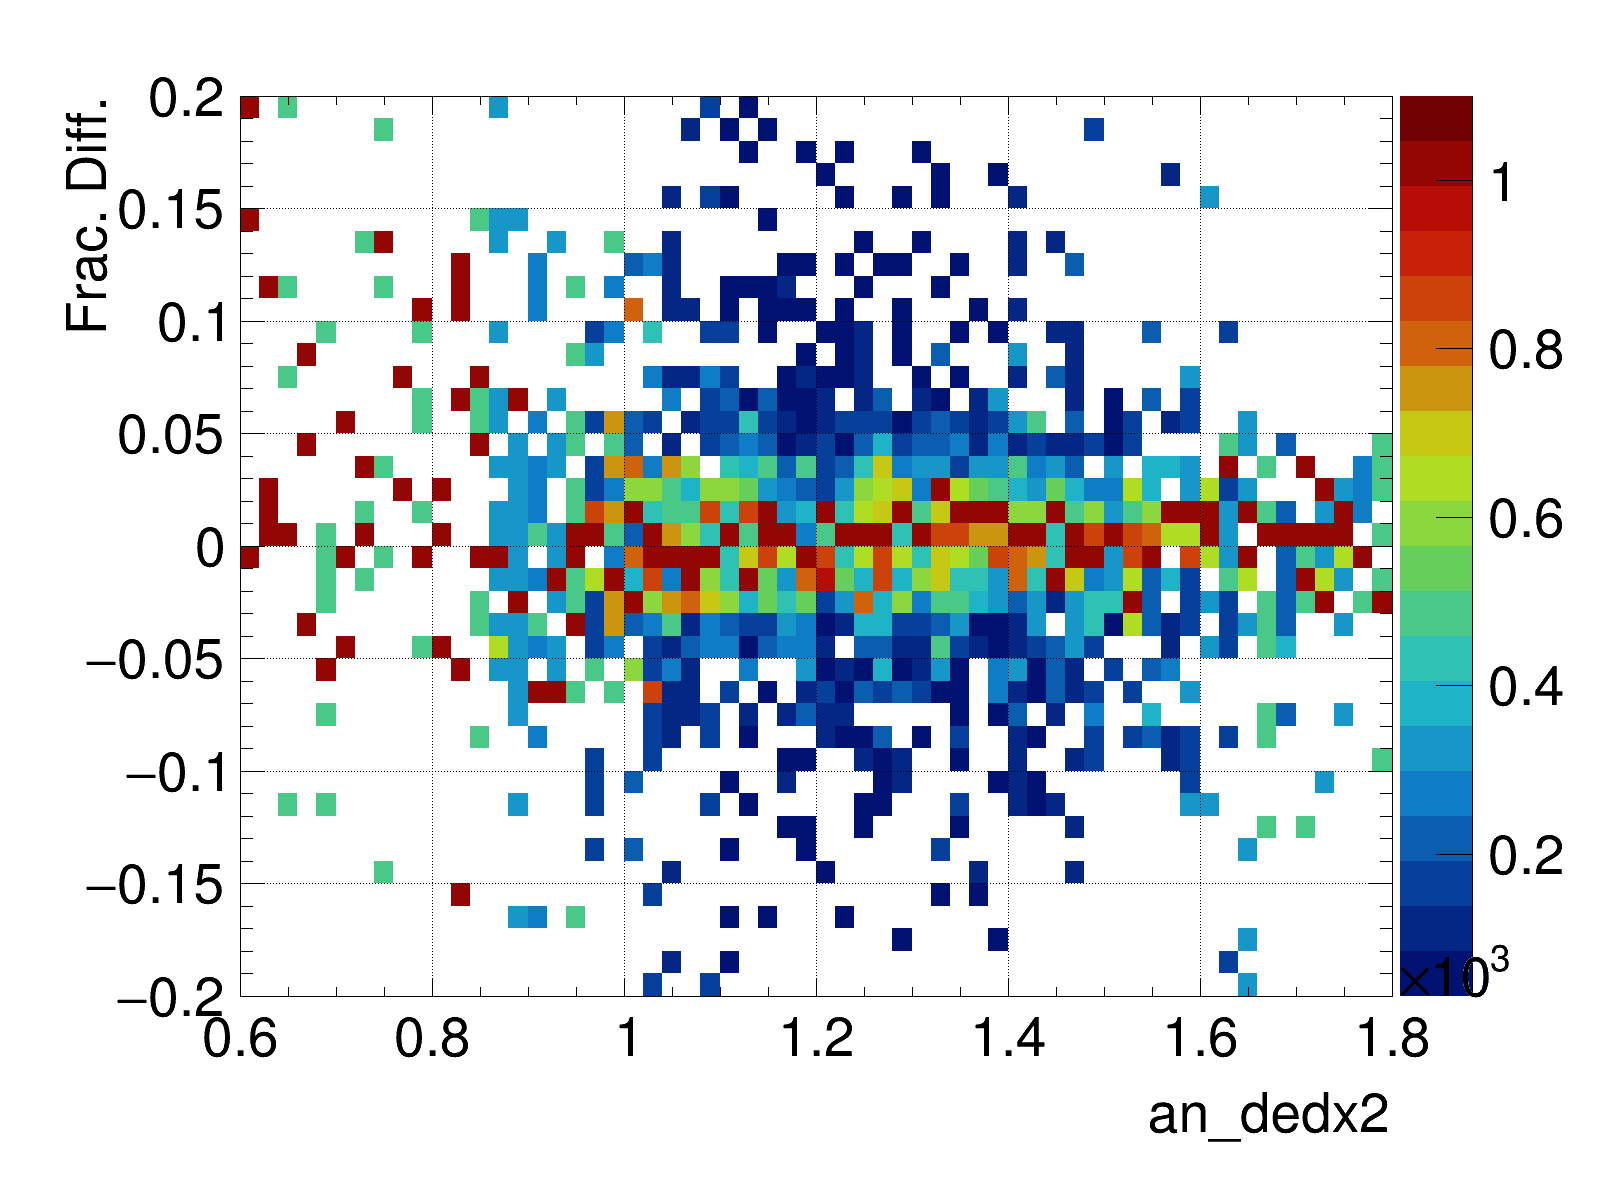
\includegraphics[width=0.5\linewidth]{fig/an_dedx2_colnor_vs_p_pr_res_hist2d_al12_zoom.png}
        \caption{Proton momentum fractional difference against energy deposited at the third last node.}
        \label{fig:andedx2}
    \end{figure}
    Hence, these protons can be selected by placing a lower boundary cut on the energy deposited at the nodes near the end of the reconstructed tracks to have a sample with a high proton momentum resolution.   
    
   \subsubsection{Implementation}
   As the ESC selection is based on $\dedx$ at the end of the proton track, a good reconstuction of $\dedx$ must be obtained first.
   To investigate the proper way of estimatiing $\dedx$, I have simulated multiple particle gun (PGUN) samples with the proton travelling in different directions in the SFGD.
   More specifically, three samples are travelling along the $x$-, $y$- and $z$-axis and five other samples are travelling at $15\degree$, $30\degree$, $45\degree$, $60\degree$ and $75\degree$ to the $x$-axis in the $x$-$z$ plane.
   As the proton direction should not affect its energy deposition, distinct characteristics of $\dedx$ along the proton trajectory can be utilized to validate the quality of the reconstructed $\dedx$.
   Other than the Bragg peak, another distinct feature of $\dedx$ is the minimal ionizing particle (MIP) region, where the particle at high momentum traverses the scintillator despositing the minimal amount of energy. 
   Hence, the $\dedx$ remains at a relatively constant value for all such particles.
   When the $\dedx$ at the end of the proton tracks are plotted, besides the Bragg peak at large $\dedx$, corresponding to protons stopping to rest, there should be another peak at smaller $\dedx$, corresponding protons that undergo secondary interactions and thus are stopped prematurely when it still possesses high momentum.

   The first attempt is to use the smoothed energy directly. 
   Fig.~\ref{fig:dedx-pgun-smoothed} plots energy deposit for the last third to sixth nodes for all PGUN samples travelling at different angles.
   It is reassuring to indeed observe the two peaks, the MIP peak and the Bragg peak, as hypothesized. 
   FIG-PGUN-DEDX-SMOOTH-bfANGNORM
   However, there are still some discrepancies. 
   The MIP peaks are close to each other, but their positions differ noticeably from each other.
   This is due to the different grouping of Hits into Nodes for protons travelling in different directions.
   The different number of Hits in a Nodes lead to different distances between nodes, so using the energy deposited per Node as an estimation of $\dedx$ is not strictly valid anymore.
   To account for the different propagation directions, I divided the energy by the sine of the angle of the trajectory made with the $z$-axis.
   The angle-normalized energy is plotted in Fig.~\ref{fig:dedx-pgun-angnorm}, which demonstrates that the angle-normalization step has achieved its goal - all MIP peaks have the same position.

   FIG-PGUN-DEDX-SMOOTH-afANGNORM

   Hence, the angle-normalized energy can serve as a good reconstruction of $\dedx$ for the ESC selection.
   To determine the suitable threshold $\dedx$ values without biasing the analysis with any underlying information in the signal sample, a stopping proton control sample is used.
   The stopping proton control sample has been developed by a colleague, which aims to select protons traversing one of the two HATs and stopping in SFGD. 
   For these stopping protons, their momenta can be reconstucted independently from HAT and SFGD.
   As momentum reconstruction in HAT (TPC) has high resolution and is well understood, the fractional difference between the reconstructed momenta in HAT and in SFGD for the same track is plotted against the angle-normalized energy to extract the range of $\dedx$ values that possess good momentum reconstruction in SFGD.
   For example, as shown in Fig.~\ref{fig:angnorm-dedx0}, a cut at xxxx should be placed.
   FIG-ANGNORM-dedx0
   FIG-ANGNORM-dedx1
   FIG-ANGNORM-dedx2
   FIG-ANGNORM-dedx3
   FIG-ANGNORM-dedx4
   FIG-ANGNORM-dedx5
   Hence, the respective thresholds for the last 6 nodes are xxx,xxx,xxx,xxx,xxx, and xxx, respectively.

   Furthermore, based on distributions of angle-normalized energy for the last 6 nodes, the average Bragg peak profile can be obtained by fitting the peaks of the distributions.
    The angle-normalized energy for the last 6 nodes for each track can then be compared with this average profile by a $\chi^2$,
    \begin{equation}
     \chi^2 = \Sum^6_1 \frac{(\dedx_i - \overline{\dedx_i})^2}{\overline{\dedx_i}}
    \end{equation}
    A proton coming to rest should have a similar profile, so an upper cut on $\chi^2$ could further select protons with good momentum resolution. 
    Similar to the determination of the threshold for the individual $\dedx$, the momenta fractional difference is plotted against $\chi^2$ as shown in Fig.~\ref{fig:esc-mom-res-chi2}.
    FIG-ESC-MOM-RES-CHI2
    The upper cut on $\chi^2$ is implemented as xxx.

    %------------------- pion TL ----------------%
    \subsection{Pion Trackless Reconstruction}
       As briefly elaborated in Sec.~\ref{sec:t2k-sw}, in SFGD, particle identification and momentum reconstruction are only performed on reconstructed tracks, which has a minimum length of about $30.0$~mm. 
       Hence, low-momentum particles, which travel only a short distance, could not be reconstructed at all. 
       When these low-momentum pions are not reconstructed, these $\ccopi$ events would then be misidentified as $\cczpi$ events, both decreasing the signal for the $\ccopi$ samples and increasing the background for the $\cczpi$ sample. 
       Thus, it would be highly beneficial if we could reconstruct these pions, and the pion trackless reconstruction technique I develop can address this gap perfectly. 

       \subsubsection{Working Principles}
         The trackless technique is an extension and sophistication of previous methods. 
         It was first tried in MINER$\nu$A\cite{MINERVAPOSTER} and in the Fine Grain Detectors of ND280\cite{T2KPOSTER}. 
         In the former, at least a reconstructed cluster is required to be identified as a pion candidate. 
         The latter indeed contains a prototype of the trackless reconstruction, but it is mixed with other pion reconstruction methods and its potential is not fully explored. 
    
         There are two key points of this reconstruction technique based on the pion decay chain, $\pi \rightarrow \mu \rightarrow e$.
         Firstly, the delayed signal of the grandchild, the Michel Electron (ME), is much longer than the time scale of other processes, such as $\piz$ decay.
         Hence, the presence of the primary pion can be inferred by the presence of a delayed signal in the SFGD.
         Secondly, the pion decay, $\pi \rightarrow \mu + \nu$, is a two-body process, the kinematics of the daughters can be completely determined by energy-momentum conservation, 
         When a pion decays at rest, the daughter muon will only move about $0.12~\textrm{cm}$. Hence, the starting point of the ME is a good estimation of the ending point of the pion.
         The pion momentum can then be reconstructed by range based on the distance between the primary neutrino interaction vertex and the ME starting point. 
         A relation between the pion momentum, via its kinetic energy, and its range is obtained from an empirical fit using a PGUN sample, as shown in shown in \figref{fig:fit}.
          The PGUN sample starts from the centre of SFGD and progates isotropically.
          It has a sample size of $500,000$ with a kinetic energy uniformly distributed between $20~\mev$ and $200~\mev$.
          The $\log10$ of the true kinetic energy is plotted against the true pion length as shown in Fig.~\ref{fig:pi-mombr-fit}.
          A fourth order polynomial is fitted to the central region of the plots, where the fitted line matches the data point well.

           \begin{figure}[h]
              \centering
              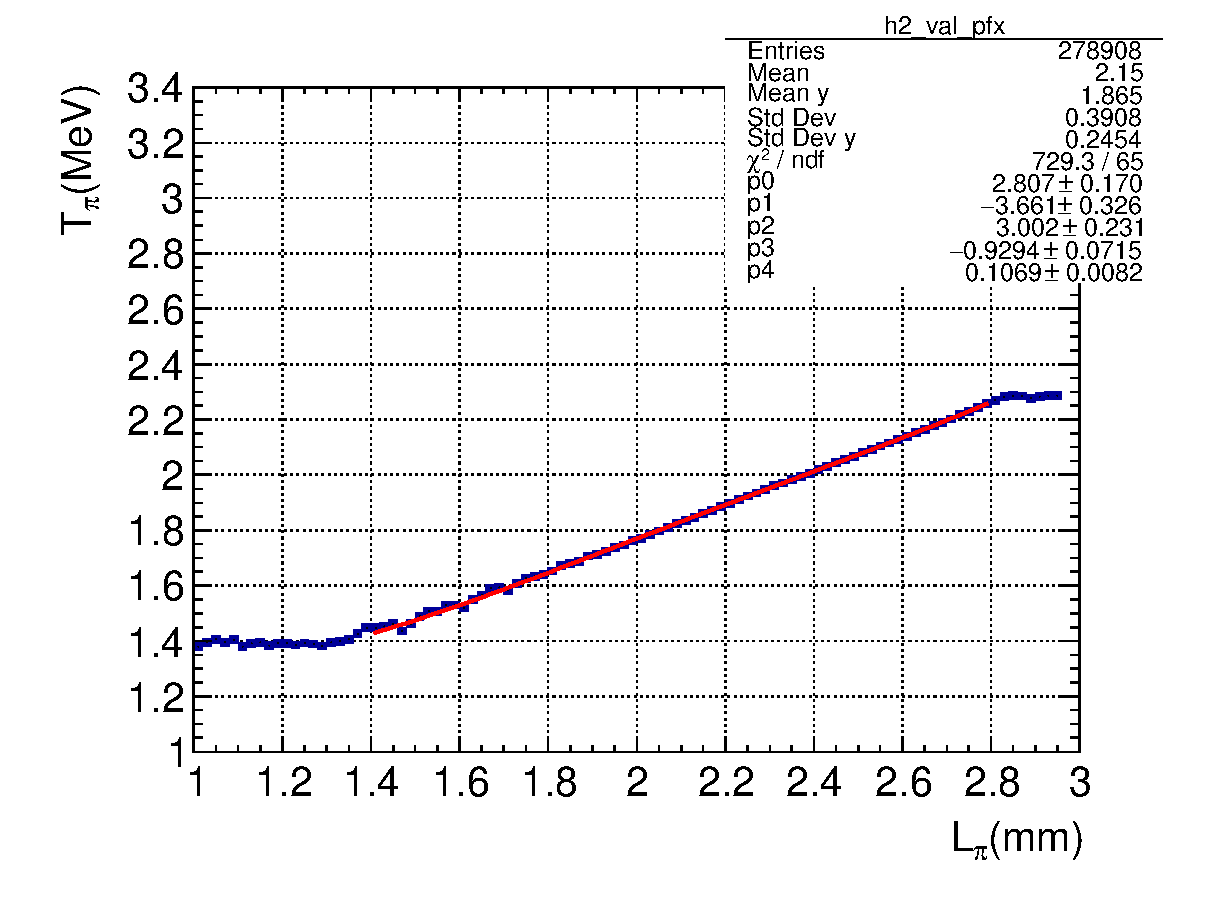
\includegraphics[width=\sgfidwid\textwidth]{figures/pi_len_pi_len_vs_pi_ke_hist2d_al0_true_nokink.eps} 
              \caption{A degree 4 polynomial fit of $\log_{10}{T_\pi}$ against $\log_{10}{L_\pi}$, where $T_\pi$ and $L_\pi$ are the kinetic energy and the range of the pion respectively. The $p_i$'s are the corresponding coefficients of the term of order $i$. The fit is satisfactory considering the close to 1 (\mccorrect{NOT TRUE}) $\chi^2/ndf$ value. }
              \label{fig:fit}
           \end{figure}

        \subsubsection{Implementation}
            The pion trackless reconstruction is part of my $\numuccopi$ selection, which is based on the existing $\numucc$-inclusive selection. Hence, it is best to elaborate the trackless technique in the context of the $\numuccopi$ selection. 
        
            The $\numucc$-inclusive selection has identified the primary vertex position and the primary muon, which already provides the trackless reconstruction with a good approximation of the pion starting point. The following steps are implemented to identify the suitable ME and reconstruct the pion momentum in the $\numuccopi$ selection. 

            \begin{itemize}
                \item Step 0 - \textbf{$\numucc$-inclusive selection.}
                \item Step 1 - \textbf{Find suitable ME candidates.} 
                \item Step 2 - \textbf{One trackless pion cut.}
                \item Step 3 - \textbf{Kink cut.}
                \item Step 4 - \textbf{Background reduction.}
            \end{itemize}
        
            \textbf{Find suitable ME candidates.} - Loop through all delayed reconstructed objects that have more than 1 hit, if it is $30.0~\textrm{ns}$ after the primary vertex time, save it as a potential ME candidate. 
            However, it is common that the ME could trigger a shower, leading to more delayed reconstructed objects. 
            To distinguish the ME from these secondary delayed objects, a technique called the "prompt energy" was used by MINERvA~\cite{Zhang2016}. 
            Prompt energy is the energy deposited by the short muon and the short pion. 
            Even though these particles might have too low energy to leave a reconstruct-able track, they would still deposit energy, which is much early than the onset of ME. 
            Hence, looping through the cubes $30.0~\textrm{mm}$ around the two ends of an ME candidate to observe if there is energy deposited $30.0~\textrm{ns}$ before identifying the proper ME candidate. 
            Moreover, if the primary muon is contained in SFGD, it would also decay to give an ME, which is indistinguishable from a pion ME by just looking at the time delay. 
            Hence, an additional check is added to exclude ME candidates near the end of the identified primary muon. 
        
            \textbf{One trackless pion cut} - Select events that have one and only one proper ME candidate.
        
            \textbf{Kink cut} - As the trackless reconstruction does not require the ME to be near a primary track, it cannot distinguish pions travelling straight from the primary interaction until decaying at rest from those that have undergone a deflection and then decayed at rest. 
            Events with a deflected pion should be rejected as the momentum-by-range reconstruction works only for particles without secondary interaction. 
            Hence, events with an ME connected to any non-primary tracks would be rejected.
        
            \textbf{Background reduction} - Several background reduction steps are implemented, for example, an existing $\pi^0$ rejection developed by Colleagues at T2K.
            However, they are insufficient as shown by the considerable portion of CC-other backgrounds in Fig.~\ref{fig:tlpi-bf-trknumcut}.
            FIG-TLPI-BF-trknumcut
            Hence, based on logical understanding of different event topologies, I developed a series of track number cuts and a new idea, called the track family tree.
            
            An event topology resembles a family tree sideway. 
            The first generation contains the primary tracks.
            The second generation are tracks connecting to the end of the primary tracks.
            The family tree tracing step loops through all reconstructed tracks to form the family tree starting from the primary vertex.
            One useful variable is the number of generations.
            A $\numuccopi$ event should not contain a large number of generations as the primary pion can have an ME attached to its end, but there is no shower or multiple scattering.
            Hence, the number of generation is required to be smaller than $3$.
            Another associated variable is the number of lone tracks, which are not connected to any tracks in the family tree. 
            A clean $\numuccopi$ event should have a limited number of lone tracks, which could be due to noise, or low energy scattering of the ME, which leads to clusters isolated from the ME track. 
            More details of the other track number cuts are provided in Appendix.~\ref{sec:app-tlpi-trknumcut}
        
            For the events passing all the selection steps, the presence of a primary pion is implied by the existence of a proper ME candidate, and its momentum is reconstructed by range. 


    \subsection{Development of stopping pion control sample}
          Conventionally, selections will be used for cross section analysis, which requires a sufficient portion of all detector systematics to be properly evaluated.
          However, due to time constraint, this is unlikely to happen within the time frame of my doctoral study. 
          Hence, only preliminary data-MC comparisons are possible.
          Nontheless, as systematics evaluation is an important ingredient of cross section analysis, which is crucial for improving our understanding of neutrino-nucleus interactions, I implemented the propagation of the systematics of the momentum-by-range reconstruction for pions tagged by ME.
          To evaluate this systematic, I developed the stopping pion control sample with the following steps:
          \begin{enumerate}
          \item Find all tracks that contain an SFGD segment and segments in the other sub-detectors.
          \item Check that one end of this track is stopped in SFGD.
          \item Check the PID of this track provided by the other sub-detectors, i.e. HAT or TPC.
          \item Check that there are no other (except ME) near the track end in SFGD.
          \item A final cut requiring the presence of an ME near the track end in SFGD.
          \item Keep only the event with a single stopping pion candidate.
          \end{enumerate}
          The preliminary result suggests that the control sample consists predorminantly of tracks passing HAT and stopping in SFGD.
          As the current PID in HAT is not fully developed, I investigated further the impact of the log likelihood on pion PID.
          I discovered that the previous cuts need to be made more stringent to achieve a high purity.

          FIG- HAT LLH cuts

           
    
    

\section{MC studies and Comparisons with Data}

   The lower boundary cut is implemented as an extra step on the existing $\numuccopiop$ sample, where the $p$ stands for proton.
   This selection leads to an improvement in proton momentum resolution of about $50\%$ while decreasing the efficiency by about $2/3$, as shown in Fig.~\ref{fig:pprESC-res}.   
   The drop of efficiency might seem drastic, but it proves to be necessary for the TKI analysis, as shown later in Sec.~\ref{sec:do-TKI}. The ESC selection leads to significant improvement to the TKI variables evaluation. 

   \begin{figure}[t]
      \centering
      \begin{subfigure}{0.45\textwidth}
           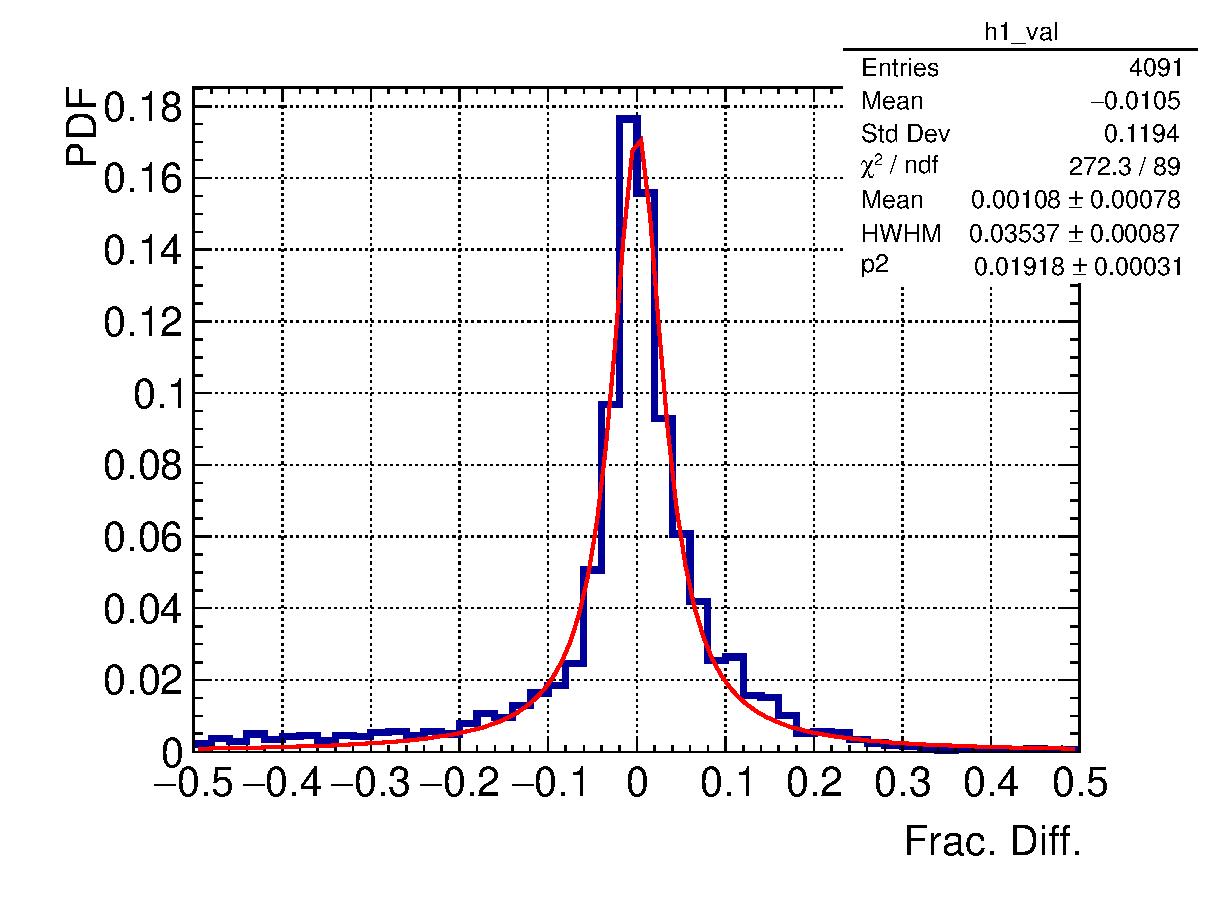
\includegraphics[width=\textwidth]{fig/p_pr_res_pdf_al13_zoom.eps}
           \caption{Momentum resolution before ESC selection.}
           \label{fig:ppr-res-bfESC}
      \end{subfigure}
      \begin{subfigure}{0.45\textwidth}
           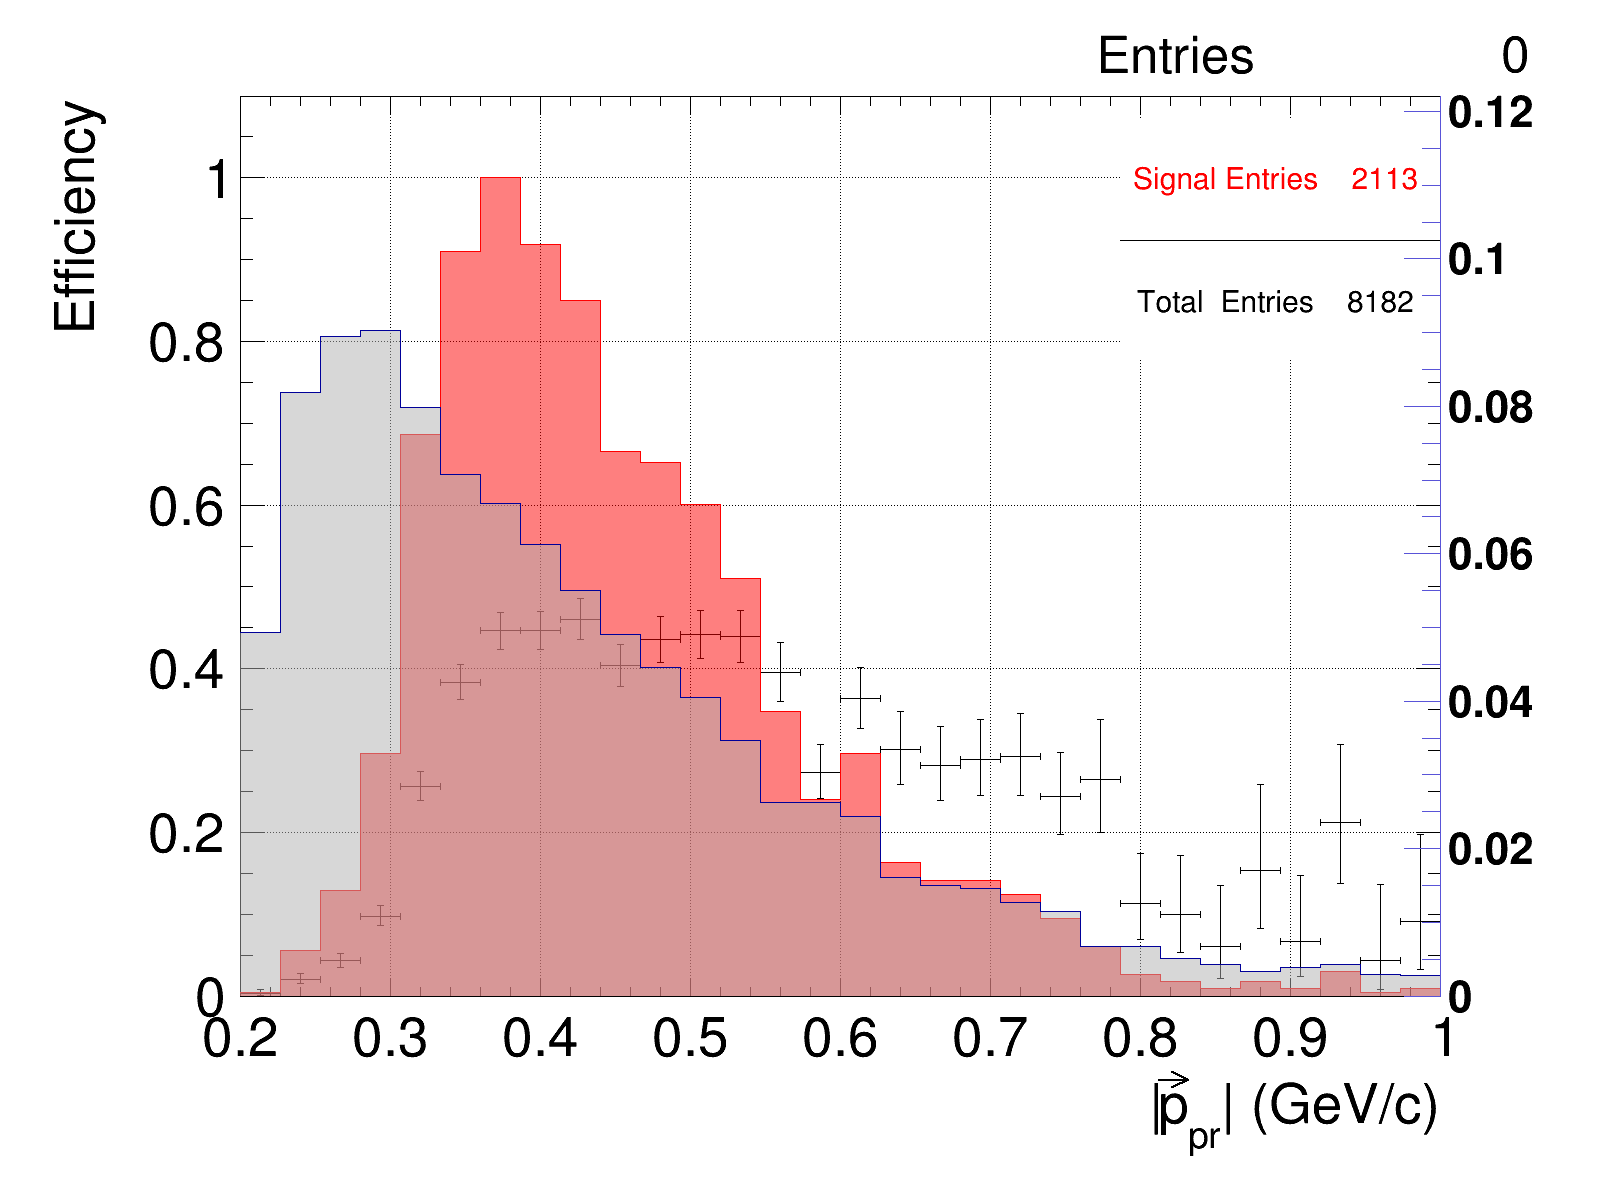
\includegraphics[width=\textwidth]{fig/p_pr_eff_al13.png}
           \caption{Selection efficiency before ESC selection.}
           \label{fig:ppr-eff-bfESC}
      \end{subfigure}
      \\
      \begin{subfigure}{0.45\textwidth}
           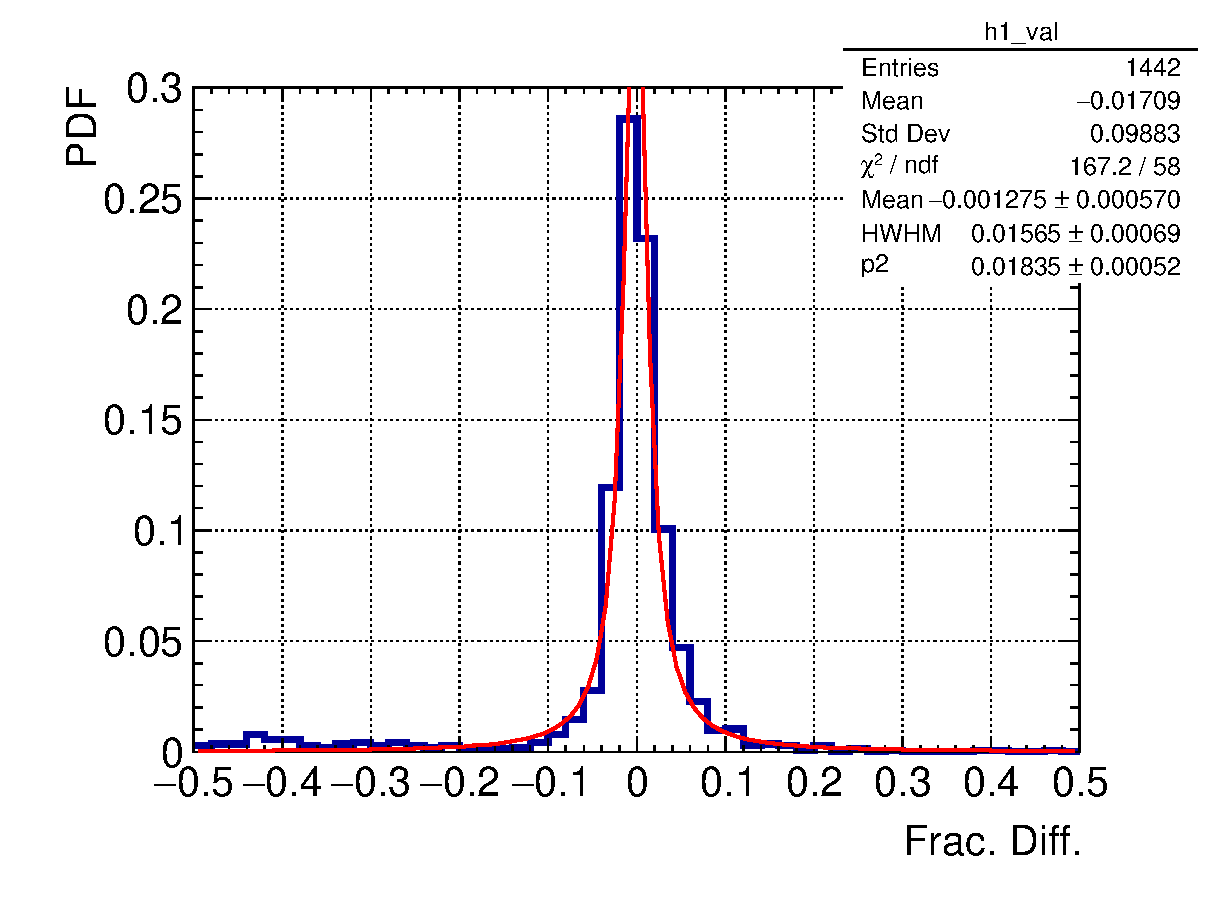
\includegraphics[width=\textwidth]{fig/p_pr_res_pdf_al14_zoom.eps}
           \caption{Momentum resolution after ESC selection.}
           \label{fig:ppr-res-afESC}
      \end{subfigure}
      \begin{subfigure}{0.45\textwidth}
           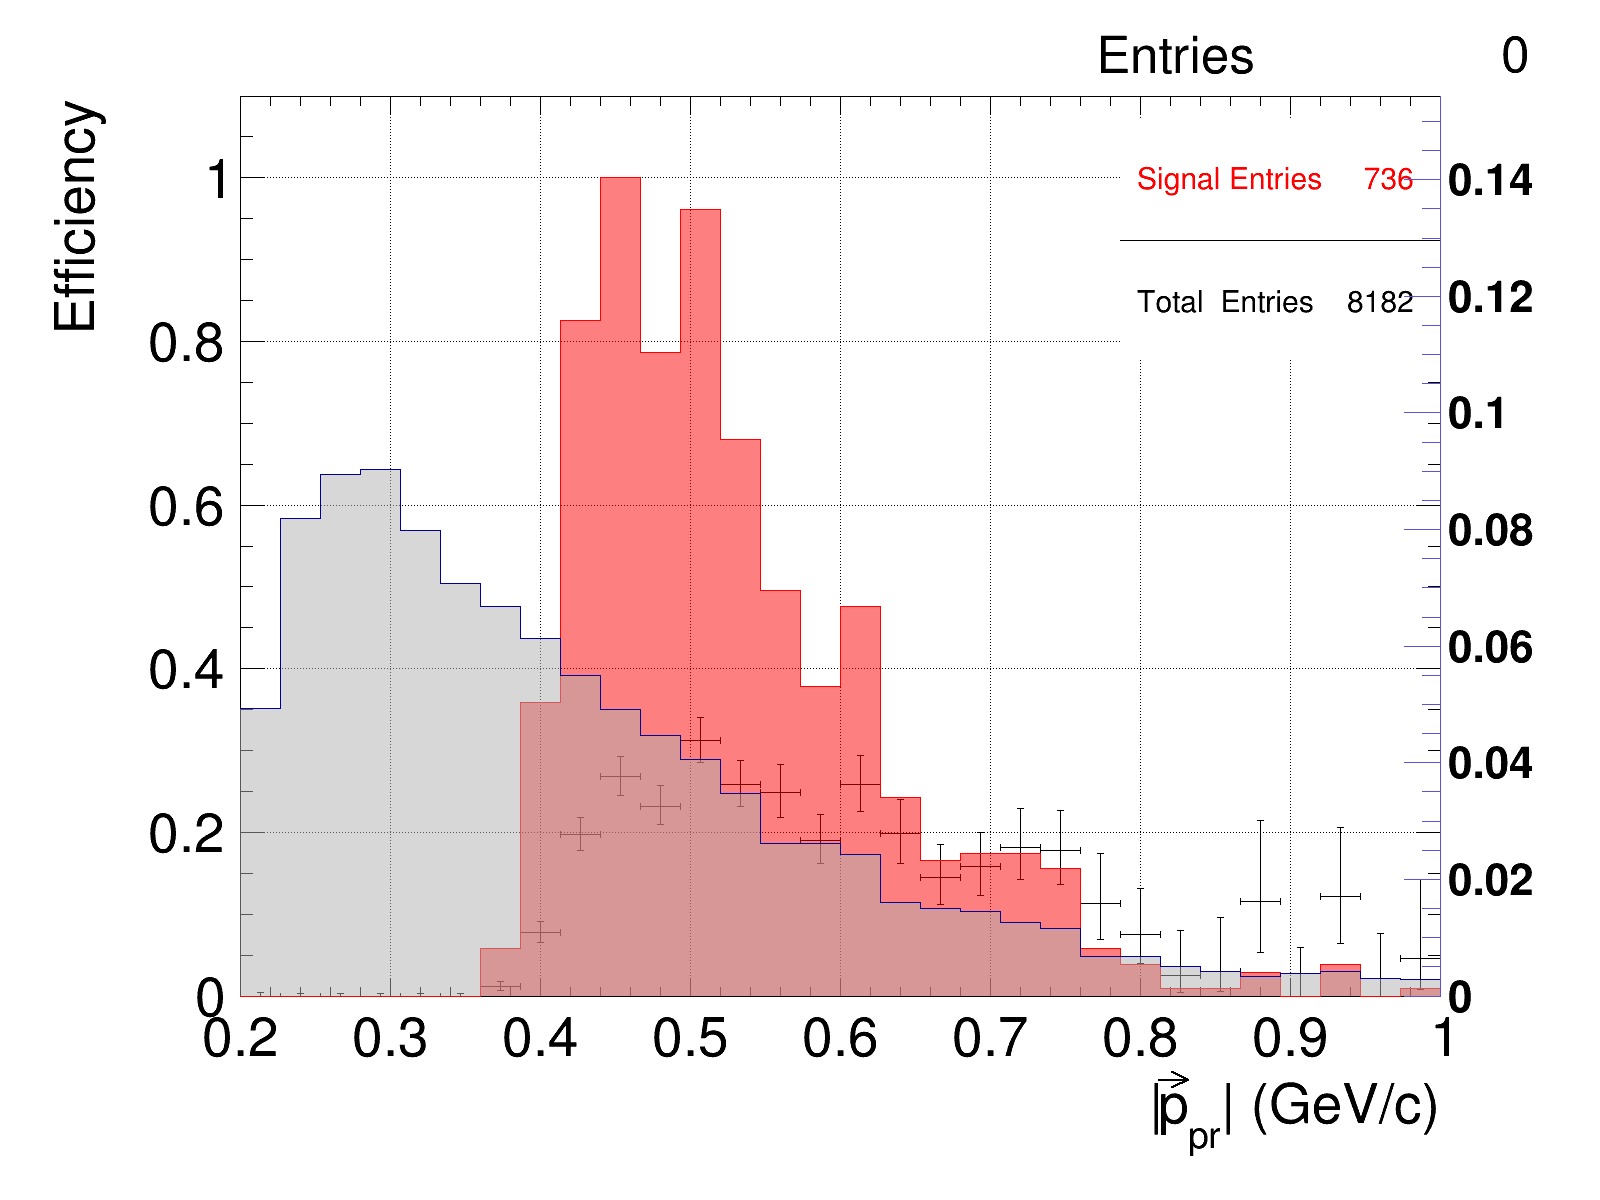
\includegraphics[width=\textwidth]{fig/p_pr_eff_al14.png}
           \caption{Selection efficiency after ESC selection.}
           \label{fig:ppr-eff-afESC}
      \end{subfigure}
      \caption{Proton ESC selection results. The grey histograms are the true probability distribution, while the pink ones are those that get reconstructed. }
      \label{fig:pprESC-res}
   \end{figure}

    
        \subsubsection{Results}
           The results of the $\numuccopi$ selection using the trackless pion technique are summarised in Fig.~\ref{fig:piTLres}.
           As shown in Fig,~\ref{fig:ppi-stack}, the trackless selection has achieved the set goal - reconstructing low momentum pions. 
           There are a considerable number of events with a pion below $100~\mevc$, which correspond to a track of about $50~\textrm{mm}$. 
           Moreover, pions below $80~\mevc$ have also been reconstructed, which travels about $30~\textrm{mm}$ and cannot be reconstructed as a track. 
           Furthermore, the momentum-by-range calculation has achieved an excellent resolution at about $2\%$, as shown in $\ref{fig:ppi-res}$.
           More encouragingly, the overall efficiencies are still relatively high. 
           The step-by-step efficiencies with respect to each step is shown in Fig.~\ref{fig:tl-accum-eff}. 
           The signal definition used in the calculation is to have one true muon that has travelled to the vertical TPC and one true pion that is contained in SFGD. 
           Steps 1 to 7 are the $\numucc$-inclusive selection. 
           The large drop in efficiency in Step 8 is expected as it requires exactly one pion reconstructed tracklessly. 
           All pions undergoing secondary interactions except deflection cannot be reconstructed via this method. 
           Hence, the relative efficiency of $0.37/0.66\approx56\%$ is considerably high. 
           The further significant drop in efficiency comes with the next step, the kink cut, which is a reasonable as a considerable portion of pions undergo deflection. 
           The subsequent drops are graduate cuts to remove backgrounds, which leads to a high purity of $\numuccopi$ as shown in Fig.~\ref{fig:ppi-stack}.

           \begin{figure}[t]
               \centering
               \begin{subfigure}{0.3\textwidth}
                    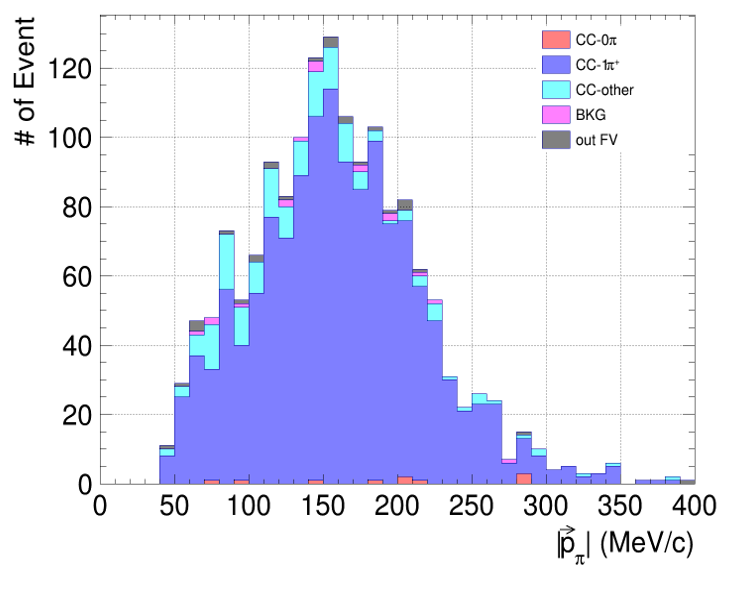
\includegraphics[width=\textwidth]{fig/ppi_stack.png}
                    \caption{Momentum distribution.}
                    \label{fig:ppi-stack}
               \end{subfigure}
               \begin{subfigure}{0.3\textwidth}
                    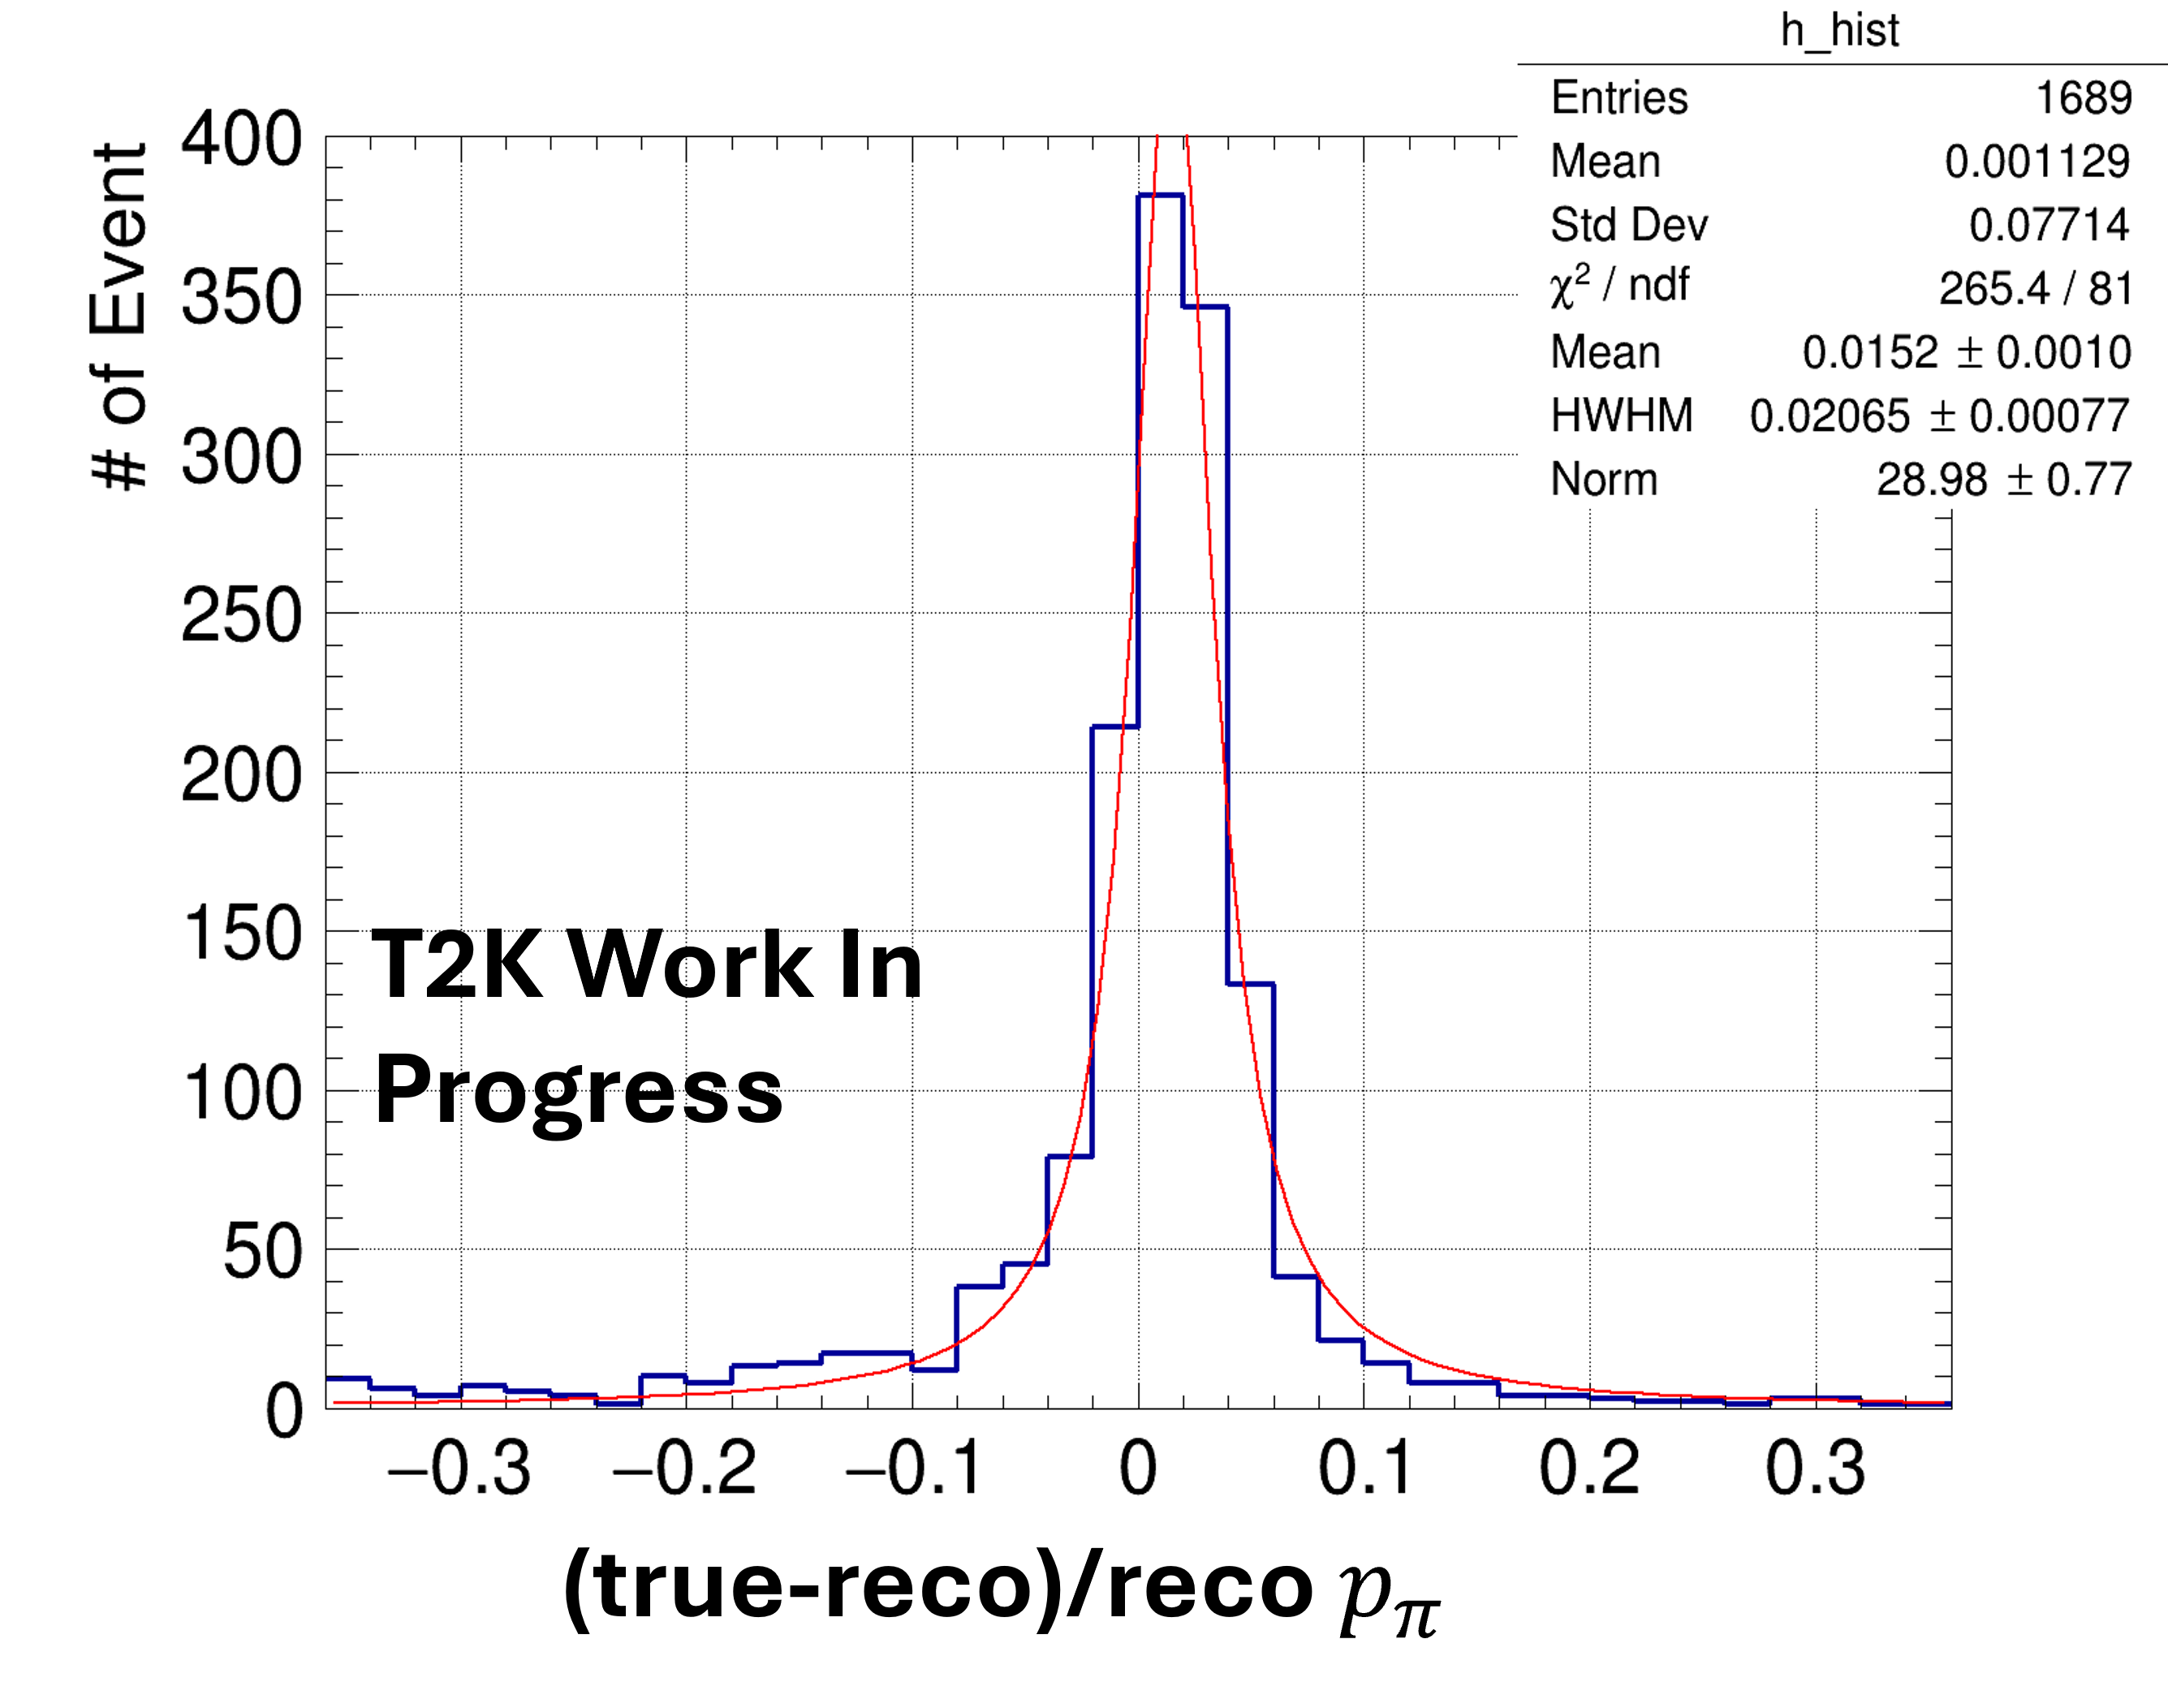
\includegraphics[width=\textwidth]{fig/ppi_res.png}
                    \caption{Momentum resolution.}
                    \label{fig:ppi-res}
               \end{subfigure}
               \begin{subfigure}{0.3\textwidth}
                    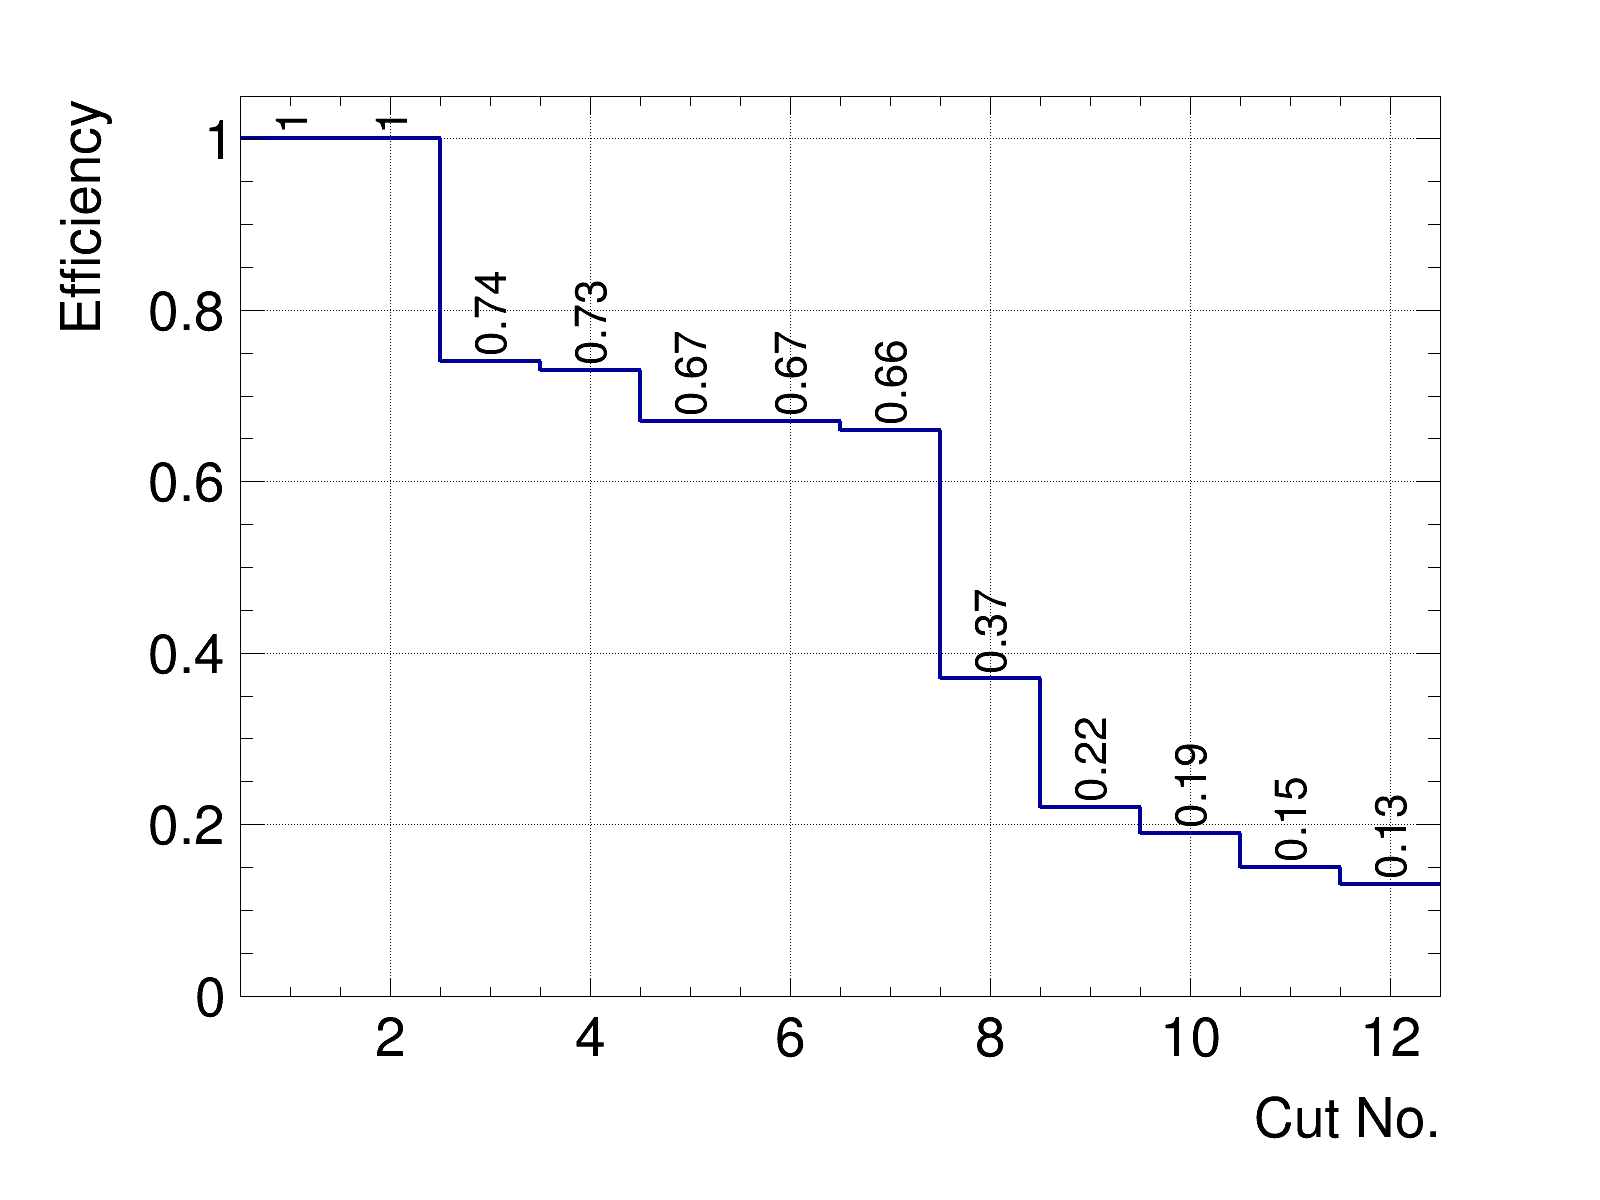
\includegraphics[width=\textwidth]{fig/INCL_p_pi_accum_eff_al11.png}
                    \caption{Accumulative efficiency.}
                    \label{fig:tl-accum-eff}
               \end{subfigure}
               \caption{Pion trackless reconstruction results.}
               \label{fig:piTLres}
            \end{figure}


            

    \subsection{Discussion}
        Both the pion and ESC proton selections are finished for muons going into the vertical TPC and SFGD. The High Angle TPC reconstruction is under development and will be expected to finish in the end of July 2024. Hence, the full selection will be done in the following months. The estimation of systematic uncertainties using control samples is being developed by colleagues and is expected to be done in the next few months. 


     \subsection{systematics ovaluation}
          
\begin{savequote}[8cm]
\textlatin{Neque porro quisquam est qui dolorem ipsum quia dolor sit amet, consectetur, adipisci velit...}

There is no one who loves pain itself, who seeks after it and wants to have it, simply because it is pain...
  \qauthor{--- Cicero's \textit{de Finibus Bonorum et Malorum}}
\end{savequote}

\chapter{\label{ch:5-tki}TKI} 

\minitoc

\section{in ND up}


       Neutrino-nucleus interaction is an overarching term including complicated effects besides the most fundamental neutrino-nucleon interaction. 
       First of all, the nucleons in the nucleus have different initial nuclear states (IS). 
       There is no way to determine their kinematics before its interaction with the neutrino. 
       They can only be estimated from nuclear models, which have no definitive answers and are still hot topics of current research. 
       Moreover, there could be correlation between a pair of nucleons such that the interaction between a neutrino and one nucleon can affect another nucleon significantly as well. Last but not least, after the neutrino-nucleon interaction, the final products are still inside the nucleus. 
       On their way out, it is not uncommon that they interact with the nuclear medium on their way out of the nuclei so that their kinematics are drastically altered. 
       These are the so-called Final State Interactions (FSI). 
       After they leave the nucleus, they can then be detected by our detectors if they possess energy above the detection threshold. 
       Hence, measurements of particle kinematics from the neutrino-nucleus interaction are unavoidably a convolution of all these effects, each approximated by a model. 
    
        \begin{figure}[!htb] 	
            \centering 		
            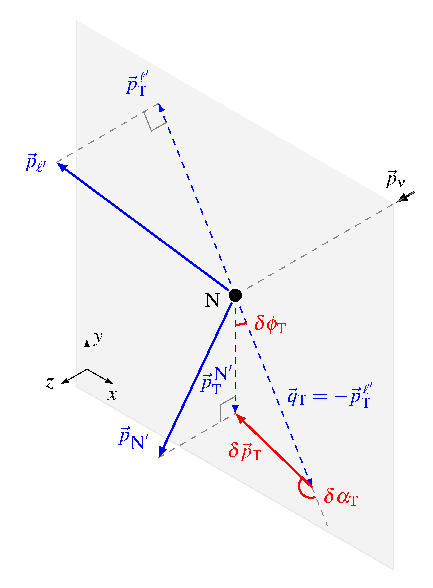
\includegraphics[width=0.35\textwidth]{figures/stki.eps}
            \caption{\label{fig:stki} Schematic illustration of the TKI variables. Diagram taken from Ref.~\cite{Lu:2015tcr}.} 
        \end{figure}
    
       The TKI variables are shown in Fig.~\ref{fig:stki}. They are cleverly constructed such that they are most sensitive to IS and FSI. 
       In the simplest case, there are only two final particles after the neutrino-nucleon interaction, a muon and a proton. 
       If the initial momentum of the struck nucleon has no component transverse to the neutrino's incoming direction, the products, i.e. the muon and the proton, should not have a net transverse component either, unless the struck nucleon has a non-zero initial transverse component or the final particles have undergone FSI.
       Suppose there is no FSI, the net transverse component, $\dpt$, corresponds exactly to the magnitude of the transverse component of the struck nucleon, and the angle, $\dat$, represents the direction of the initial nucleon motion projected on the transverse plane. 
       Assuming the nucleons are moving isotropically, the $\dat$ distribution should be flat. 
       All current nuclear models do not have a preferential direction for initial nuclear motion, so it is only natural to assume the nucleons move in random directions. 
       Thus, the deviation from flatness for $\dat$ can only be due to FSI, thereby making it an excellent probe for FSI. 
       As for $\dpt$, it reflects the magnitude of the initial nucleon momentum transverse to the neutrino direction compounded by FSI. 
       Furthermore, if the nucleus is assumed to be at rest and no other particles are knocked out other than the muon and the proton, the initial nucleon momentum, $\pn$, can also be derived following the steps outlined in \cite{pnpaper}. 
    

    \subsection{TKI in $\numucczpiop$ selection}
    
        To make a measurement of the TKI variable, an event selection needs to be made.
        At ND280, the protons from the primary neutrino interaction do not travel far and are usually contained in SFGD. 
        Hence, the $\numucczpiop$ presented in this section refers to the sample with the primary muon travelling into the vertical TPC and the proton contained in SFGD. 
        
        This $\numucczpiop$ is made by requiring the presence of exactly one contained SFGD proton on top of the $\numucc$-inclusive selection. 
        The proton momentum reconstruction resolution in this sample is about $3.5\%$, which is considerably high. 
        However, as shown in Fig.~\ref{fig:pn-res-bfESC}, there are a considerable portion of events with under-estimated $\pn$, which is largely removed after ESC selection, as shown in Fig.~\ref{fig:pn-res-afESC}.
        This strongly demonstrates the necessity of using ESC selection for TKI measurements.

        \begin{figure}[!htb] 
           \centering
           \begin{subfigure}{0.45\textwidth}
                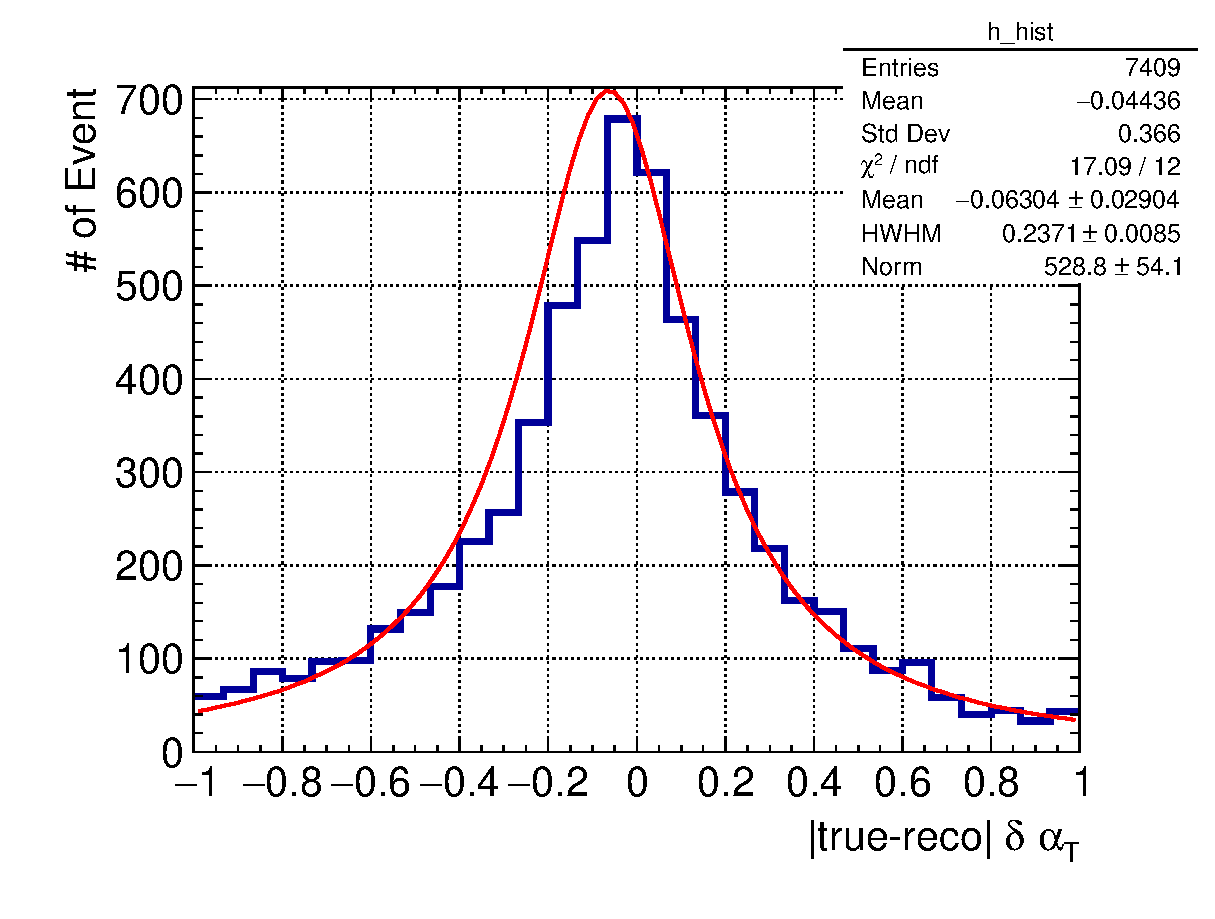
\includegraphics[width=\textwidth]{figures/dalphat_rat_hist_al13.eps}
                \caption{$\dat$ resolution before ESC selection.}
                \label{fig:dat-res-bfESC}
           \end{subfigure}
           \begin{subfigure}{0.45\textwidth}
                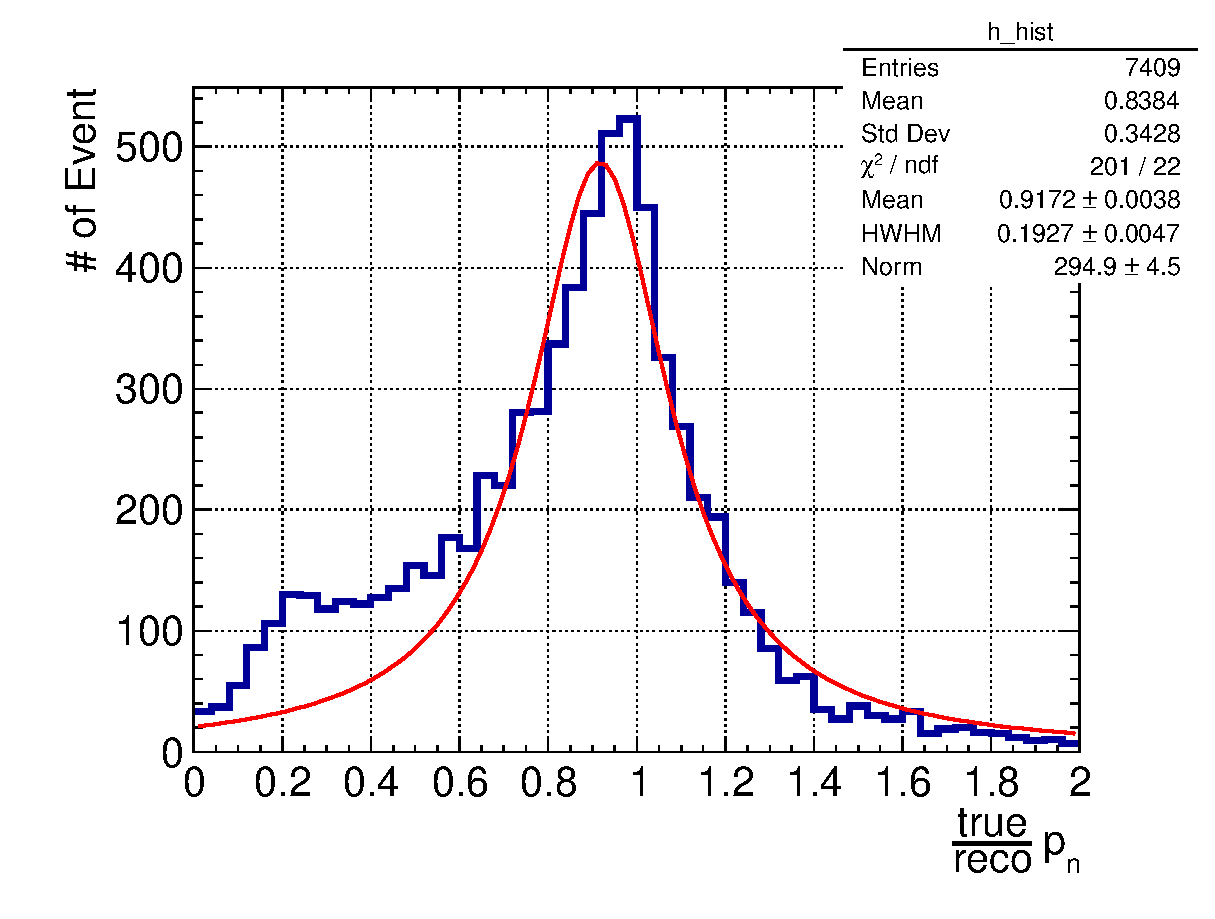
\includegraphics[width=\textwidth]{figures/pn_rat_hist_al13.eps}
                \caption{$\pn$ resolution before ESC selection.}
                \label{fig:pn-res-bfESC}
           \end{subfigure}
           \\
            \begin{subfigure}{0.45\textwidth}
                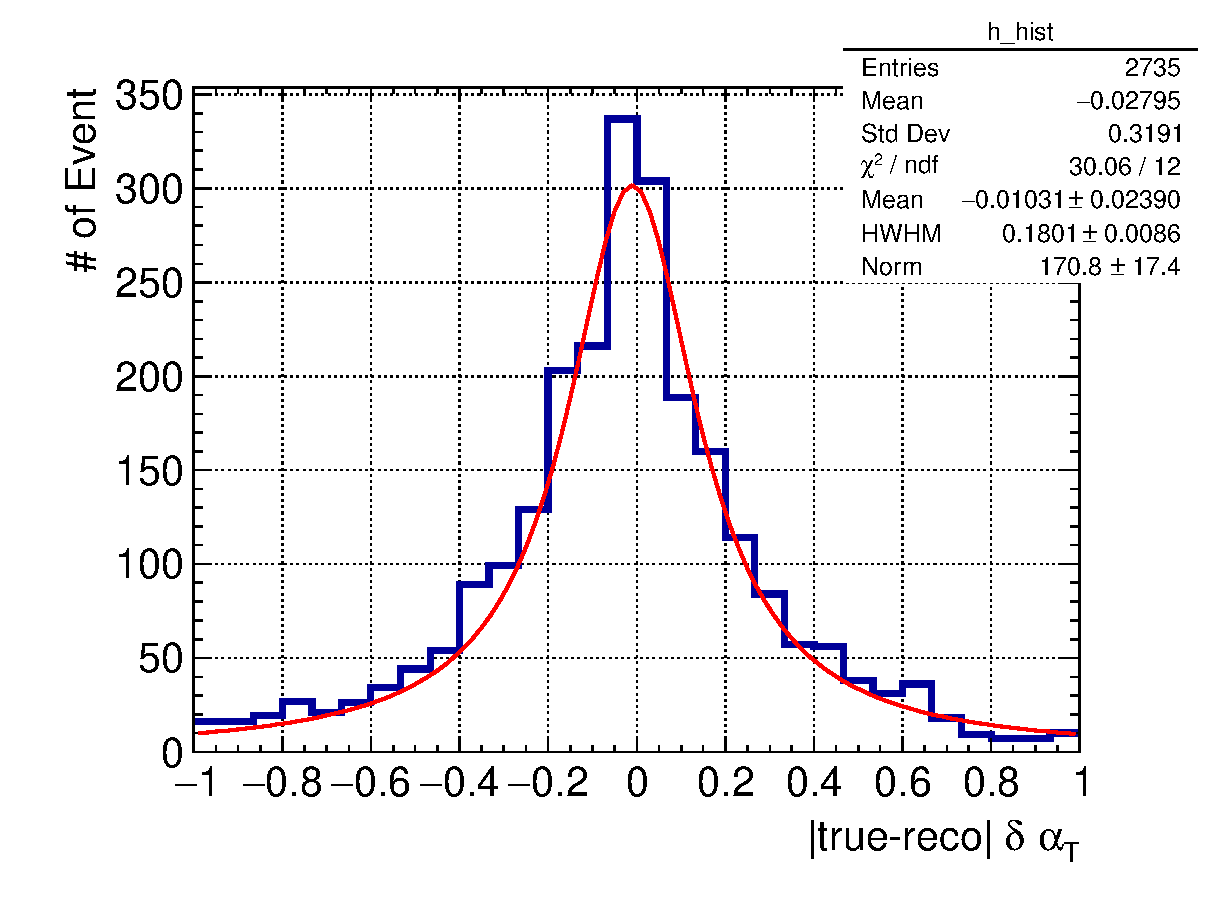
\includegraphics[width=\textwidth]{figures/dalphat_rat_hist_al14.eps}
                \caption{$\dat$ resolution after ESC selection.}
                \label{fig:dat-res-afESC}
           \end{subfigure}
           \begin{subfigure}{0.45\textwidth}
                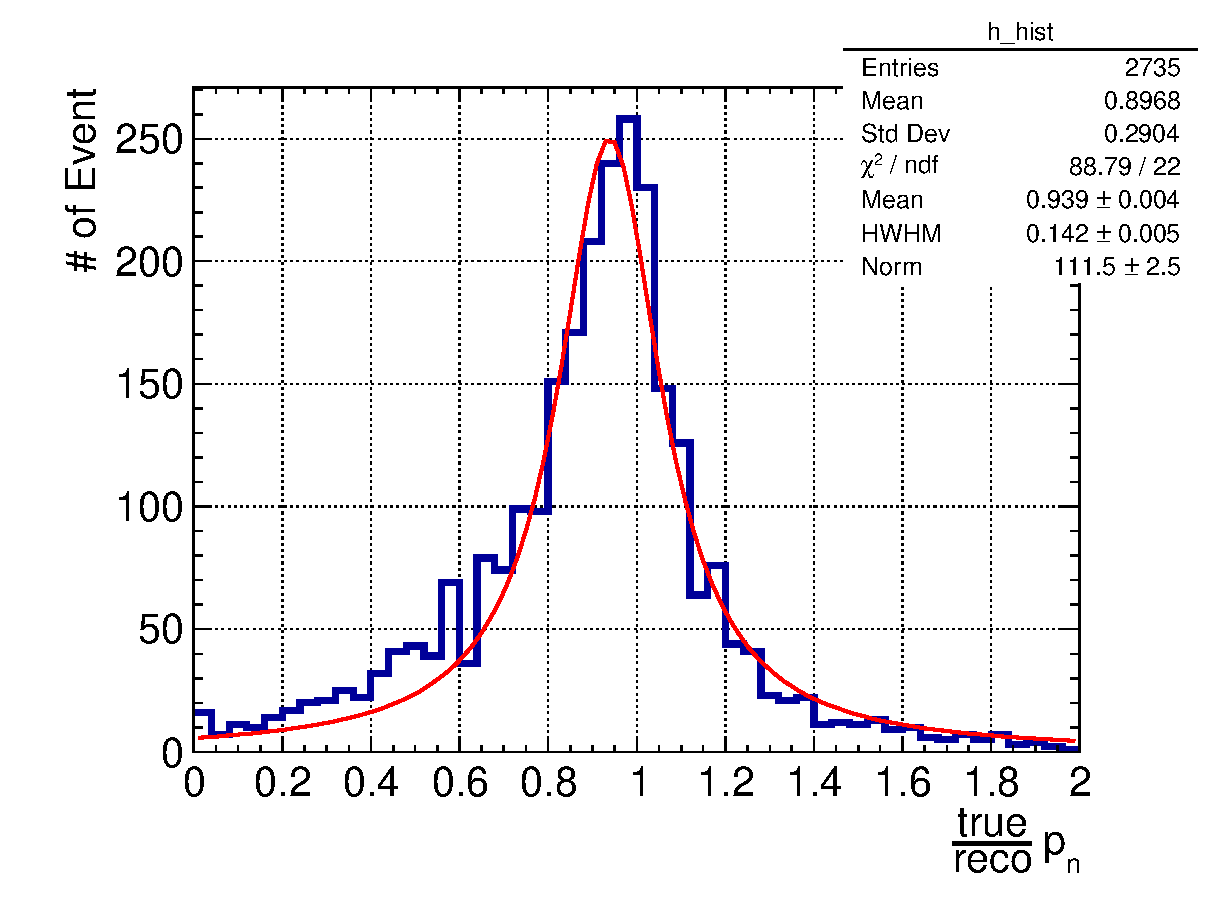
\includegraphics[width=\textwidth]{figures/pn_rat_hist_al14.eps}
                \caption{$\pn$ resolution after ESC selection.}
                \label{fig:pn-res-afESC}
           \end{subfigure}
           \\
            \begin{subfigure}{0.45\textwidth}
                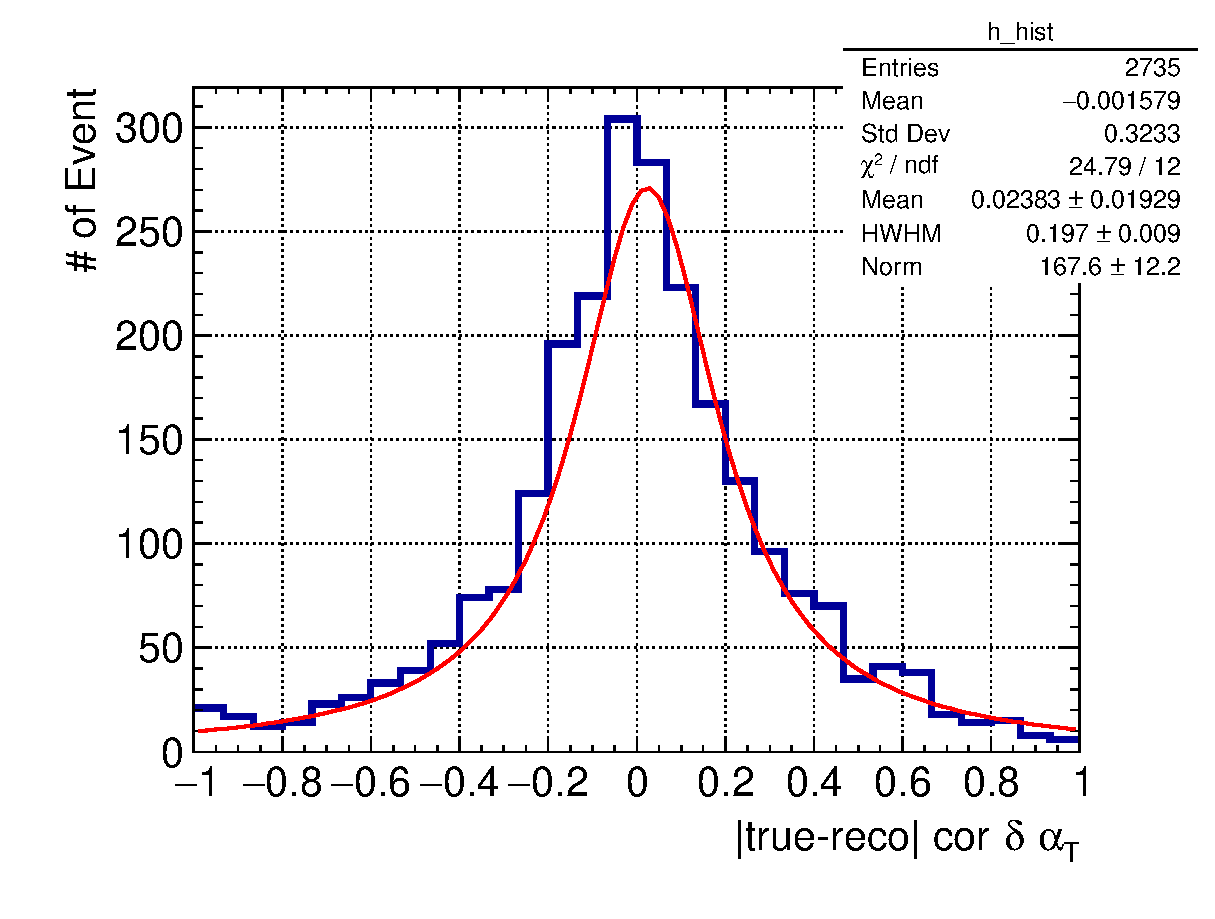
\includegraphics[width=\textwidth]{figures/cor_dalphat_rat_hist_al14.eps}
                \caption{$\dat$ resolution after $\pmut$ correction.}
                \label{fig:0pi-cordat}
           \end{subfigure}
           \begin{subfigure}{0.45\textwidth}
                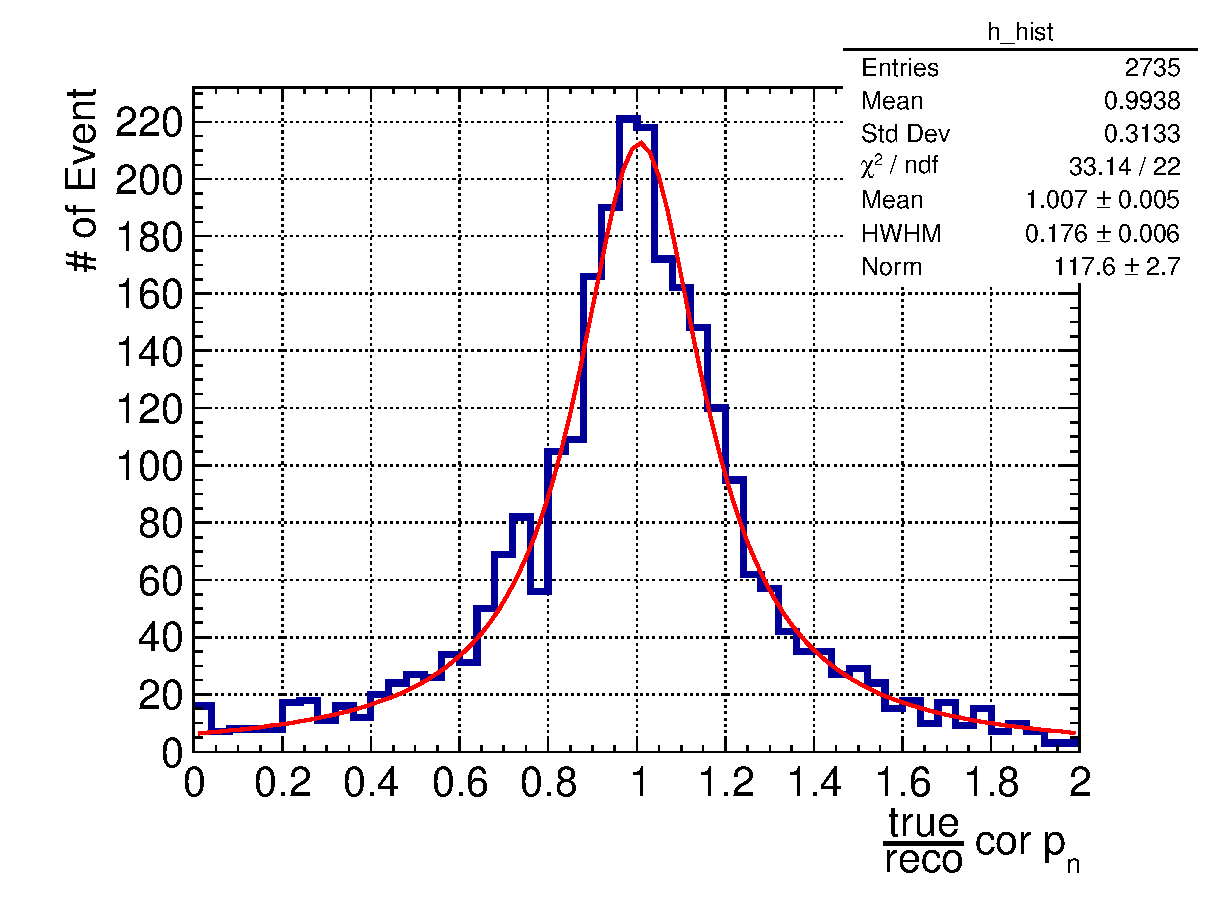
\includegraphics[width=\textwidth]{figures/cor_pn_rat_hist_al14.eps}
                \caption{$\pn$ resolution after $\pmut$ correction.}
                \label{fig:0pi-corpn}
           \end{subfigure}
           \caption{TKI reconstruction results.}
           \label{fig:tki-res-bfafESC}
        \end{figure}

        With the ESC selection, the resolution of $\dat$ and $\pn$ has improved considerably from $0.23$ to $0.18~\textrm{rad}$ and from $19.3\%$ to $14.2\%$ respectively. Moreover, the fitted bias has decreased from $-0.06$ to $-0.01~\textrm{rad}$ and from $1-0.917=0.083$ to $1-0.939=0.061$ for $\dat$ and $\pn$ respectively.  

        As pointed out in Ref.~\cite{Lu:2016mjf}, the ESC selection might lead to a bias in the particle transverse momentum. 
        Such transverse bias would have to be checked after the ESC selection and, if any, corrected for better TKI measurement. 
        The results of the bias check are summarised in Fig.~\ref{fig:0piptbiascheck}. 
        There is no transverse bias for proton as shown in Fig.~\ref{fig:0pi-prpt-bias}, while there is a clear bias in muon $\pt$ for $0.5<\pmut<1.1~(\gevc)$. 
        It is further checked that this bias is not due to a bias in the angle reconstruction, as shown in Fig.~\ref{fig:0pi-mutheta-bias}.
        Thus, a correction is directly applied to $\pmut$ within the specified range, and the corrected $\pmut$ is shown in Fig.~\ref{fig:cormupt}.

       \begin{figure}[!htb]
           \centering
           \begin{subfigure}{0.3\textwidth}
                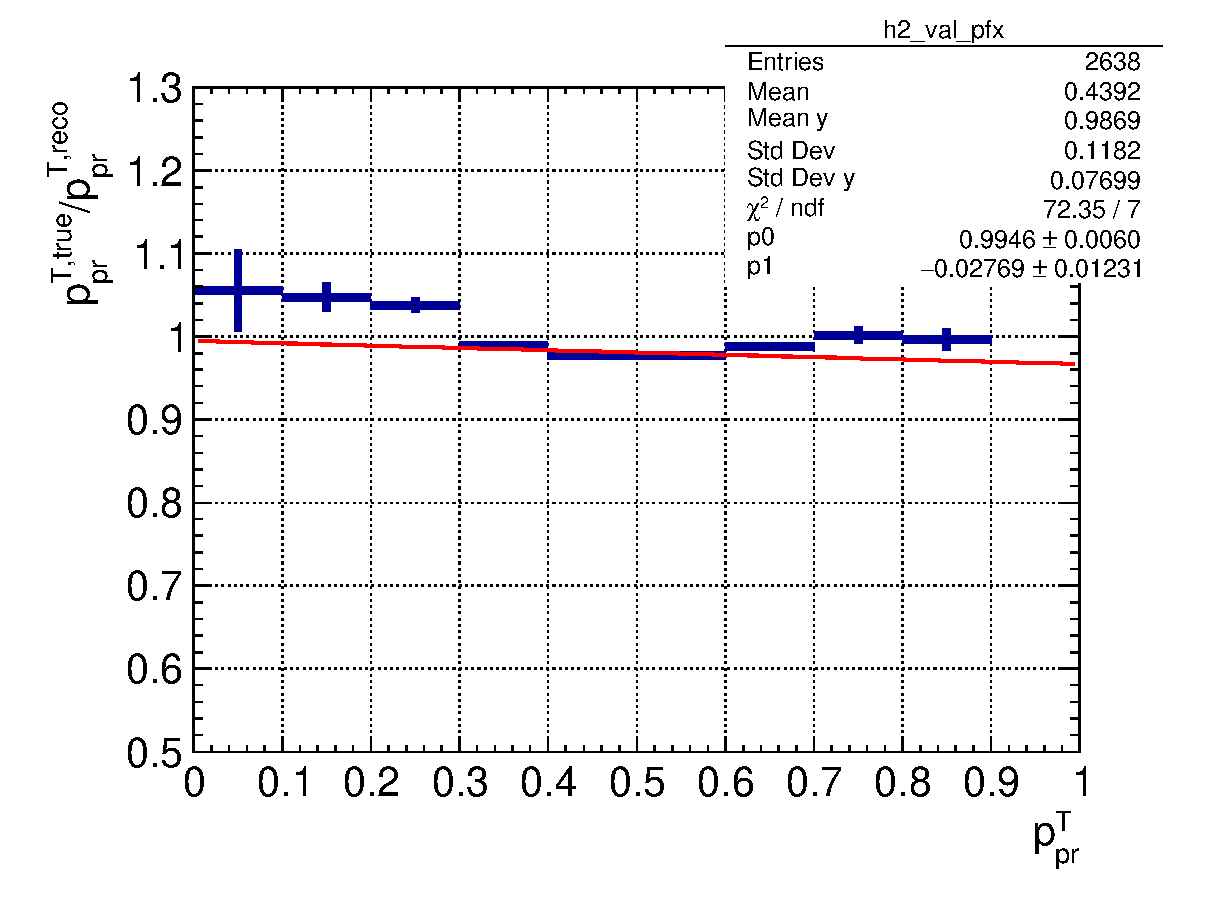
\includegraphics[width=\textwidth]{figures/pr_pt_vs_pr_pt_bias_hist2d_al14.eps}
                \caption{Proton transverse bias.}
                \label{fig:0pi-prpt-bias}
           \end{subfigure}
           \begin{subfigure}{0.3\textwidth}
                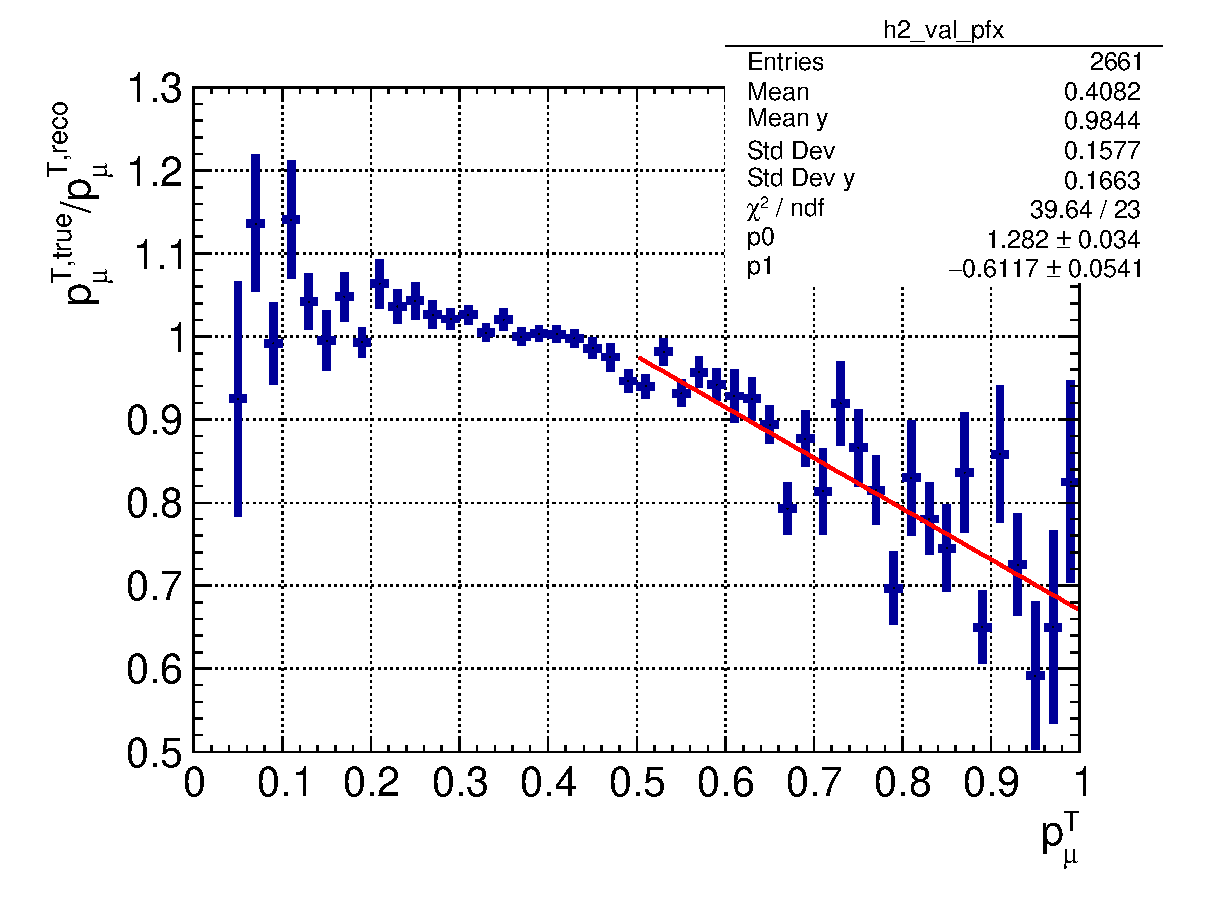
\includegraphics[width=\textwidth]{figures/mu_pt_vs_mu_pt_bias_hist2d_al14.eps}
                \caption{Muon transverse bias.}
                \label{fig:0pi-mupt-bias}
           \end{subfigure}
           \begin{subfigure}{0.3\textwidth}
                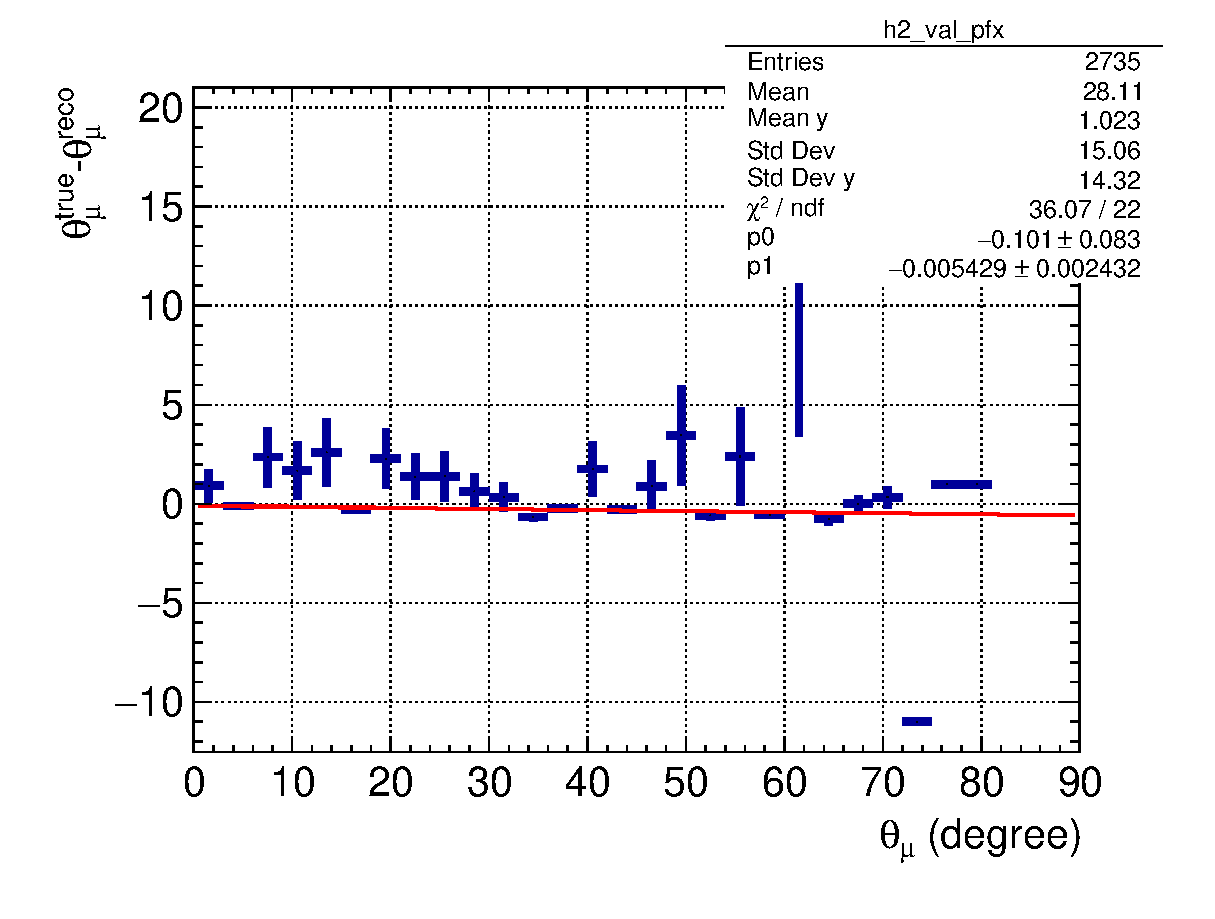
\includegraphics[width=\textwidth]{figures/theta_mu_vs_theta_mu_res_hist2d_al14.eps}
                \caption{Muon theta bias.}
                \label{fig:0pi-mutheta-bias}
           \end{subfigure}
           \caption{Transverse bias check after ESC selection.}
           \label{fig:0piptbiascheck}
        \end{figure}
            
        \begin{figure}[!htb] 	
            \centering 		
            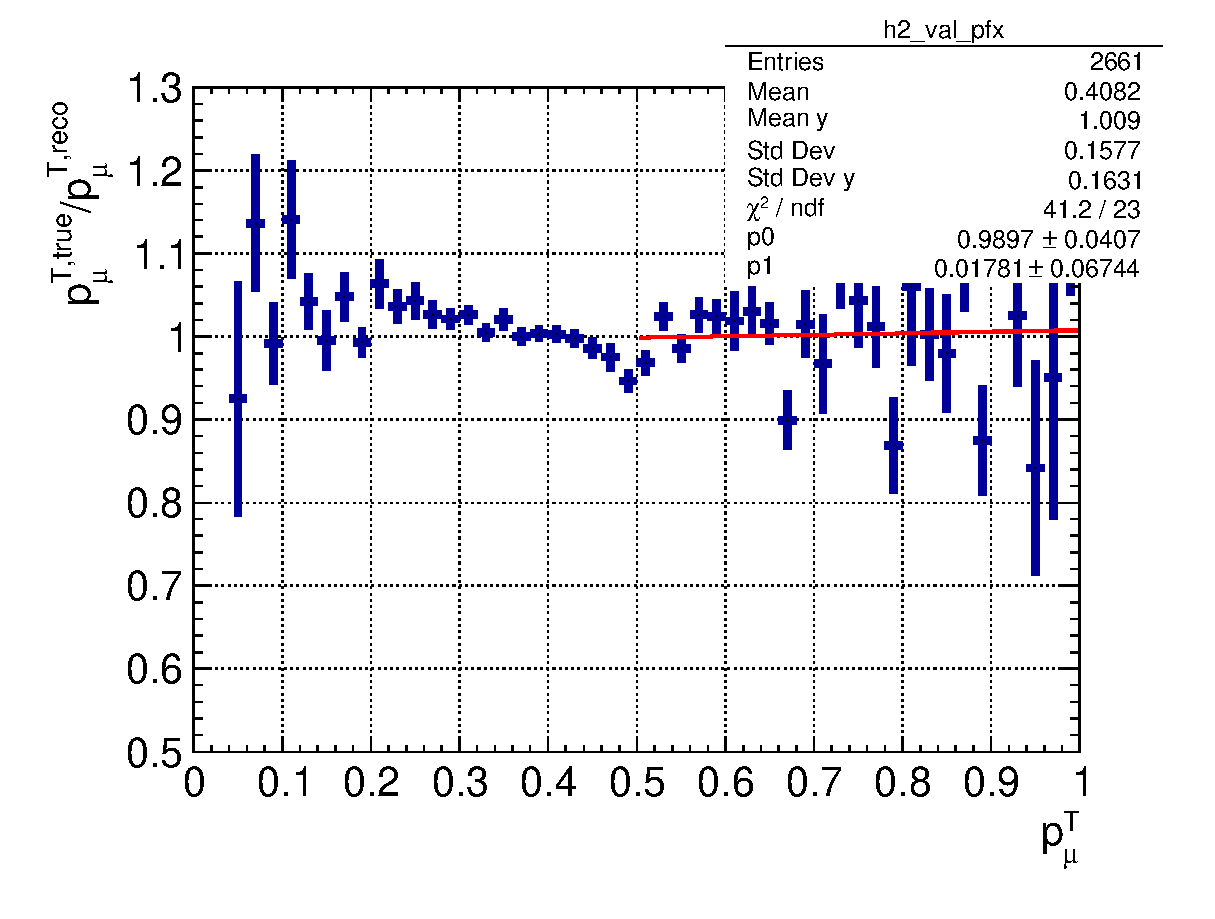
\includegraphics[width=0.35\textwidth]{figures/mu_pt_vs_cor_mu_pt_bias_hist2d_al14.eps}
            \caption{\label{fig:cormupt} Corrected $\pmut$.} 
        \end{figure}

        The impact of the $\pmut$ correction on the TKI variables are shown in Fig.~\ref{fig:0pi-cordat} and Fig.~\ref{fig:0pi-corpn}. The resolutions remain similar, while the bias in $\pn$ has significantly reduced from $6.1\%$ to $0.7\%$.

    \subsection{\label{sec:1pi-tki} TKI in $\numuccopiop$ selection}

    As I have the $\numuccopi$ selection along with the pion trackless reconstruction, it is straightforward to select a $\numuccopiop$ sample by adding an extra step of requiring exactly one SFGD contained proton that passes the ESC selection. 
    The $\pt$ biases are checked for all three particles and no biases are observed. Hence, the final TKI reconstruction results are given in Fig.~\ref{fig:1pi-tki-res}. Both $\dat$ and $\pn$ have minimal fitted bias, $-0.02~\textrm{rad}$ for $\dat$ and about $2\%$ for $\pn$. While the $\dat$ has a slightly worse resolution, $0.24~\textrm{rad}$, than that in $\numucczpiop$, $\pn$ has a better resolution, $12\%$. 
    
   \begin{figure}[!htb] 
       \centering
       \begin{subfigure}{0.45\textwidth}
            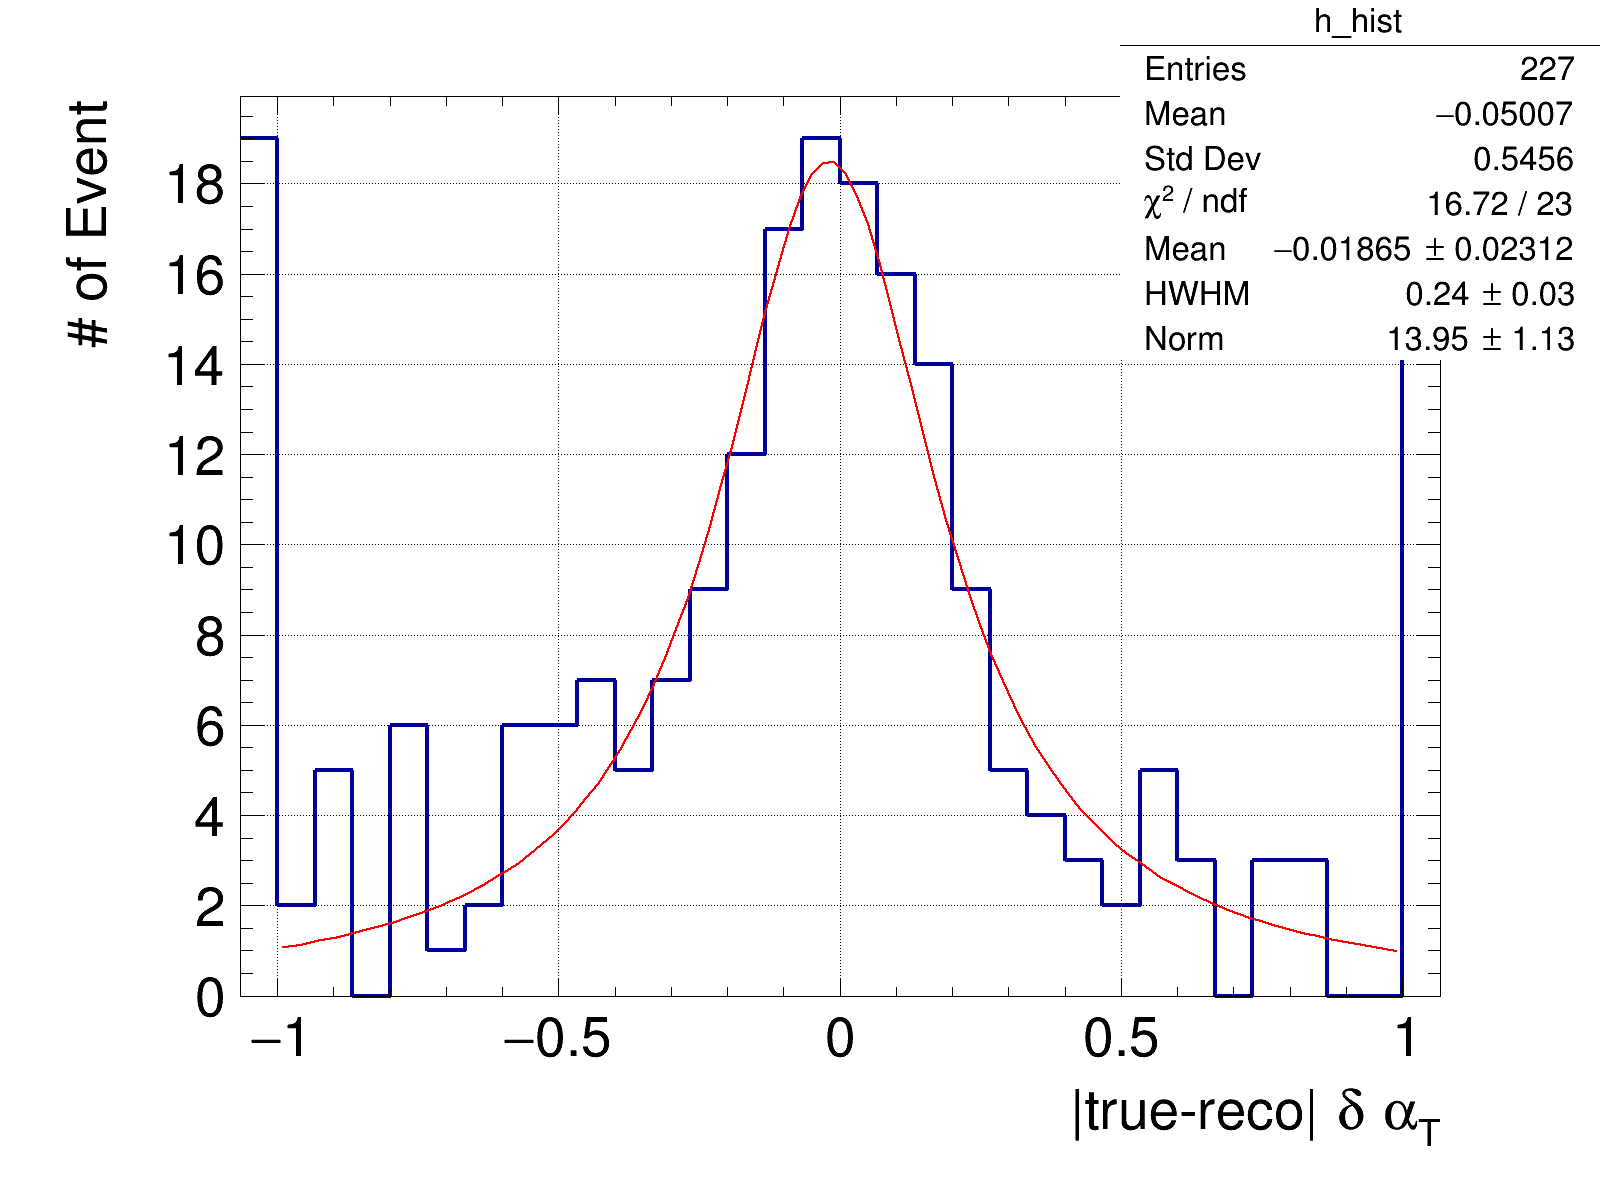
\includegraphics[width=\textwidth]{figures/SFGpTPCmu_dalphat_rat_hist_al14.png}
            \caption{$\dat$ resolution.}
            \label{fig:1pi-dat-res}
       \end{subfigure}
       \begin{subfigure}{0.45\textwidth}
            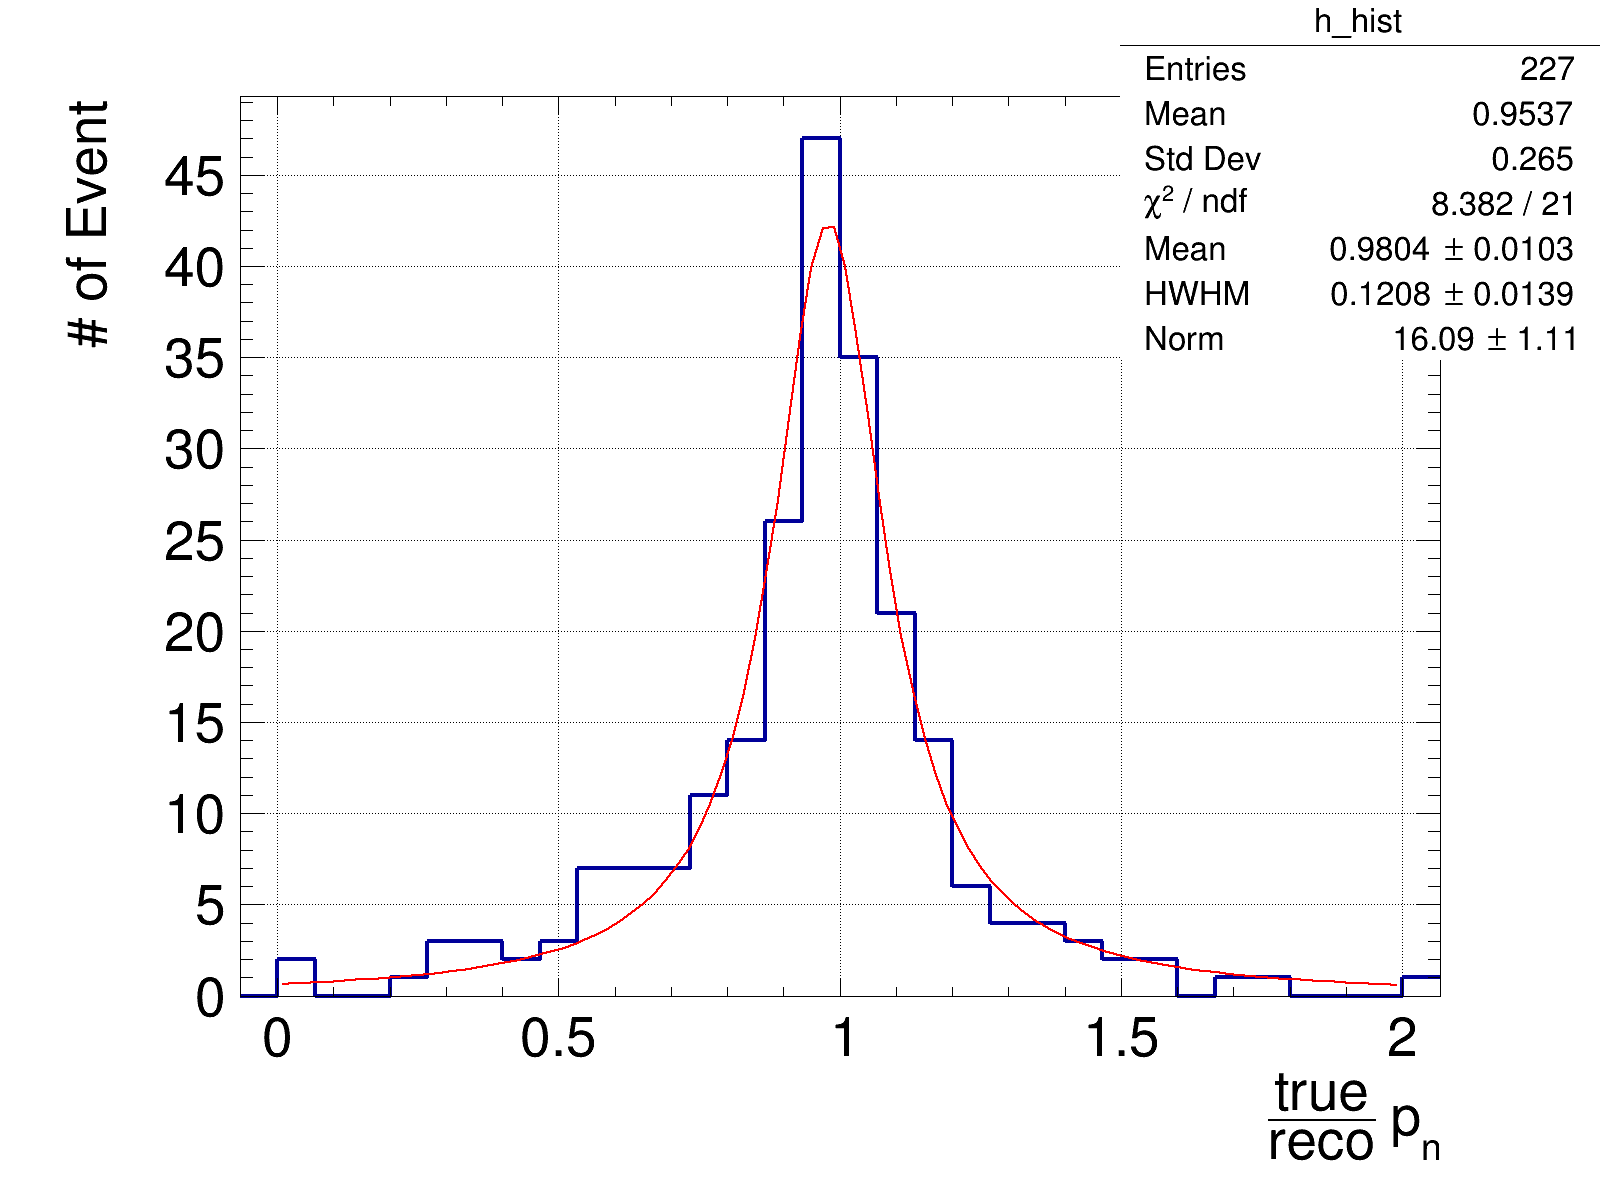
\includegraphics[width=\textwidth]{figures/SFGpTPCmu_pn_rat_hist_al14.png}
            \caption{$\pn$ resolution.}
            \label{fig:1pi-pn-res}
       \end{subfigure}
       \caption{TKI reconstruction results.}
       \label{fig:1pi-tki-res}
    \end{figure}

    In additional to the single transverse variables presented above, the $\numuccopiop$ sample can also be used to measure the double transverse variable, $\dptt$, the net momentum transverse to both the neutrino momentum and the muon momentum,
    Without FSI, $\dptt$ should be $0$. This special property can be exploited to select $\nu$-H events amidst $\nu$-C events as suggested in Ref.~\cite{dpttpaper}. 
    Hence, the main figure of merit for $\dptt$ measurement is the width of its distribution for $\nu$-H events, where the hydrogen events are picked by an additional check on the MC truth information.
    As shown in Fig.~\ref{fig:dptt-hist}, the fitted half width is about $12~\mevc$, which is significantly improved compared to $21~\mevc$, the pre-upgrade ND280 result \cite{dpttpaper}.

    \begin{figure}[!htb] 
        \centering 		
        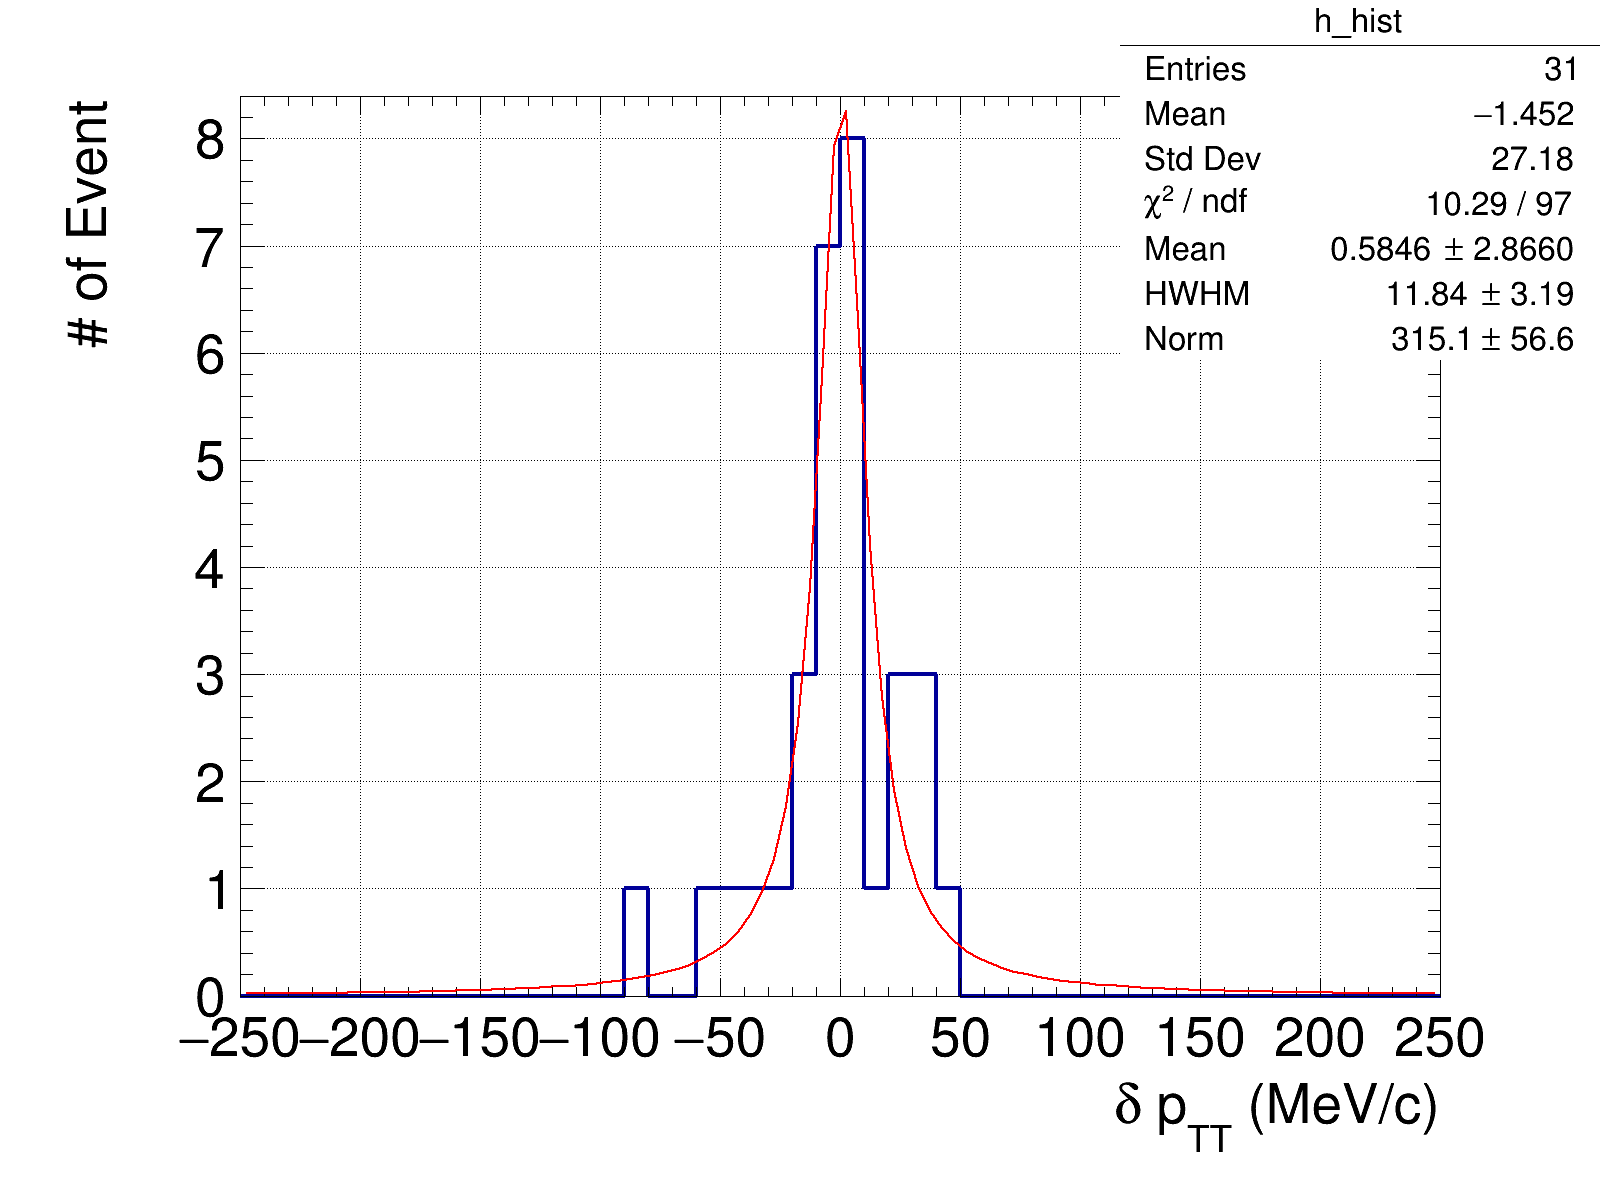
\includegraphics[width=0.35\textwidth]{figures/SFGpTPCmu_dptt_hist_al15_H_bin100_range500_Lfit.png}
        \caption{\label{fig:dptt-hist} $\dptt$ distribution for $\nu$-H events.} 
    \end{figure}



\begin{savequote}[8cm]
\textlatin{Neque porro quisquam est qui dolorem ipsum quia dolor sit amet, consectetur, adipisci velit...}

There is no one who loves pain itself, who seeks after it and wants to have it, simply because it is pain...
  \qauthor{--- Cicero's \textit{de Finibus Bonorum et Malorum}}
\end{savequote}

\chapter{\label{ch:6-hnl}HNL} 

\minitoc


    \subsection{Heavy Neutral Leptons (HNL)}
    \subsubsection{Background}
        As a detailed review of HNL would exceed the scope of this report, only a highly simplified introduction to HNL is given here. 
        The origin of the neutrino mass is still a mystery. 
        One intuitive solution is to extend the neutrino family to include heavy members, which mix with the existing SM neutrinos via an extended PMNS matrix and give them the small masses observed via the see-saw mechanism~\cite{Abada_2007}. 
        As they mix the SM neutrinos, they could be produced in the intense neutrino beam in the long-baseline neutrino experiments, so the near detector of these experiments is the best place to look for HNL. 
        The signal comes from HNL decays, some of which are distinct from SM neutrino interactions. 
        Previously, T2K has searched for HNL~\cite{T2K:2019jwa} using the TPCs, a combined volume of about $7~\textrm{m}^3$, in ND280. As 
        the ND280 upgrade replaces the P0D with SFGD and HATPC, a combined volume of $8~\textrm{m}^3$, which are much better trackers than the P0D, they could be used in an HNL search as well, thereby improving the overall sensitivity. 

        To perform such an HNL search, a complicated chain of simulations is required, including the generation of an HNL flux based on the SM neutrino flux, the propagation of HNL and the decay of HNL. 
        The previous T2K search was based on a dedicated tool-set, \code{nd280HNLSim}, which was built only to search for $N\rightarrow l + \pi$ decay channels, where $l$ is a lepton. 
        It would require a large amount of efforts to extend it to include other production and decay channels. 
        Hence, I adapt the recently published general HNL package, \code{BeamHNL}~\cite{Plows:2022gxc}, to the T2K ND280 simulation to evaluate the sensitivity improvement brought by the upgrade.

    \subsubsection{Implementation}
        The simulation of production and decay of HNL by \code{BeamHNL} is performed in several steps.
        As \code{BeamHNL} aims to be a cross-experiment package, it requires a standardised flux input, the \code{dk2nu} format. 
        The \code{dk2nu} file is a simple flattree root file that needs to contain the minimally sufficient information for \code{BeamHNL} to work.
        As the T2K flux is available in its specific format, a conversion is required. 
        The required \code{dk2nu} variables and the required conversion from corresponding variables in a T2K flux file are given in Appendix~\ref{sec:app-hnl-dk2nu}.

        With this input, desired channels of HNL production can then be performed with a few additional parameters specified by a configuration \code{xml} file, \code{CommonHNL.xml}, inside the \code{GENIE} configuration directory. 
        These parameters are experiment-specific, so they need to be set by the user. Details of how each parameter is set specific to the T2K ND upgrade are provided in the Appendix~\ref{sec:app-hnl-input}. 

        Before running subsequent steps, we validate that if we feed the T2K \code{dk2nu} file to \code{BeamHNL} and set the HNL mass, $\mn$, to a small value, such as $1~\kev$, the output HNL flux should closely mimic the SM flux. 
        The result is shown in Fig.~\ref{fig:hnl-fluxes}, which shows that the pink dash line ($\mn=1~\kev$) overlaps closely with the black solid line, which plotted directly from the T2K input flux.  
        \begin{figure}[!htb] 
            \centering 		
            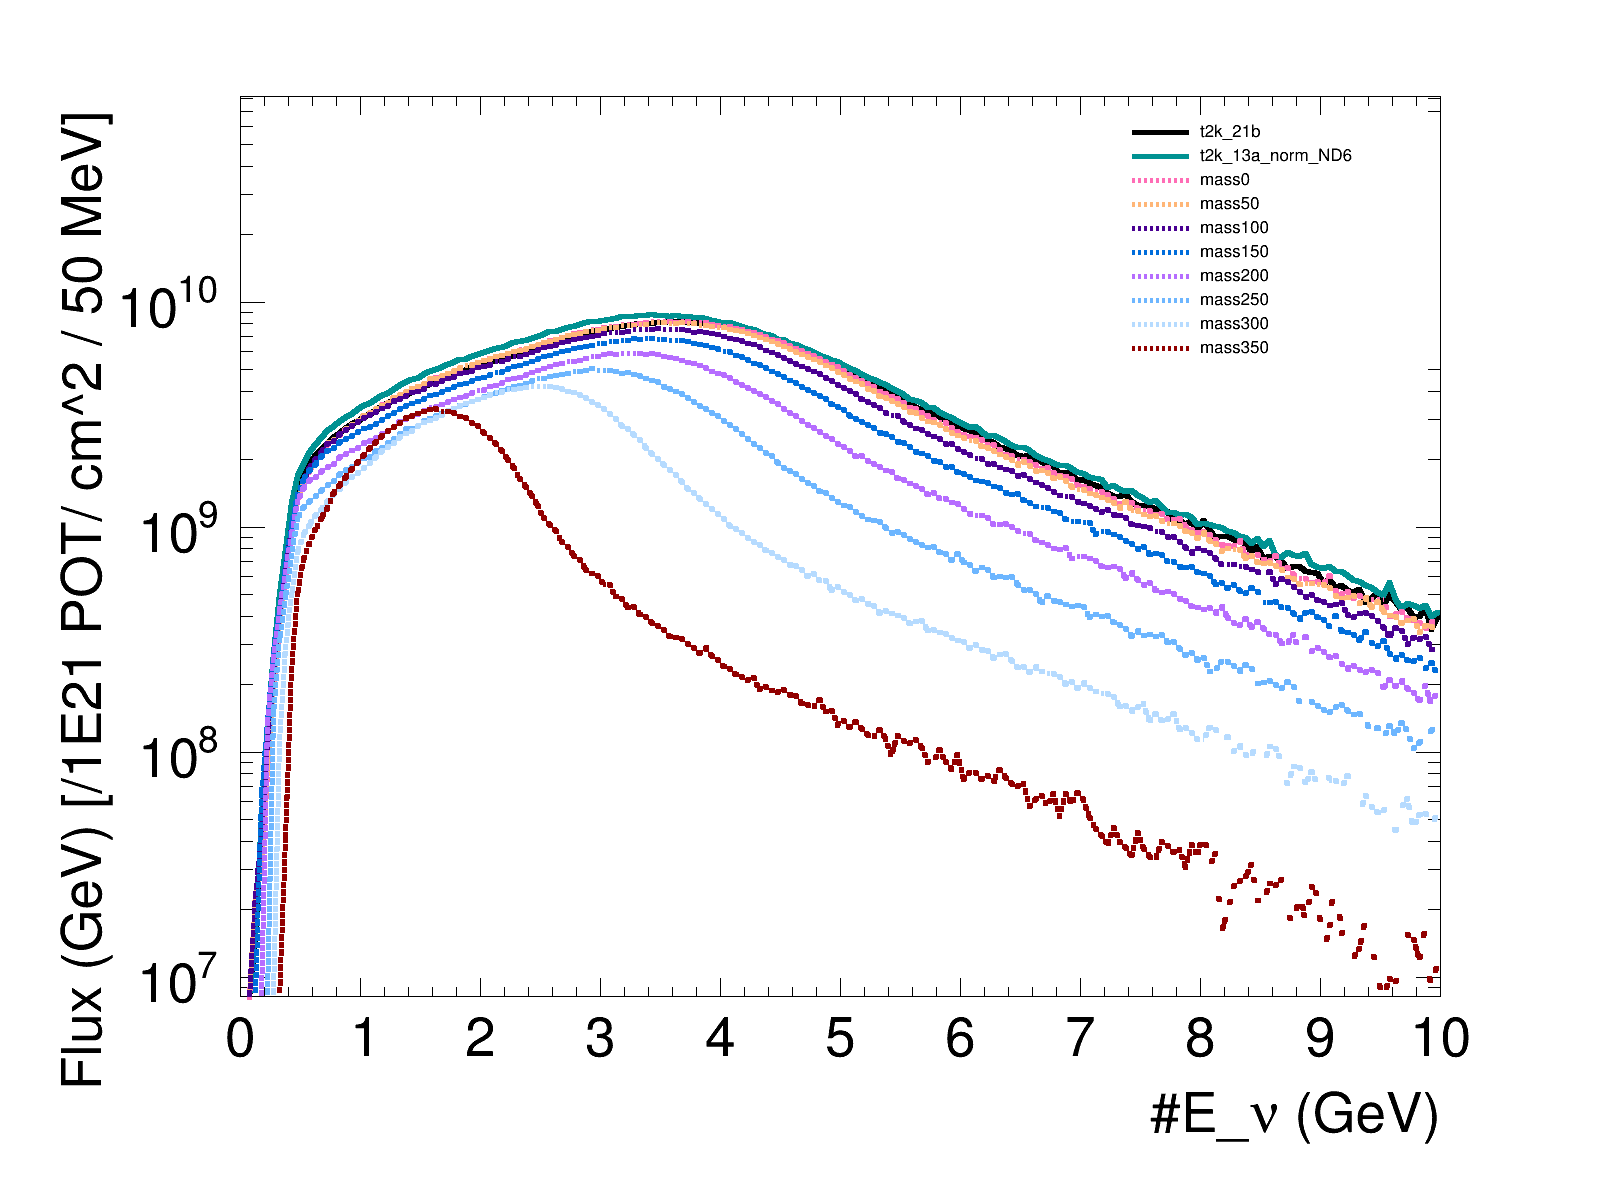
\includegraphics[width=0.45\textwidth]{figures/hnl_fluxes.png}
            \caption{\label{fig:hnl-fluxes} HNL fluxes produced by \code{BeamHNL} for different $M_N$. The solid lines are directly plotted from T2K input flux files, one with version ``13a'' and another with ``21b''. The dash lines are \code{BeamHNL} outputs for different $\mn$.} 
        \end{figure}
        After the validation, the HNL mass is then set to target values, e.g. $300~\mev$, to generate HNL events, which are then passed through the T2K simulation chain for selection development. 
        \begin{figure}[!htb] 
            \centering 		
            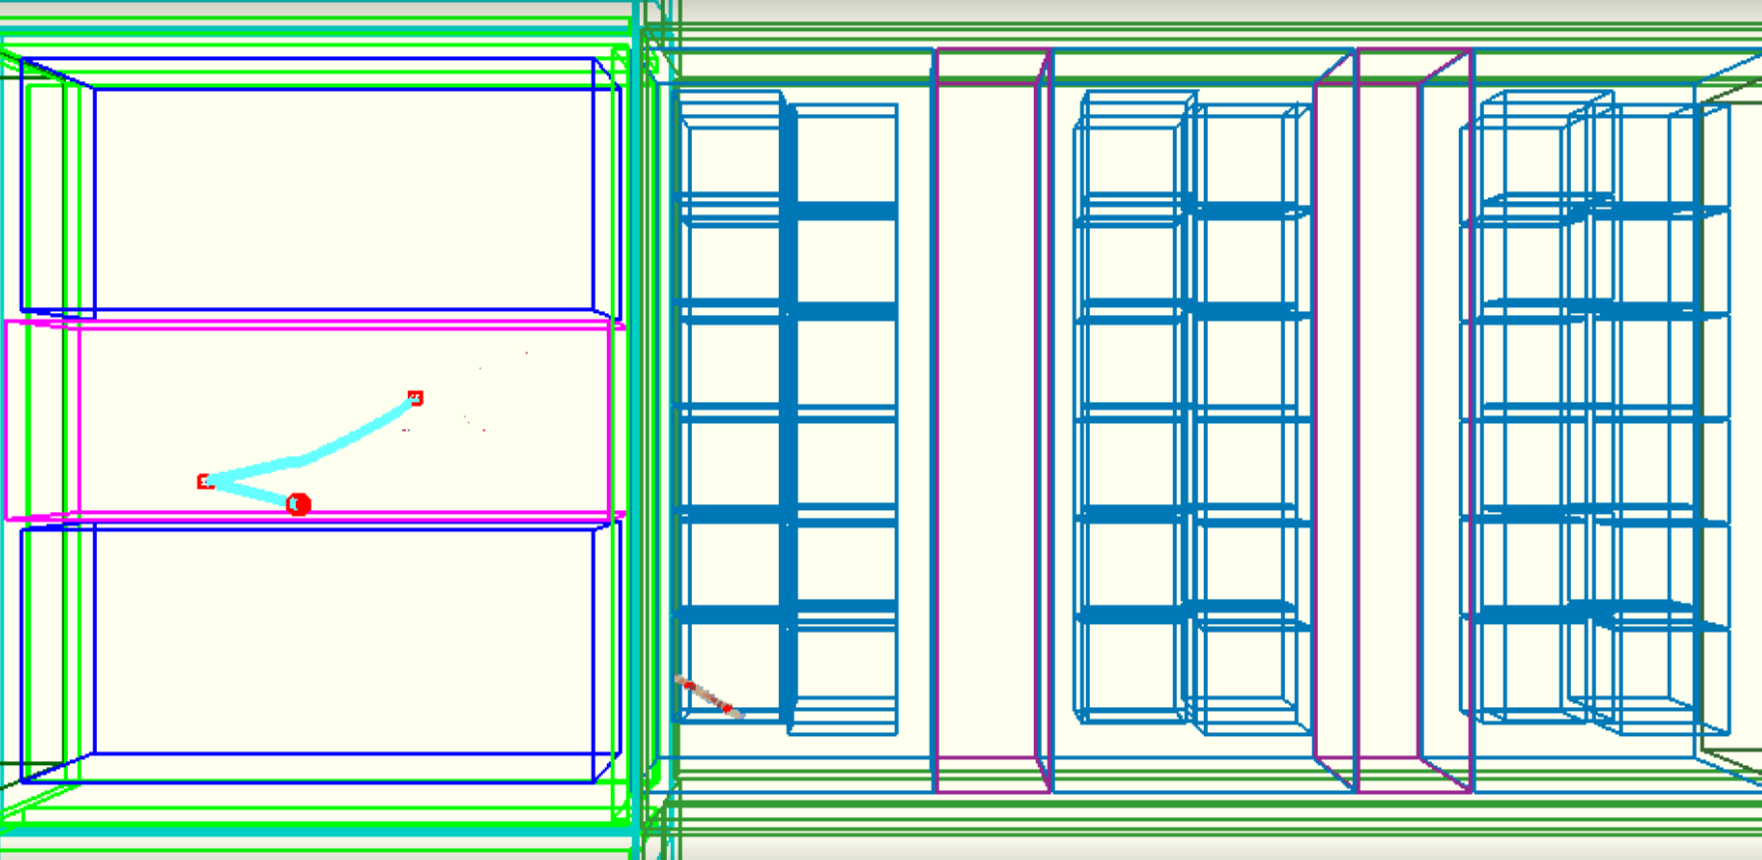
\includegraphics[width=0.45\textwidth]{figures/HNLEveDIs.png}
            \caption{\label{fig:hnl-evedis} A $N\rightarrow\mu+\pi$ event display in the upgraded ND280.} 
        \end{figure}

        It is natural to begin with the development of selecting the same signal channel as the previous T2K search to cross-validate before extending to more channels. Hence, I first developed the selection for the $N\rightarrow\mu+\pi$ channel. The steps are as follows:

        \begin{enumerate}
            \item \textbf{Basic T2K Event Quality Steps} 
            \item \textbf{Find SFGD Primary Vertex} 
            \item \textbf{No. of primary tracks cut} 
            \item \textbf{Escaping muon cut} 
            \item \textbf{One Trackless pion cut}
            \item \textbf{Kink cut}
            \item \textbf{$\mu$-$\pi$ angle and invariant cut}
            \item \textbf{$\mu$-$\pi$ $\dpt$ cut}
        \end{enumerate}

        \textbf{Basic T2K Event Quality Steps} - A quality check ensures the event contains at least $1$ reconstructed track.

        \textbf{Find SFGD Primary Vertex} - Find a primary vertex in SFGD. 
        As the primary vertex for an HNL event does not necessarily include a muon like in the $\numucc$ selection, a primary vertex should be identified independently from finding a primary muon. 
        All vertices are looped through to record the number of tracks connected to each vertex, $n_{ptrk}$ and the length of the longest track connected to each vertex, $L_{max}$. 
        The vertex with the longest $L_{max}$ is selected as the primary vertex. 
        If there is more than one such vertex, the vertex with the largest $n_{trk}$ is selected. 
        If there is still more than such one vertex, the vertex with the earliest time is selected.

        \textbf{No. of primary tracks cut} - As the target channel is $N\rightarrow\mu+\pi$, there should at most be two primary tracks. Hence, events with $n_{ptrk}>2$ are rejected.

        \textbf{Escaping muon cut} - A standard step to identify a muon escaping SFGD.

        \textbf{One Trackless pion cut} and \textbf{Kink cut} - They are the same as those in $\numuccopi$-Trackless, selecting a primary pion that has not undergone secondary interaction to ensure accurate reconstruction of its kinematics.

        \textbf{$\mu$-$\pi$ angle and invariant mass cut} - These are kinematic cuts exploiting the fact that the SM events with $1$ muon and $1$ pion are mostly resonance events that has one more proton than the HNL decay. 
        Due to the additional proton, the opening angle between the $\mu$ track and the $\pi$ track, $\tmupi$, can have large variations while that of an HNL decay would be more collimated. 
        Similarly, the invariant mass of the $\mu$-$\pi$ system, $\mmupi=(\pmu+\ppi)^2$ would have a larger range compared to the HNL, which centres around the input value, $300~\mev$ as shown in Fig.~\ref{fig:hnl-mmupi}.
        The stark contrast is apparent in Fig.~\ref{fig:mmupi-mupiang}, and to preserve the most number of HNL events, the specific cuts are: $30\degree<\tmupi<90\degree$ and $270~\mev<\mmupi<320~\mev$. 
        \begin{figure}[!htb]
           \centering
           \begin{subfigure}{0.45\textwidth}
                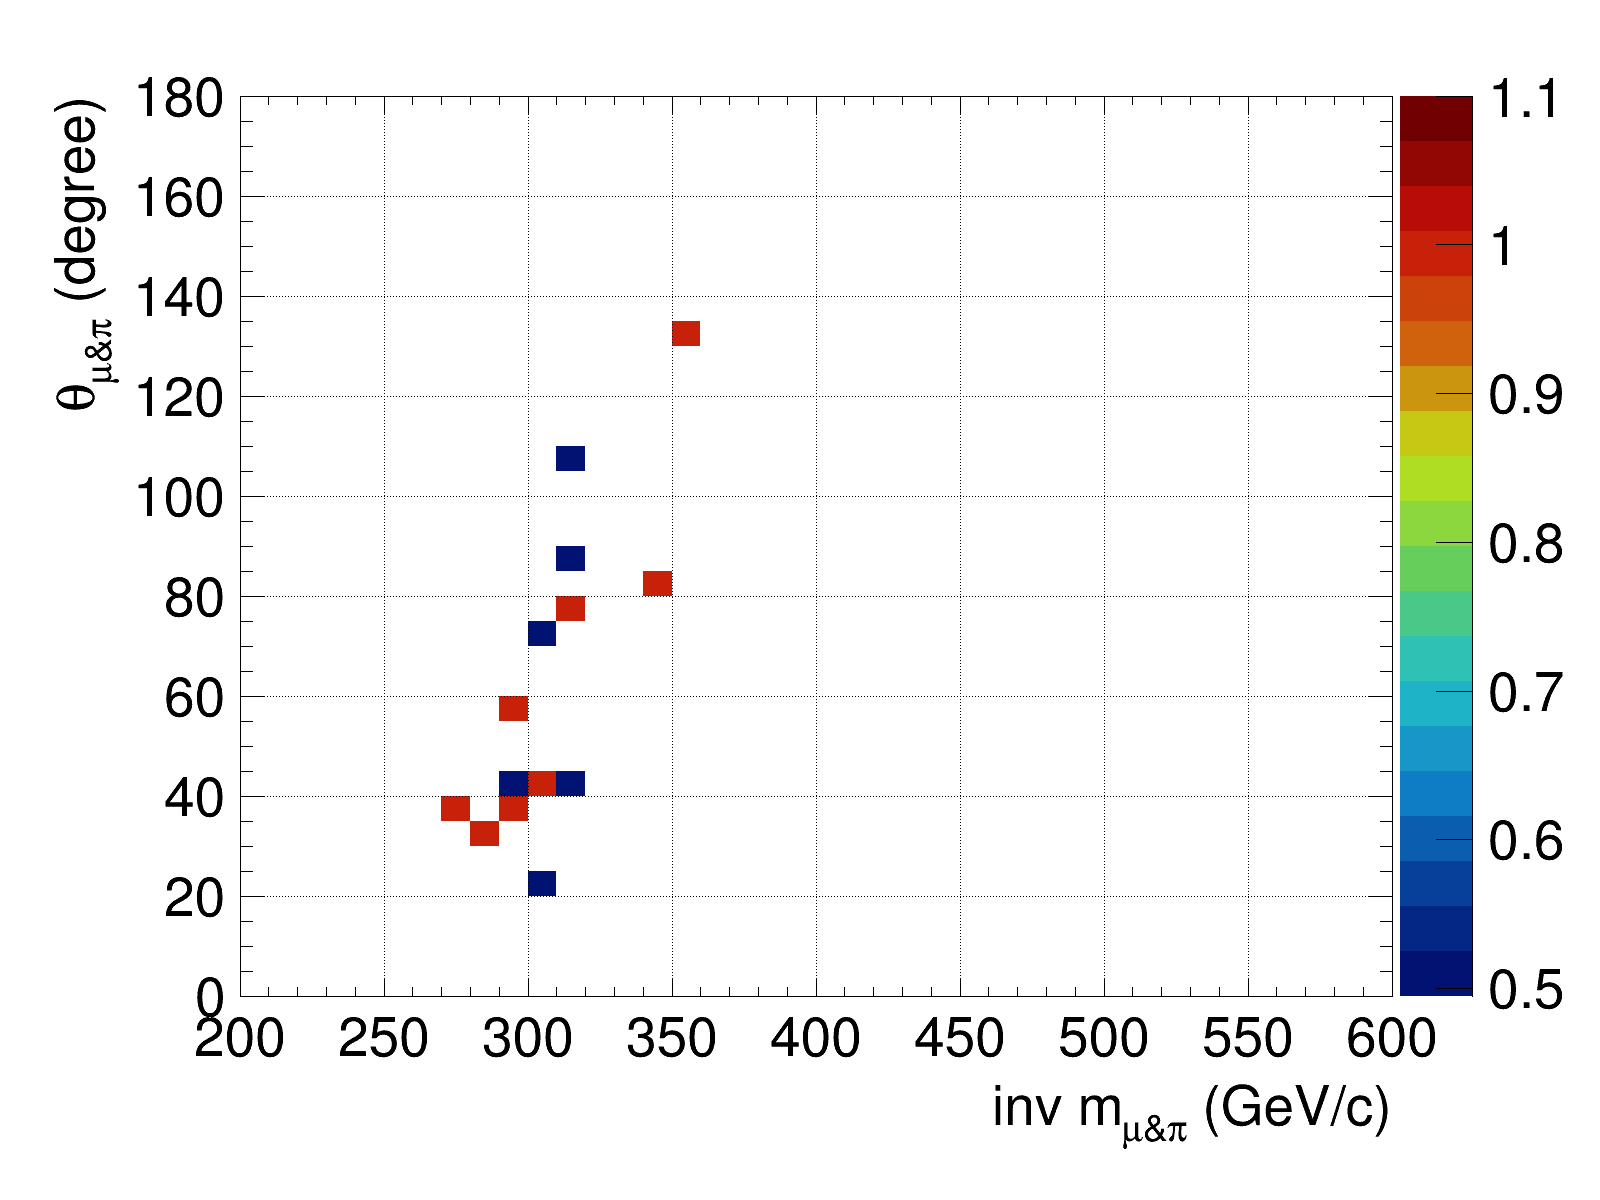
\includegraphics[width=\textwidth]{figures/hnl_sfgmu_mpinvm_colnor_vs_mpang_hist2d_al9_300.png}
                \caption{HNL.}
                \label{fig:hnl-mmupi}
           \end{subfigure}
           \begin{subfigure}{0.45\textwidth}
                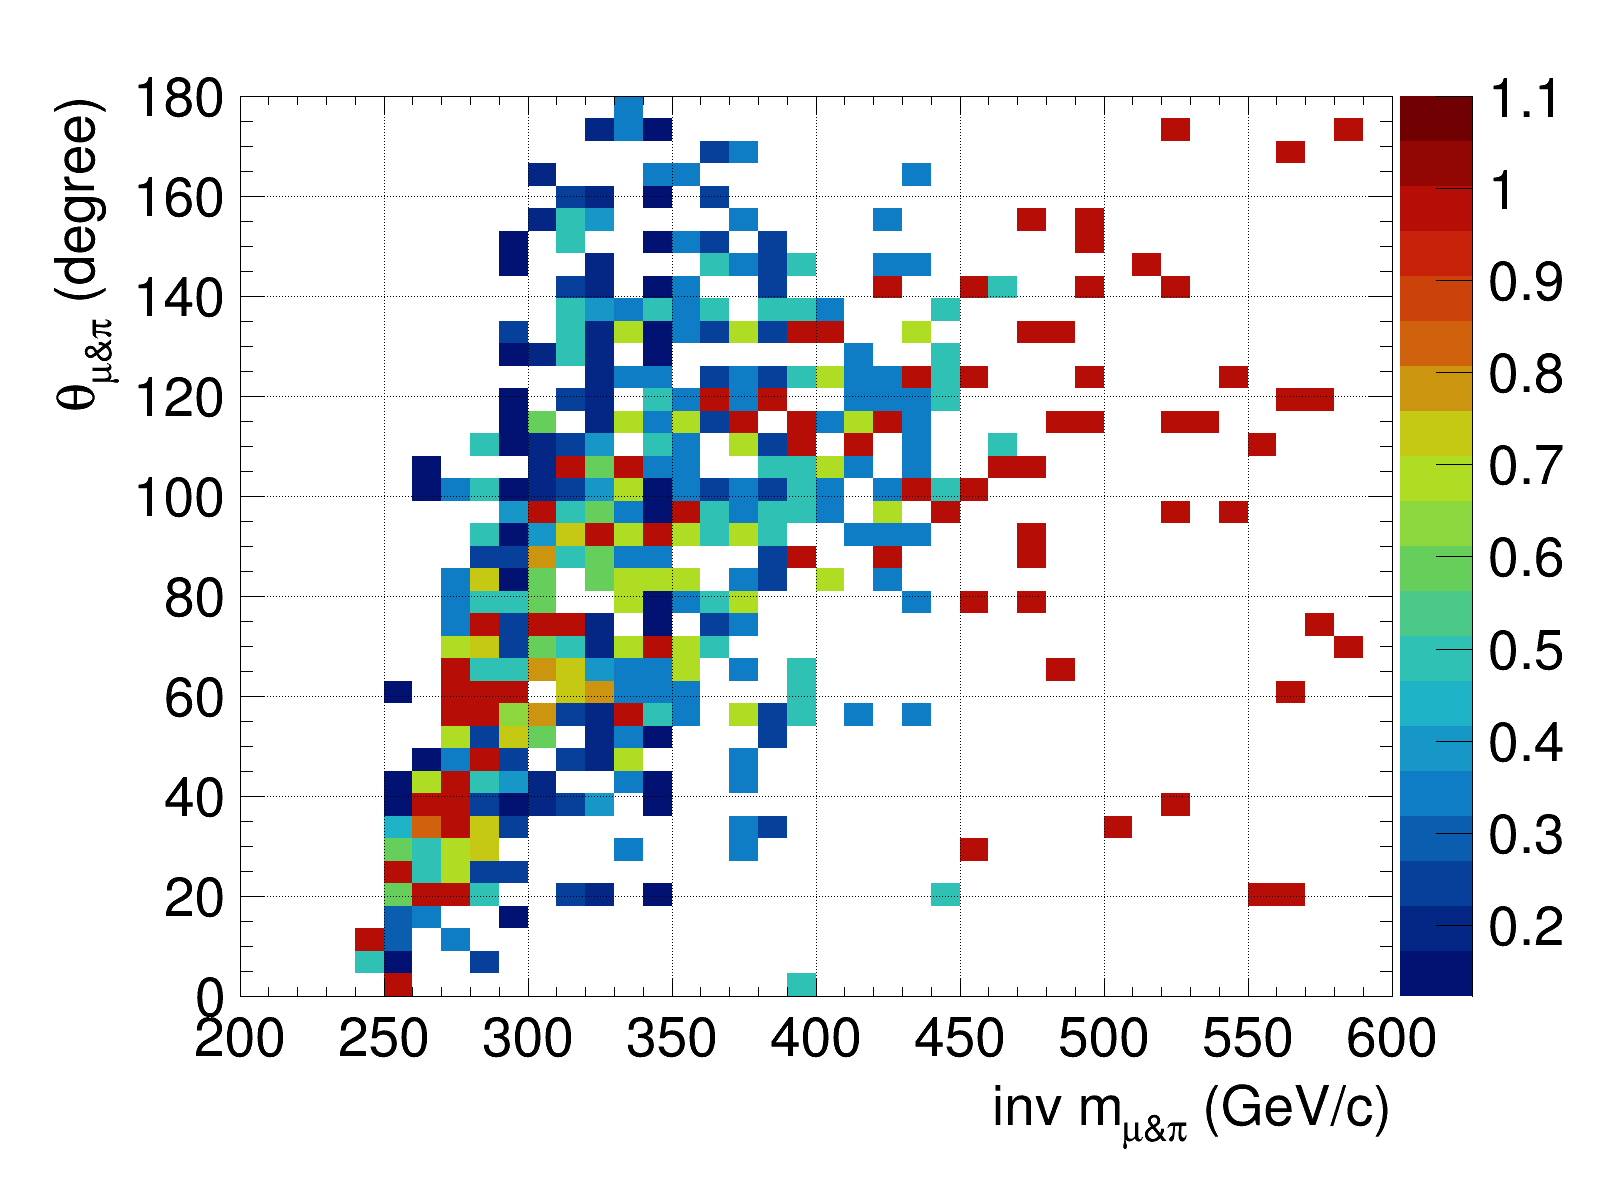
\includegraphics[width=\textwidth]{figures/hnl_sfgmu_mpinvm_colnor_vs_mpang_hist2d_al9_SM.png}
                \caption{SM $\nu$.}
                \label{fig:sm-mmupi}
           \end{subfigure}
           \caption{$\tmupi$ plotted against $\mmupi$.}
           \label{fig:mmupi-mupiang}
        \end{figure}

        \textbf{$\mu$-$\pi$ $\dpt$ cut} - Similar to the previous kinematic cuts, the net transverse momentum of $\mu$ and $\pi$ should be small while that for the SM event would have a much larger range as shown in Fig.~\ref{fig:mmupi-dpt}. By placing the cut, $\dptmupi<15~\mevc$, $8$ HNL events survived with $0$ SM backgrounds.
        
        \begin{figure}[!htb]
           \centering
           \begin{subfigure}{0.45\textwidth}
                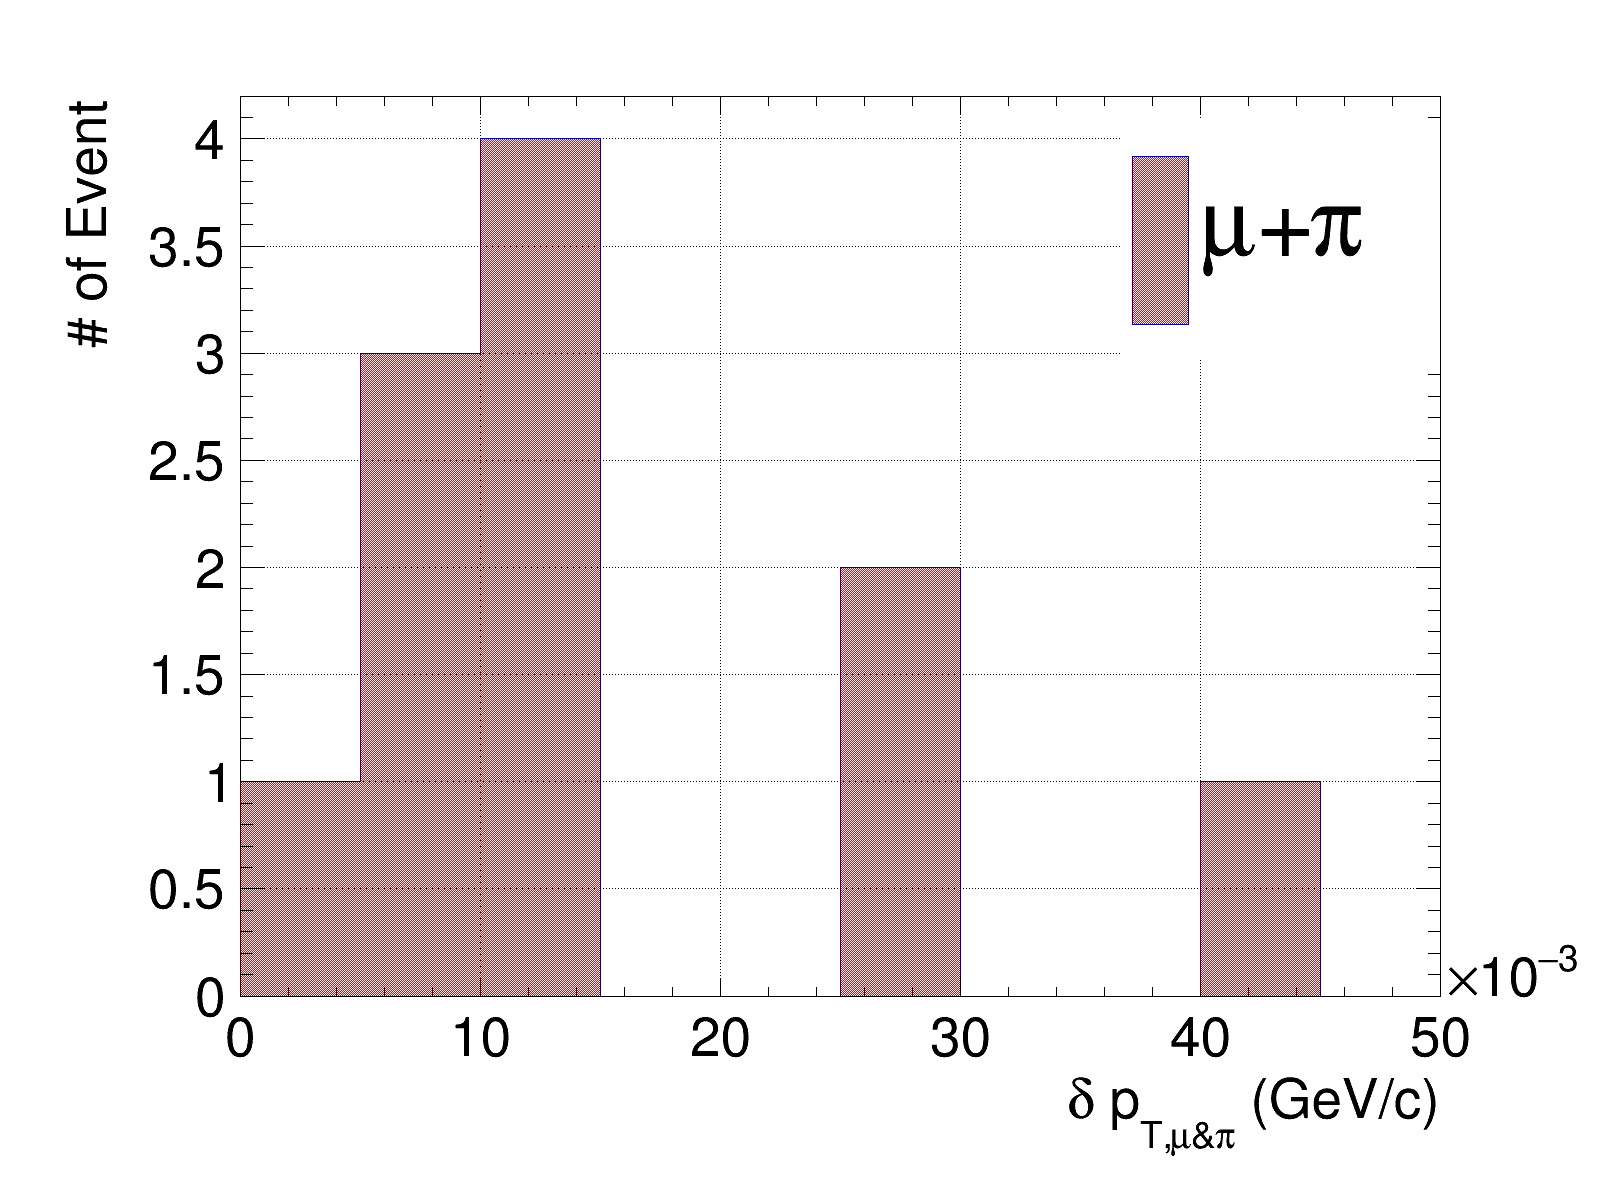
\includegraphics[width=\textwidth]{figures/hnl_sfgmu_mpdpt_stack_al9_300_aftmupikin.png}
                \caption{HNL.}
                \label{fig:hnl-mupidpt}
           \end{subfigure}
           \begin{subfigure}{0.45\textwidth}
                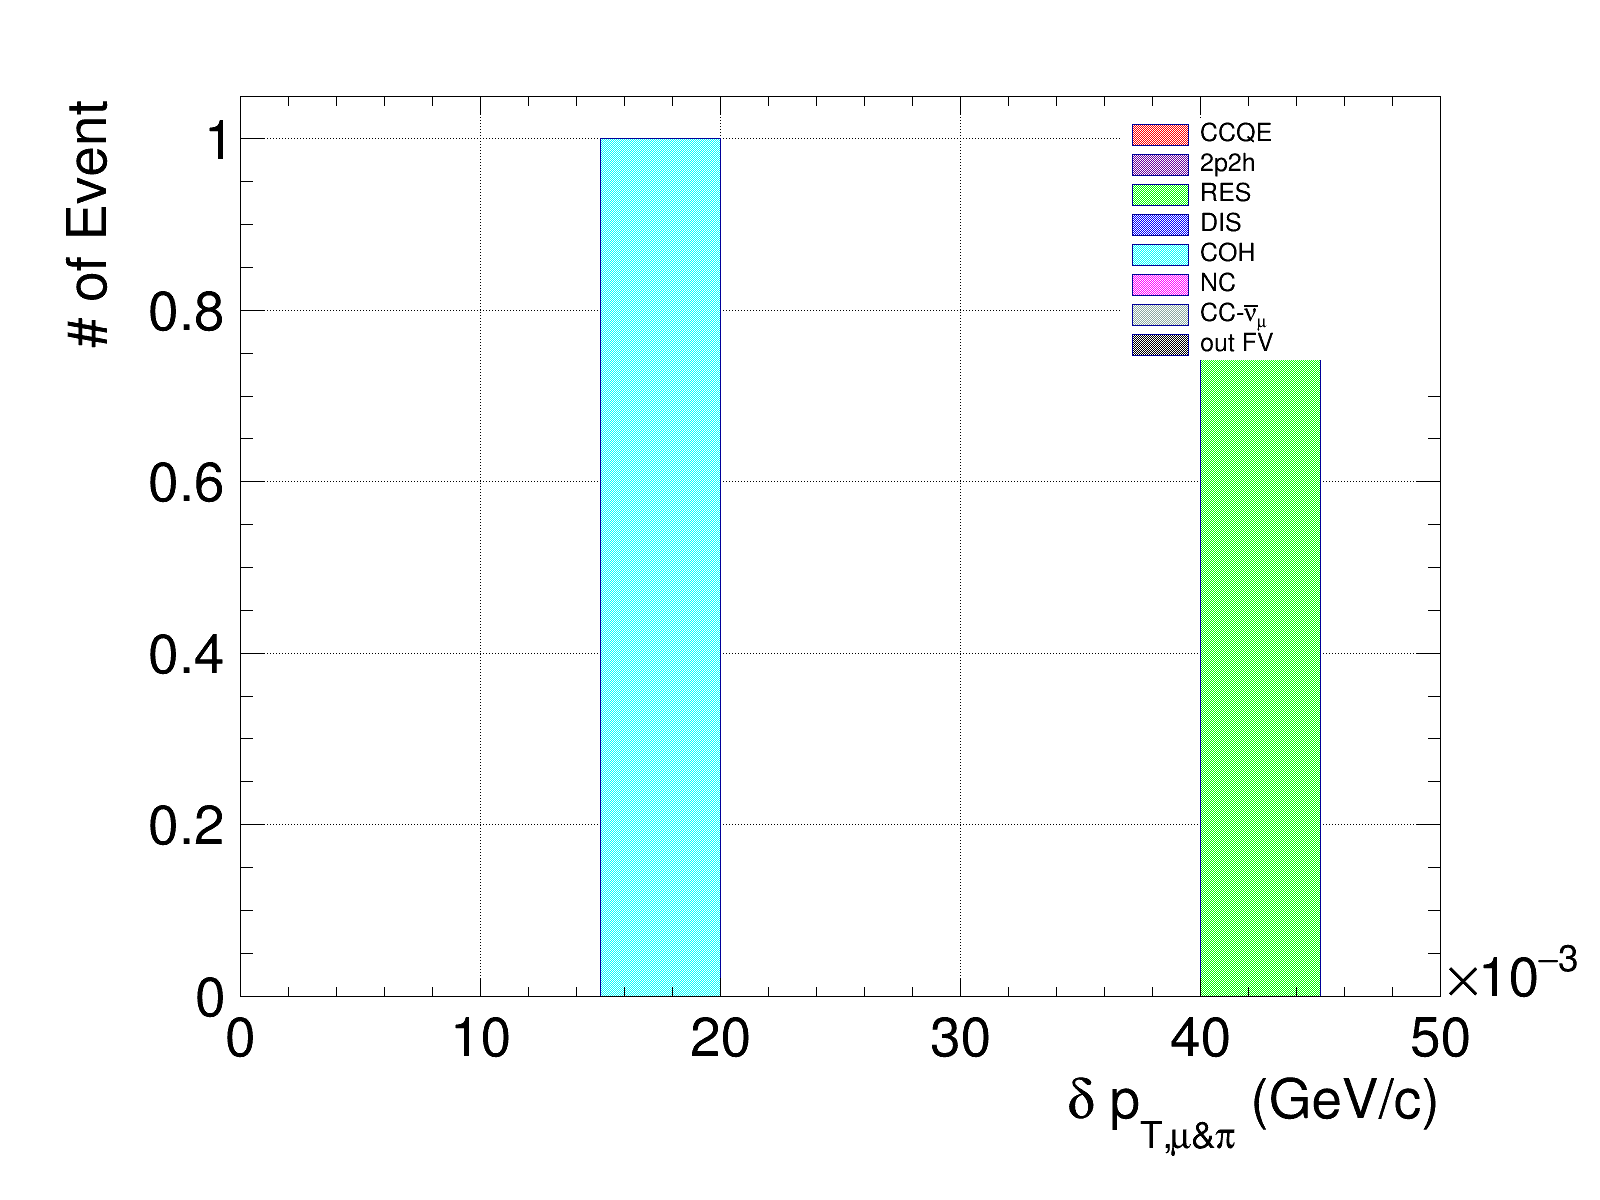
\includegraphics[width=\textwidth]{figures/hnl_sfgmu_mpdpt_stack_al9_SM_aftmupikin.png}
                \caption{SM $\nu$.}
                \label{fig:sm-mupidpt}
           \end{subfigure}
           \caption{$\dptmupi$ distributions for HNL and SM $\nv$.}
           \label{fig:mmupi-dpt}
        \end{figure}

    
    \subsubsection{Background estimation}
        A comprehensive background estimation is not finished yet, but it is suggesting, from Fig.~\ref{fig:sm-mupidpt}, and expected that coherent pion production is the dominant source. 
        From a crude estimation, as shown in Fig.~\ref{fig:coh-bkg}, the area under the fitted curve for $\dptmupi<15~\mevc$ is approximately $0.5$. 
        \begin{figure}[!htb] 
            \centering
            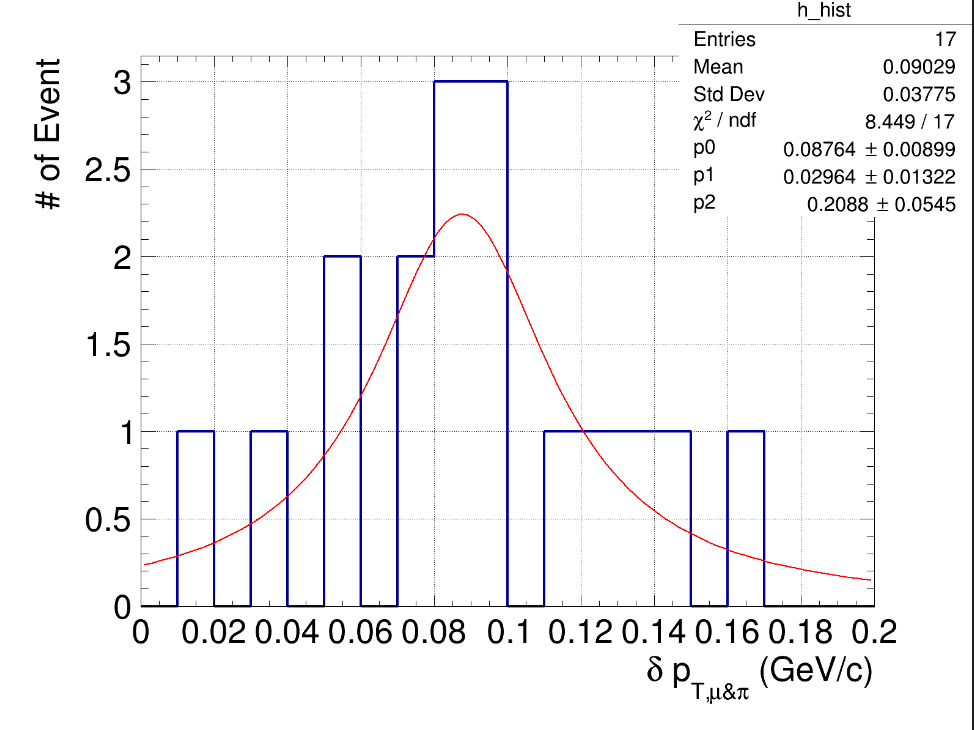
\includegraphics[width=0.5\linewidth]{figures/COH.png}
            \caption{Coherent background estimation.}
            \label{fig:coh-bkg}
        \end{figure}    
        
    \subsubsection{Sensitivity extraction}
        Sensitivity is extracted using the $CL_s$ method~\cite{Read_2002}.
        $CL_x$ is defined as $\textrm{Prob}(N\leq N_{\textrm{obs}}| \mu = x)$, i.e. the probability of predicting a number of events smaller or equal to the number of observed events assuming model $x$. When $x=b$ or $x=s+b$, it is the background-only model or the the signal plus background model.
        Then, $CL_s$ is defined as 
        \begin{equation}
            CL_s = \frac{CL_{s+b}}{CL_{b}} = \frac{\textrm{Prob}(N\leq N_{\textrm{obs}}| \mu = s+b)}{\textrm{Prob}(N\leq N_{\textrm{obs}}| \mu = b)} = \alpha,
        \end{equation}
        where $1-\alpha$ is the confidence level.

        For a target confidence level, $f$, one starts from $s=0$ and iterate with increasing $s$ to find the largest $s_{up}$ such that $\alpha < 1-f$. 
        Then $s_{up}$ is the upper limit for the number of signal events at confidence level $f$ such that the background-only model is not rejected. 
        When a more detailed background model is available, it is conventional to pick the median number of background events to evaluate $s_{up}$.
        A limit can then be placed on the mixing element $\umas$ from its proportional relation to $s_{up}$.

        Specifically in the above example, $100,000$ \genie events were simulated using \code{BeamHNL}. 
        The total number of protons on target (POT) required to produce these HNL events are calculated from \code{BeamHNL} output to be approximately $0.81\times10^{21}$ assuming $\umas=10^{-7}$. 
        Hence, we expect $8/0.81\approx9.9$ selected signals per $10^{21}$ POT.
        For this estimation, background is taken to be $0.5$, then $s_{up}$ is calculated to be $2.3$. 
        Hence, the limit on $\umas$ is calculated as 
        \begin{align}
            (\frac{U_{up}}{10^{-7}})^2 & =  2.3 / 9.9 \\
            U_{up} & = 10^{-7} \times \sqrt{2.3/89} = 4.8\times10^{-8}
        \end{align}

        \subsubsection{Discussion}
        This result is larger than the limit placed by the previous search, $U_{up}\approx4\times10^{-9}$, for $\mn=300~\mev$. 
        However, it is roughly of the same order of magnitude. 
        Moreover, the current result includes only events in SFGD, which is only about $1/3$ in volume compared to the vertical TPCs. 
        Most importantly, this preliminary result demonstrates that SFGD can also provide excellent signal-background separation for HNL searches.
        Hence, it will definitely improve the limits by adding it to the existing search. 
        Next step is to extend the selection to the whole upgraded ND280 when the HAT reconstruction becomes available and investigate the overall improvement in HNL sensitivity brought by the upgrade. 
 
\begin{savequote}[8cm]
\textlatin{Neque porro quisquam est qui dolorem ipsum quia dolor sit amet, consectetur, adipisci velit...}

There is no one who loves pain itself, who seeks after it and wants to have it, simply because it is pain...
  \qauthor{--- Cicero's \textit{de Finibus Bonorum et Malorum}}
\end{savequote}

\chapter{\label{ch:7-com}Centre-of-momentum variables} 

\section{Introduction}
Significant efforts have been devoted to measuring Charge-Parity (CP) violation in the neutrino sector through long-baseline (LBL) experiments. 
\blue{In these experiments, CP violation is quantified by the difference between neutrino oscillation and anti-neutrino oscillation. 
LBL experiments quantify $\dcp$ by comparing the energy spectra of $\nue$ and $\nuebar$ oscillated from $\numu$ and $\numubar$, respectively.
There are two major challenges to this measurement. 
Firstly, the far detector of an LBL experiment is by design hundreds of kilometres away from the neutrino source, which unavoidably lead to low statistics.
Secondly, as the energy of each incoming neutrino is unknown and thus the type of the individual neutrino bound-nucleon interaction is also unknown, oscillation predictions have to take the form of energy spectra for a chosen final state topologies.
Accurate $\dcp$ measurements heavily depend on neutrino interaction models estimating contributions of different neutrino-nucleon interactions to final-state topologies~\cite{NuSTEC:2017hzk}.
Large-scale experiments, such as Hyper-Kamiokande~\cite{Hyper-Kamiokande:2018ofw} and the Deep Underground Neutrino Experiment (DUNE)~\cite{DUNE:2015lol,DUNE:2016evb,DUNE:2016hlj,DUNE:2016rla,DUNE:2021tad}, address this challenge by constructing gigantic far detectors to increase event rates.
To match the reduction of statistical uncertainties, it is critical to develop advanced neutrino interaction models or to better constrain existing ones to minimize the systematic uncertainties.}

To better understand the complex neutrino-nucleus interactions, new or upgraded experiments with sophisticated detectors have commenced to explore a larger interaction kinematic phase space and to collect a significantly larger amount of data. 
For instance, the Tokai-to-Kamioka (T2K) experiment~\cite{T2K:2011qtm} has upgraded its near detector (ND) and started data collection in June 2024. 
The Super Fine-Grain Detector (SFGD), part of the T2K ND upgrade~\cite{T2K:2019bbb}, provides improved proton detection with lower thresholds, higher resolution, and greater efficiency. 
Meanwhile, the Short-baseline Near Detector (SBND)~\cite{MicroBooNE:2015bmn} has also begun operations in 2024. 
It is a new LArTPC with an active mass of 112 ton placed at $110$ m from the neutrino source. 
Due to its large active mass and proximity to the source,  it is expected to collect a huge number of neutrino interaction events each year.  
On one hand, the expanded kinematic phase space allows for measuring new variables. 
On the other, the influx of high-quality data offers an ideal testing ground for novel measurement techniques.
Taking advantage of these advancements, it is timely to explore new ideas involving pions in the final states, given the broad energy spectrum of the DUNE beamline, which includes substantial contributions from resonance production comparable to quasi-elastic interactions, 

One effective method of utilizing the near detector data is to constrain model parameters through tuning.
Successful examples~\cite{GENIE:2021zuu,GENIE:2021wox,GENIE:2022qrc} have shown improved data-Monte Carlo (MC) agreement after tuning existing models using various combinations of measurements from different experiments. 
However, the neutrino-nucleus interaction is a convolution of multiple processes: the nucleon initial state (IS), the neutrino-nucleon interaction, and final state interactions (FSI). 
Many variables are affected by all these processes, making it challenging to study the different models in isolation. 
Nuclear effects, such as IS and FSI, occur within the nucleus and remain unobservable with current detectors, making them a major source of systematic uncertainties.
Cleverly constructed variables, such as Transverse Kinematic Imbalance (TKI)~\cite{Lu:2015hea, Lu:2015tcr} or Generalized Kinematic Imbalance (GKI)~\cite{MicroBooNE:2023krv}, are sensitive to nuclear effects, and past measurements have successfully constrained models~\cite{GENIE:2024ufm}. 
While TKI is sensitive to both IS and FSI, except $\dat$, which is predominantly sensitive to FSI but is affected by small uncertainties in the neutrino direction, new variables like $\plong$ \cite{Baudis:2023tma} are designed to be sensitive to specific nuclear effects, such as the removal energy. 

Having more specialized measurements, like $\plong$, can further fine-tune our models, especially in light of the improved detection capabilities. 
This work proposes a new set of variables, called center-of-momentum (COM) variables, for charge current single pion single proton ($\ccopiop$) events, timely for the increasingly precise measurements with pions in the final states
COM variables enable more focused studies of FSI by differentiating between FSI models independently of IS models.

This paper will elaborate on the concept of the COM variables and present MC analysis results focusing on the COM angle and demonstrating its ability to distinguish FSI models and its independence from IS.

\section{The COM Variables}



\minitoc
\begin{savequote}[8cm]
Everything comes to him who knows how to wait.

  \qauthor{--- Wolfgang Pauli }
\end{savequote}

\chapter{\label{ch:concl}Epilogue} 

\minitoc

Back in October 2022, I traveled to Tokai to join the task force responsible for assembling the SFGD.
We began by constructing the outer box to hold the cubes together, and the first layer was installed on October 28th.
For approximately two months, we meticulously stacked the scintillator cubes layer by layer, aligning each new layer with great effort.
As the number of layers increased, maintaining vertical alignment became progressively more challenging due to the growing friction between the accumulating cubes.
Initially, vertical alignment was achieved using thin metal rods approximately 10 cm in length, which soon proved too short.
The original plan was to utilize fishing lines for subsequent alignments; however, it quickly became evident that they lacked the necessary strength to shift the cubes in alignment.
Fortunately, we were able to purchase longer metal rods in time, preventing the need to undertake an impossible task.
The final layer was added in December just before the new year.

After a short break, we proceeded to the next task: fiber insertion.
With more team members joining, the workforce became sufficiently large and the workflow sufficiently independent to allow for a clear division of labor.
Some team members were responsible for removing the fishing lines that held the cubes together during layer installation, others pushed the optical fibers through the designated holes where the fishing lines had been removed, and some maintained a constant supply of fibers for the fiber pushers.
The fiber insertion process took an additional two months.
Afterward, I returned to focus on my analysis work while the electronics were diligently added and calibrated.
The assembly was finally completed in October 2023 and was ready to be installed in the ND280 pit.
In June 2024, the entire ND280 upgrade was completed and began taking data for the first time.
The data event display images presented in this thesis were collected during the June 2024 run.

As a doctoral student, assembling a detector and witnessing its functionality was a truly unique and fortunate experience.
Although it is unfortunate that there was not enough time to perform a full cross-section measurement using the new data, my Monte Carlo (MC) analysis and the preliminary data-MC comparisons demonstrate the far-reaching physics potential of the upgraded ND280.
The upgraded detector will be capable of measuring the TKI and COM variables with unprecedented precision.
My tuning project, utilizing existing TKI measurements, already shows promising improvements in neutrino interaction modeling.
It is thus exciting to anticipate the advancements in interaction modeling that future TKI and COM measurements of ND280 will bring.
Beyond advancing SM physics, my HNL sensitivity study of the SFGD demonstrates that it possesses comparable HNL detection capabilities to the gaseous TPCs.
Consequently, the entire upgraded ND280 boasts a detection volume nearly twice its previous size.
Combined with the forthcoming beamline upgrade, T2K has the potential to conduct the most sensitive searches for HNLs produced from kaon and pion decays.

New and upgraded experiments, such as JUNO and SBND, around the world have either commenced operations or are about to do so.
Hyper-K and DUNE are also under active construction.
It is optimistic that we will achieve a sufficient understanding of neutrino interactions, enabling next-generation LBL experiments to make precise measurements of $\delta_{\text{CP}}$ within our lifetime.
I hope that my work can contribute to shortening this timeline, even if only slightly, and when that day arrives, I will be gratified.
\begin{savequote}[8cm]
\textlatin{Neque porro quisquam est qui dolorem ipsum quia dolor sit amet, consectetur, adipisci velit...}

There is no one who loves pain itself, who seeks after it and wants to have it, simply because it is pain...
  \qauthor{--- Cicero's \textit{de Finibus Bonorum et Malorum}}
\end{savequote}

\chapter{\label{ch:5-tki}TKI} 

\minitoc

\section{\label{sec:1-intro}Introduction}

Neutrinos play a central role in advancing our understanding of physics and addressing fundamental inquiries in contemporary science. The Hyper-Kamiokande experiment~\cite{Hyper-Kamiokande:2018ofw} aims to conduct precise measurements of charge parity violation within the neutrino sector, a phenomenon believed to be closely linked to the observed matter-antimatter asymmetry in the universe. Similarly, the Deep Underground Neutrino Experiment (DUNE)~\cite{DUNE:2016hlj,DUNE:2015lol,DUNE:2016evb,DUNE:2016rla,DUNE:2021tad}  promises the same, in addition to elucidating the neutrino mass ordering. Whether seeking to ascertain Standard Model parameters or probing for exotic phenomena, significant enhancements in both theoretical frameworks and computational simulations of neutrino-nucleus interactions are imperative. As neutrinos interact mainly with nucleons inside the nucleus, the interaction is subject to nuclear effects, namely the nucleon initial state and final-state interactions (FSIs). These effects are difficult to calculate and can alter the final event topology by changing the number of final state pions with respect to the interactions on free nucleons. Notably, the neutrino flux at DUNE yields a comparable proportion of events with and without pions in the final state, highlighting the pressing need for a generator capable of accurately describing both event topologies.

The large data samples and superb imaging capabilities of modern neutrino experiments offer us a detailed new look at neutrino interaction physics.
Recently, the GENIE~\cite{Andreopoulos:2009rq, GENIE:2021npt} Collaboration has made substantial progress towards a global tuning using neutrino, charged lepton and hadron scattering data, in an attempt to integrate new experimental constraints with state-of-the-art theories and construct robust and comprehensive simulations of neutrino interactions with matter. 
Cross-experiment and cross-topology analyses are challenging tasks as each measurement features its unique selection criteria and various other  aspects, such as the neutrino flux. \genie has built an advanced tuning framework that enables the validation and tuning of comprehensive interaction models using an extensive curated database of measurements of neutrino, charged lepton and hadron scattering off nucleus and nuclei. So far, the non-resonant backgrounds~\cite{GENIE:2021zuu}, hadronization~\cite{GENIE:2021wox} and the quasielastic (QE) and 2-particle-2-hole (2p2h)  components~\cite{GENIE:2022qrc} of the neutrino-nucleus interaction have been tuned with $\nu_\mu$ and $\bar{\nu}_\mu$ charged-current (CC) pionless (0$\pi$) data from MiniBooNE, T2K and MINERvA. A partial tune was performed for each experiment, highlighting the neutrino energy dependence on the QE and 2p2h tuned cross sections. Even though post-tune predictions enhanced the data description for each experiment, the added degrees of freedom were not sufficient to fully describe all CC0$\pi$ data and exhibited tensions with some proton observables~\cite{GENIE:2022qrc}. More exclusive measurements result in additional model constraints. In addition, observables that are sensitive to targeted aspects of the complex dynamics of neutrino interactions are invaluable for model tuning. The transverse kinematic imbalance (TKI)~\cite{Lu:2015hea, Lu:2015tcr}, a final-state correlation between the CC lepton and the handronic system, is a good example since it is sensitive to the initial-state nuclear environment and hadronic FSI. Our next step is to incorporate TKI data from experiments where various exclusive topologies at different energies are considered. This marks the first combined tuning on TKI data with and without pions in the final states and serves as the starting point of a more comprehensive tuning effort in the energy region most relevant for future accelerator-based neutrino experiments.  

This paper is structured as follows: In Sec.~\ref{sec:tki} and Sec.~\ref{sec:genie}, we review the TKI measurements and \genie models respectively. In Sec.~\ref{sec:Tuning}, we detail the tuning considerations and procedures. Results are summarized in Sec.~\ref{sec:results}, highlighting how the data-MC discrepancy in the \minpiz TKI measurement~\cite{MINERvA:2020anu} is resolved while maintaining good data-MC agreement elsewhere. We conclude in Sec.~\ref{sec:summary}. 

\section{TKI measurements}\label{sec:tki}


TKI is a methodology based on the conservation of momentum in neutrino interactions. In essence, it involves quantifying the imbalance between the observed transverse momentum of the final-state particles and the expected transverse momentum from neutrino interactions with free nucleons~\cite{Lu:2015hea, Lu:2015tcr}. This ``kinematic mismatch'' together with its longitudinal and three-dimensional variations~\cite{Furmanski:2016wqo, Lu:2019nmf}, and the derived asymmetry~\cite{Cai:2019jzk}, has been a crucial set of observables, establishing a pathway to extract valuable information about the participating particles and the underlying nuclear processes. Recent experimental results from neutrino experiments such as  T2K~\cite{T2K:2018rnz, T2K:2021naz}, MINERvA~\cite{MINERvA:2018hba, MINERvA:2019ope, MINERvA:2020anu, MINERvA:2021csy}, and MicroBooNE~\cite{MicroBooNE:2022emb, MicroBooNE:2023cmw, MicroBooNE:2023tzj, MicroBooNE:2023wzy, MicroBooNE:2024tmp}, as well as electron scattering experiments such as  CLAS~\cite{CLAS:2021neh}, highlight the efficacy of TKI. 

\begin{figure}[!htb] 	
    \centering 		
    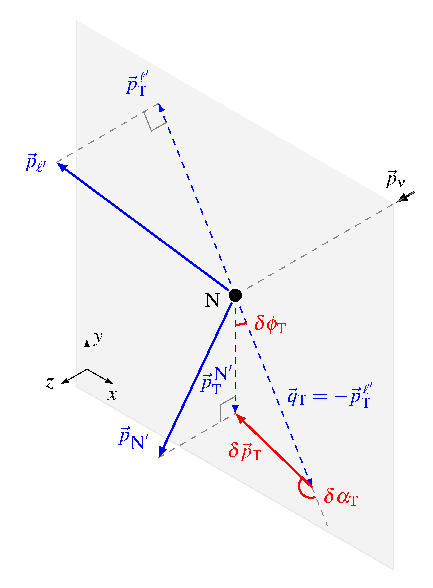
\includegraphics[width=0.35\textwidth]{figures/stki.eps}
    \caption{\label{fig:stki} Schematic illustration of the TKI variables. Diagram taken from Ref.~\cite{Lu:2015tcr}.} 
\end{figure}

In neutrino scattering off a free nucleon, the sum of the transverse components of the final products is expected to be zero, visualized through a back-to-back configuration between the final-state lepton and hadronic system in the  plane transverse to the neutrino direction. Hence, in a neutrino interaction with a nucleus, the transverse momentum imbalance, $\dpt$~\cite{Lu:2015tcr}, results from intranuclear dynamics, including Fermi motion and FSIs  as shown in Fig.~\ref{fig:stki}. The deviation from being back-to-back is quantified by the  coplanarity angle $\dphit$~\cite{Lu:2015tcr}, while the transverse boosting angle, $\dat$~\cite{Lu:2015tcr}, represents the direction of $\dpt$ within the transverse plane. Furthermore, analyzing the energy and longitudinal momentum budget~\cite{Furmanski:2016wqo, Lu:2019nmf} enables the conversion of $\dpt$ to the emulated (initial) nucleon momentum, $\pn$,  providing further insight into the Fermi motion; this conversion amounts to a correction on the order of $\mathcal{O}(20\%)$~\cite{Yang:2023dxk}. 
With one-body currents in the absence of FSIs, $\dat$ remains uniform (except for second-order effects, such as variations in the center-of-mass energy), given the isotropic nature of the initial nucleon motion. However, as the final products propagate through the nuclear medium, they experience FSIs, thereby disturbing the isotropy and the Fermi motion peak of the $\dat$ and $\pn$ ($\dpt$) distributions, respectively. Hence, $\dpt$ and $\pn$ elucidate the Fermi motion details, while $\dat$  characterizes the FSI strength---crucial for understanding medium effects in neutrino interactions. A notable advantage of these observables is their minimal dependence on neutrino energy~\cite{Lu:2015tcr}. Moreover, the double TKI variable, $\dptt$~\cite{Lu:2015hea}, is the projection of $\vecdpt$ along the axis perpendicular to the lepton scattering plane (hence ``double''). In addition to its use for extracting neutrino-hydrogen interactions~\cite{Lu:2015hea, Hamacher-Baumann:2020ogq}, it has also been applied to study nuclear effects in neutrino pion productions~\cite{MINERvA:2020anu, T2K:2021naz}. Its equivalent in pionless production, $\dptx$, has been proposed and studied together with its orthogonal companion, $\dpty$, in MINERvA~\cite{MINERvA:2019ope}. 

This work surveyed four TKI data sets: T2K $0\pi$~\cite{T2K:2018rnz}, T2K $\pi^+$~\cite{T2K:2021naz}, MINERvA $0\pi$~\cite{MINERvA:2018hba, MINERvA:2019ope}, and MINERvA $\pi^0$~\cite{MINERvA:2020anu} measurements. All four measurements require the presence of one CC muon and at least one proton in the final state. While the \ttkpip measurement requires exactly one $\pi^+$, and \minpiz requires at least one $\pi^0$, the other two datasets require the absence of any pions. The definitions of the kinematic cuts for these samples are summarized in Table~\ref{tab:data-sets-phase-space-cut}. 

\begin{figure*} 
    \centering 		
    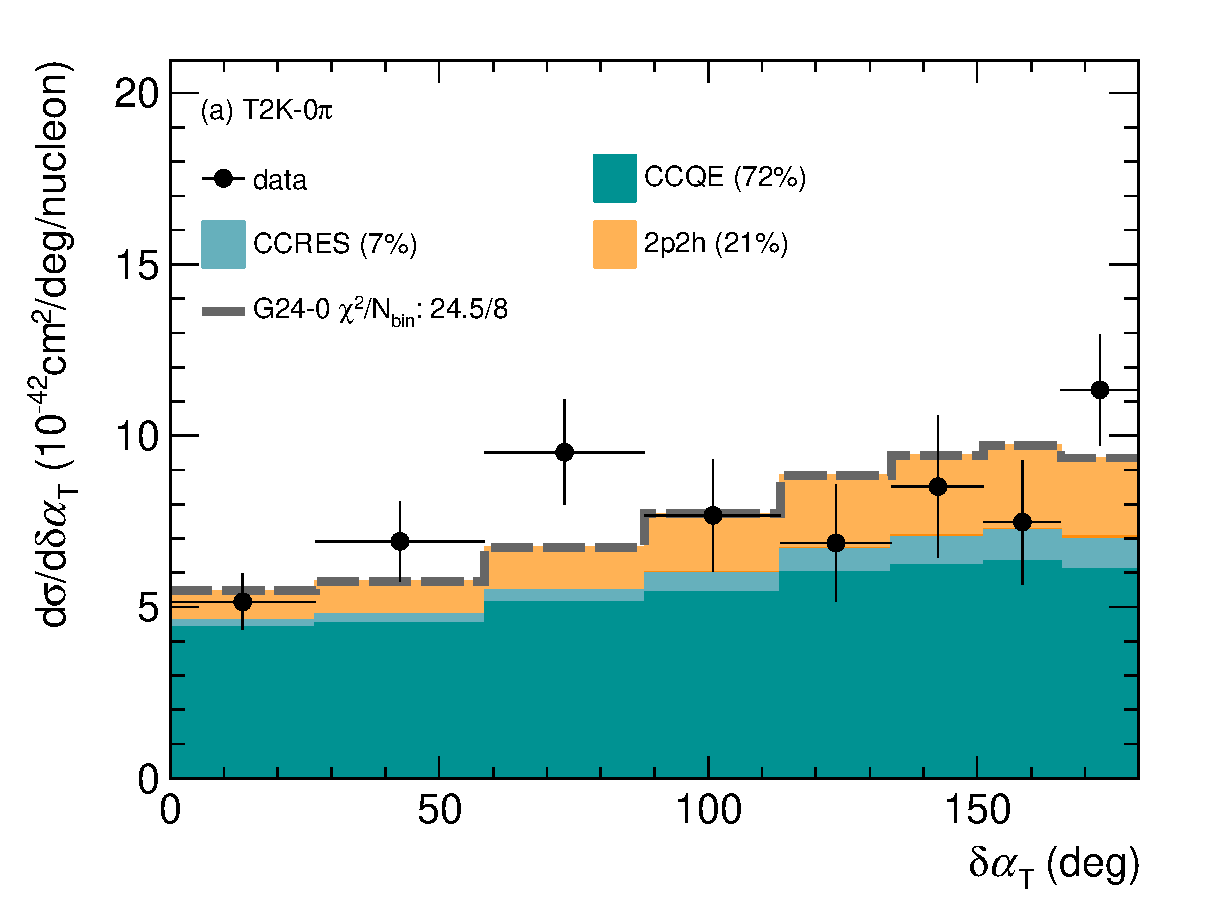
\includegraphics[width=\dbfigwid\textwidth]{figures/0000-t2k_0pi_dalphat_reac_decomp.eps} 
    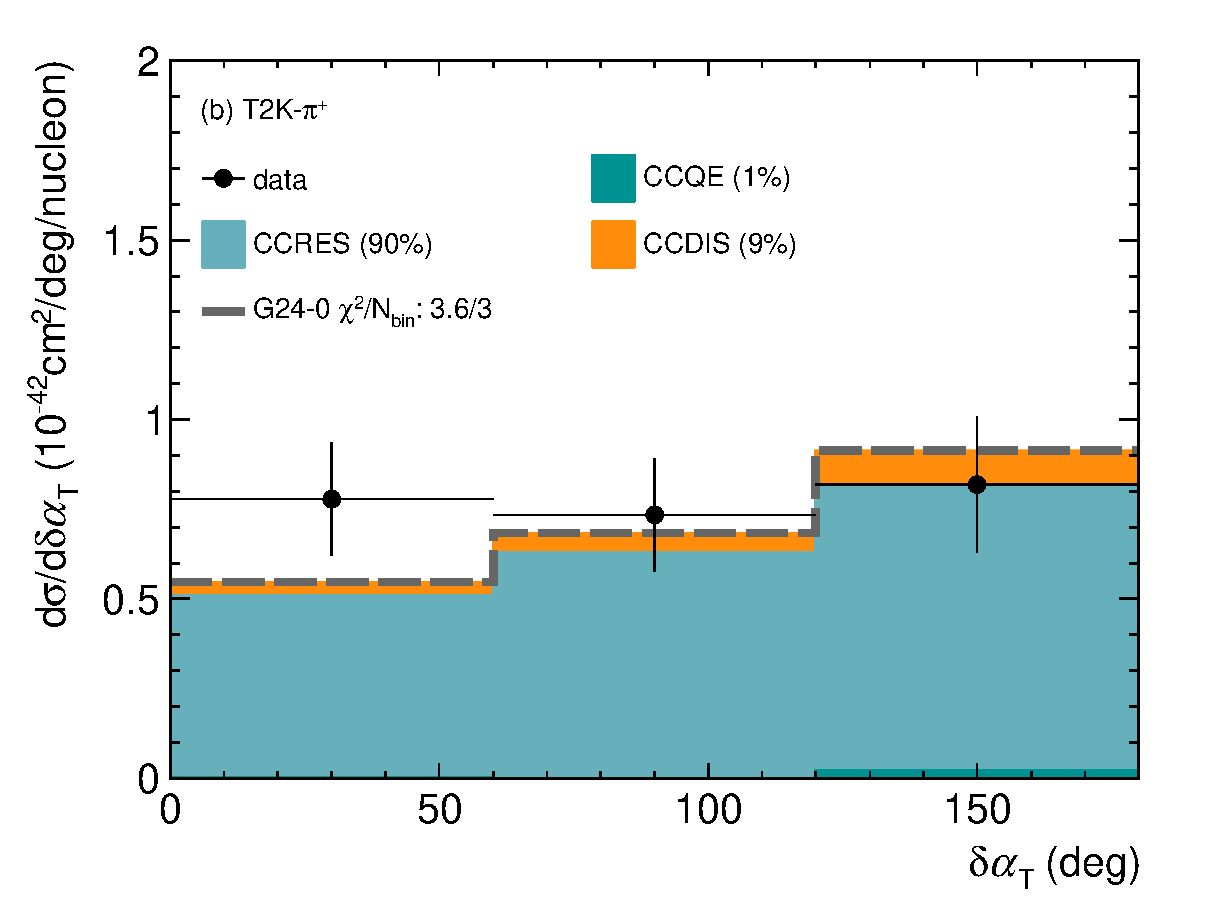
\includegraphics[width=\dbfigwid\textwidth]{figures/0000-t2k_pip_dalphat_reac_decomp.eps} 
    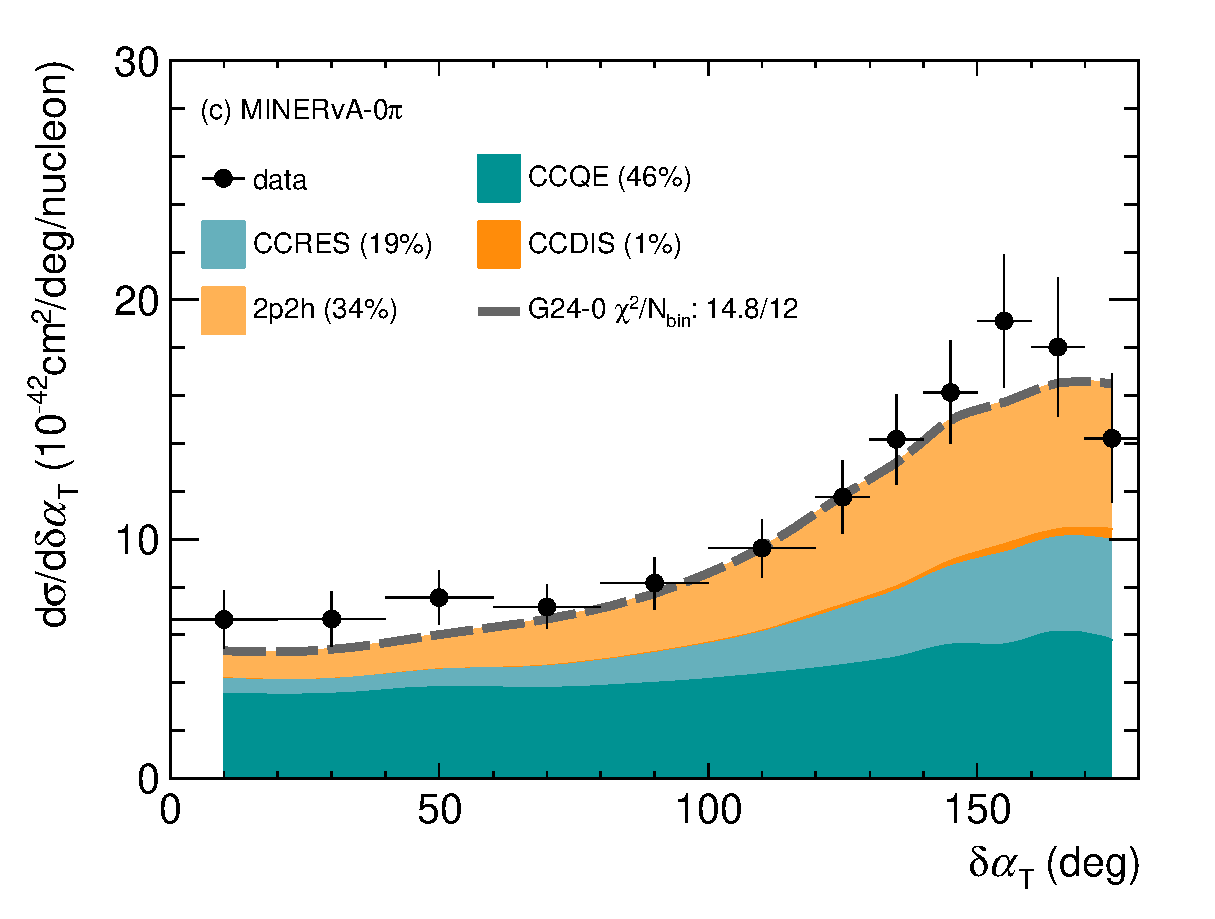
\includegraphics[width=\dbfigwid\textwidth]{figures/0000-min_0pi_dalphat_reac_decomp.eps} 
    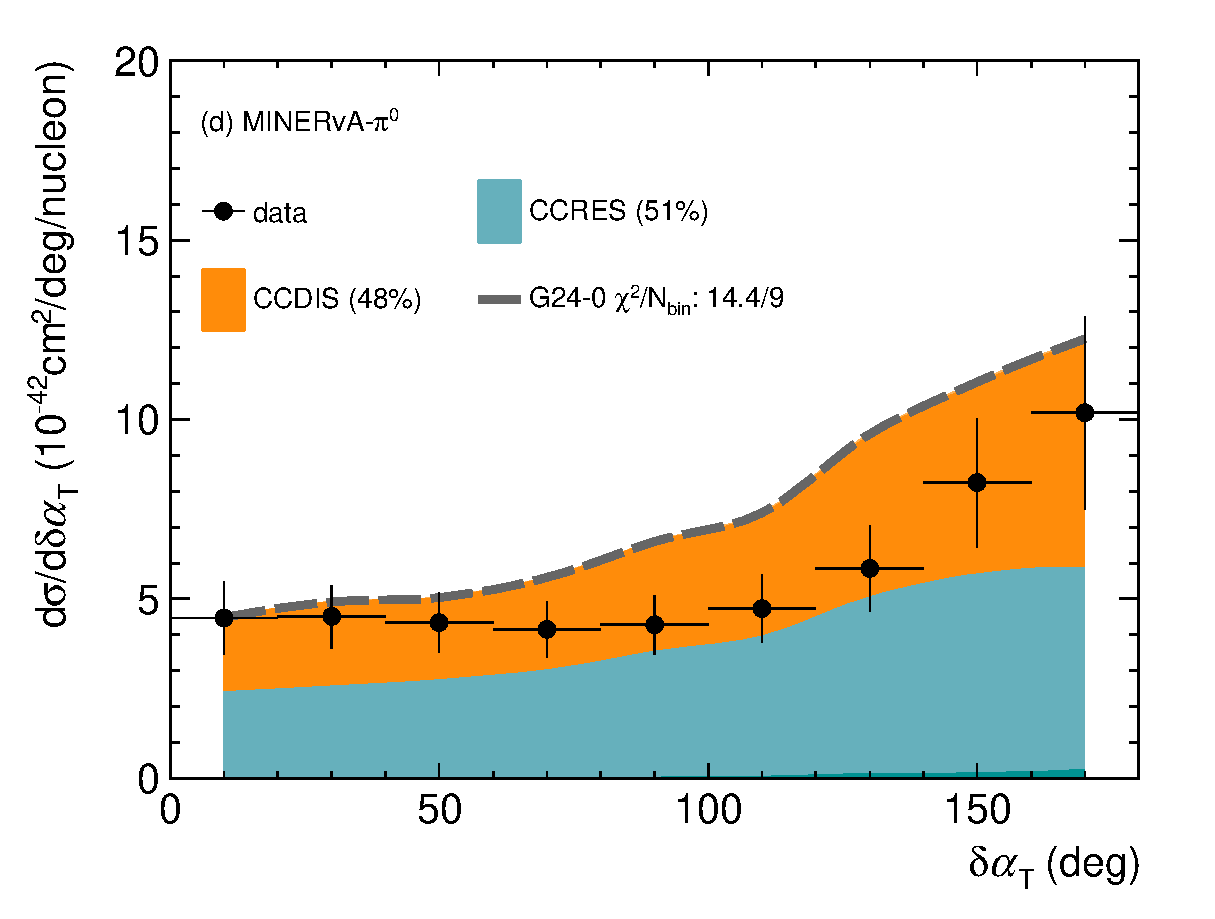
\includegraphics[width=\dbfigwid\textwidth]{figures/0000-min_pi0_dalphat_reac_decomp.eps}
    \caption{$\dat$ measurements decomposed in interaction types, compared to \gZero prediction.}   \label{fig:g24-0-dat-reac} 
    		
    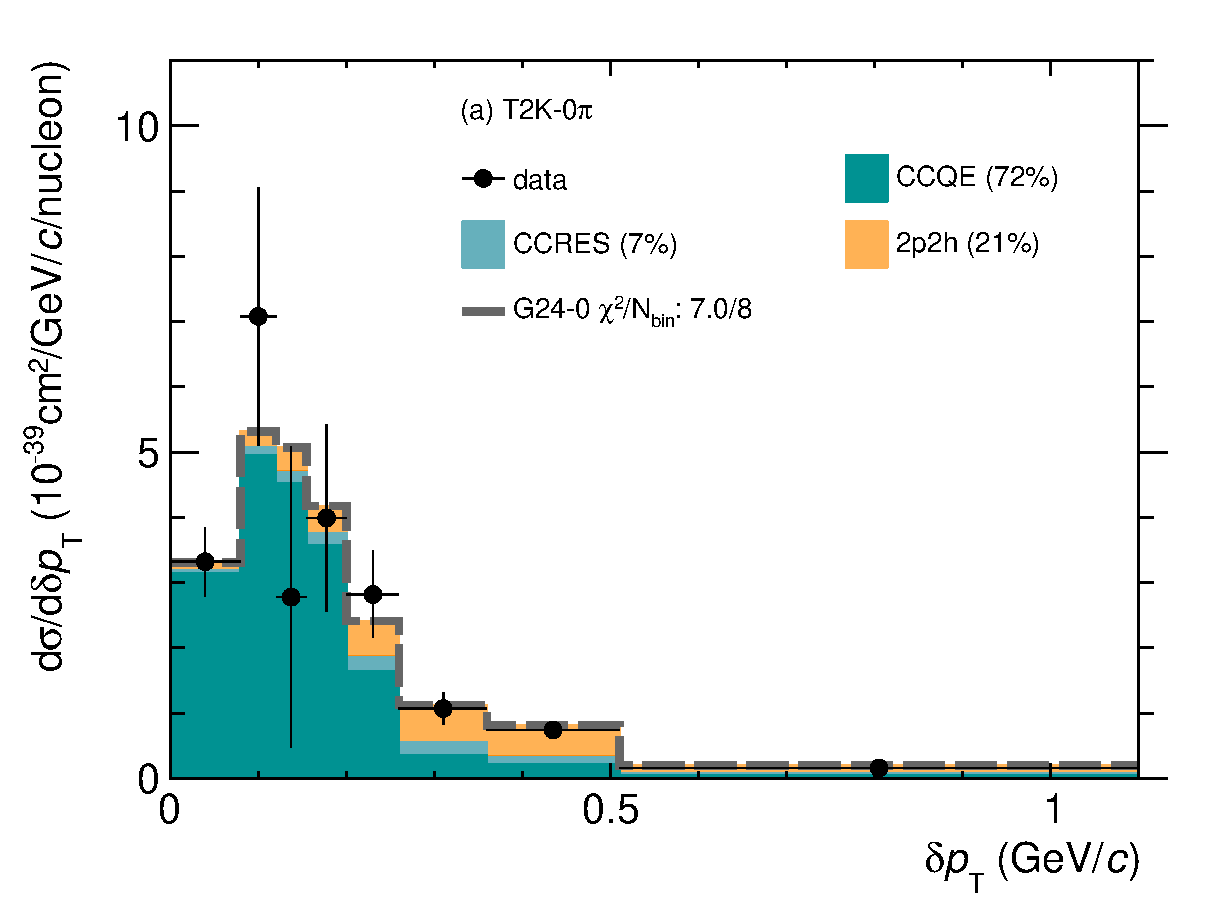
\includegraphics[width=\dbfigwid\textwidth]{figures/0000-t2k_0pi_dpt_reac_decomp.eps}
    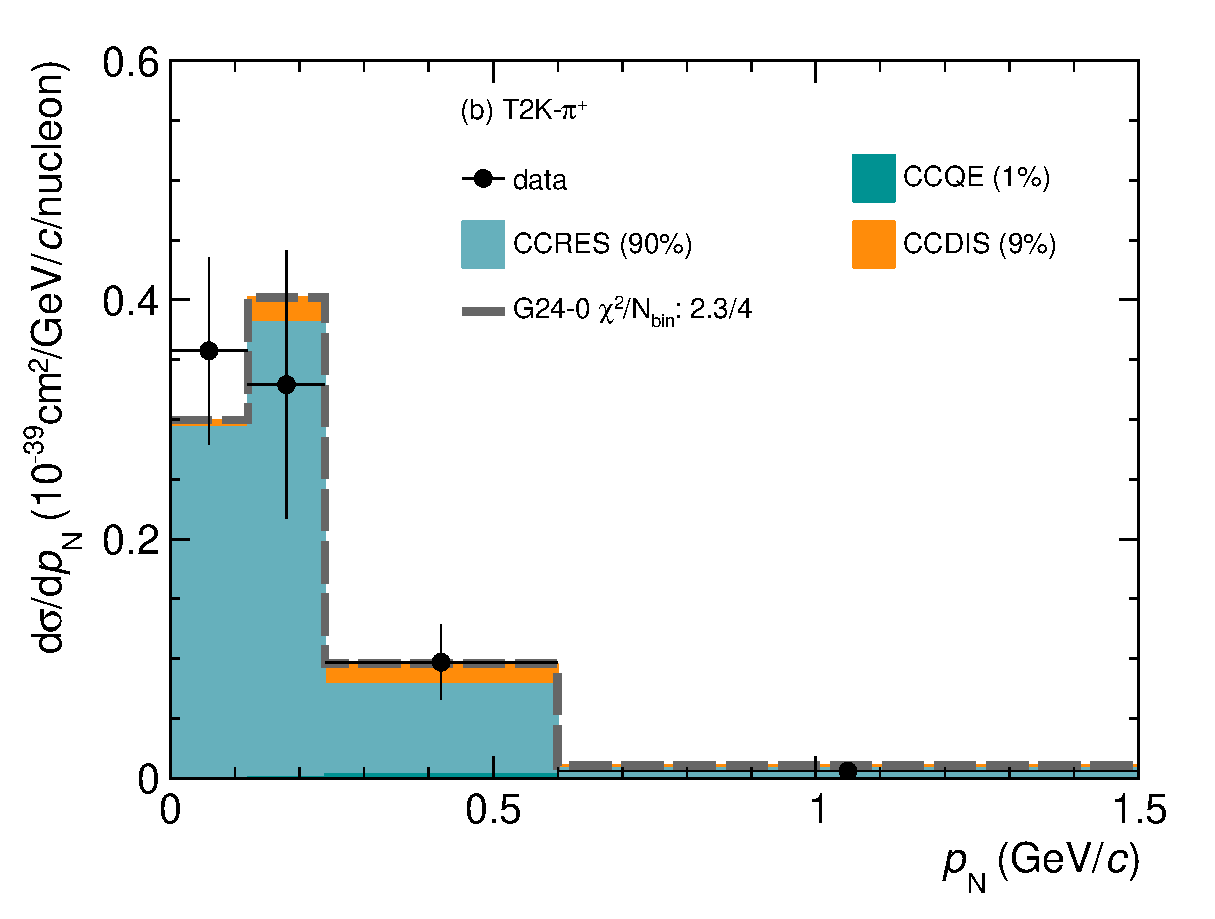
\includegraphics[width=\dbfigwid\textwidth]{figures/0000-t2k_pip_pn_reac_decomp.eps}
    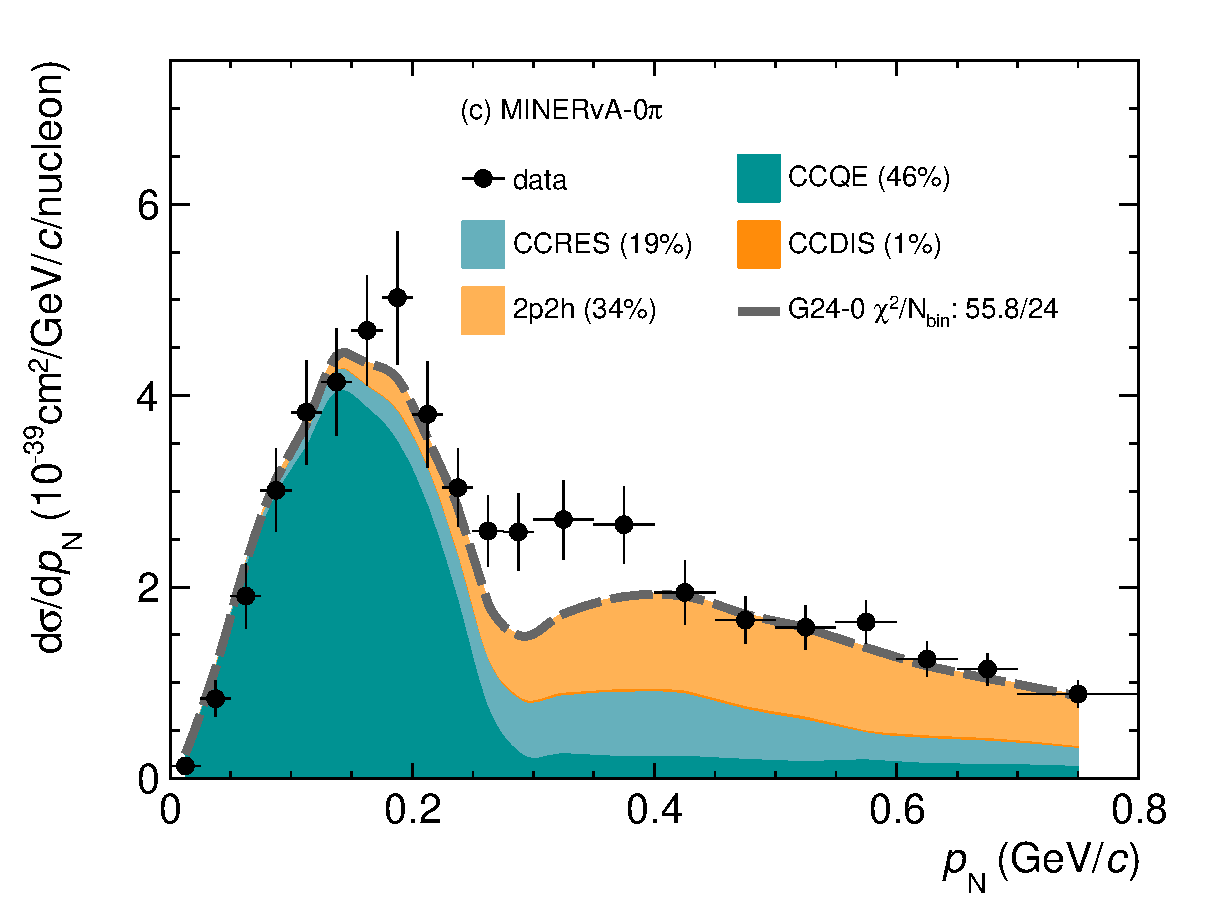
\includegraphics[width=\dbfigwid\textwidth]{figures/0000-min_0pi_pn_reac_decomp.eps}
    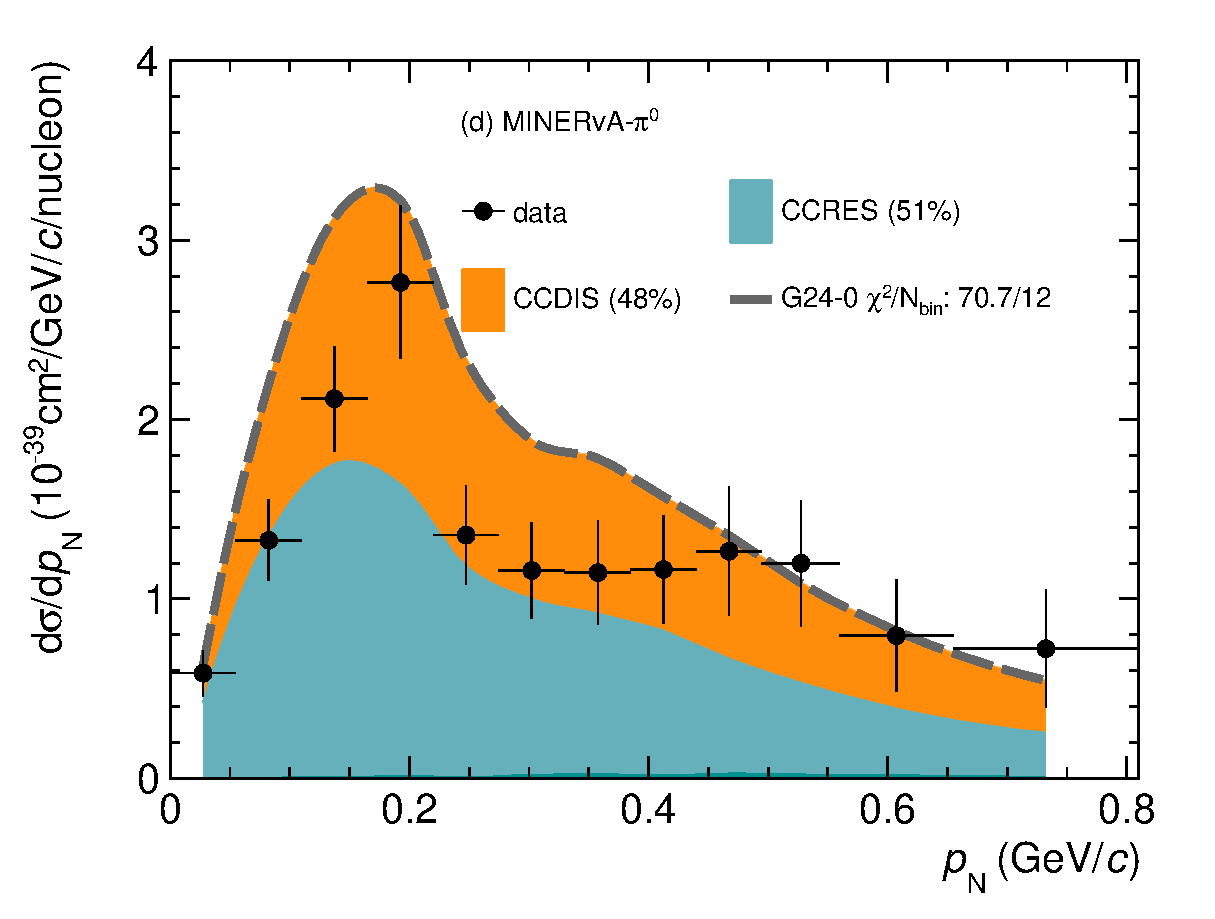
\includegraphics[width=\dbfigwid\textwidth]{figures/0000-min_pi0_pn_reac_decomp.eps}
    \caption{\label{fig:g24-0-pn-reac} Similar to Fig.~\ref{fig:g24-0-dat-reac} but for the $\pn$ (\ttkpip, \minzpi and \minpiz) and $\dpt$ (\ttkzpi) measurements.
    } 
\end{figure*}

\begin{table}[!htb]
    \centering
    \begin{tabular}{cc}
    \hline
    \hline
    Variables & Cuts ($p$ in $\gevc$) \\
    \hline
    \multicolumn{2}{c}{\ttkzpi~\cite{T2K:2018rnz}} \\
    \hline
    $\vecpmu$    &  $0.25 < p_\mu $, $\cos\theta_\mu>-0.6$   \\
    $\vecpp$     & $0.45< p_\text{p} <1.0$ , $\cos\theta_\text{p}>0.4$     \\
    \hline
    \multicolumn{2}{c}{\ttkpip~\cite{T2K:2021naz}} \\
    \hline
    $\vecpmu$    & $0.25 < p_\mu < 7$ , $\theta_\mu < 70^\degree$  \\
    $\vecpp$     & $0.45 < p_\text{p} <1.2$  ,  $\theta_\text{p} < 70^\degree$   \\
    $\vecppi$    & $0.15 < p_\pi <  1.2$, $\theta_\pi < 70^\degree$ \\
    \hline
    \multicolumn{2}{c}{\minzpi~\cite{MINERvA:2018hba, MINERvA:2019ope}} \\
    \hline
    $\vecpmu$     & $1.5< p_\mu < 10$ , $\theta_\mu < 20^\degree $  \\
    $\vecpp$      & $0.45< p_\text{p} <1.2$  , $\theta_\text{p} < 70^\degree$    \\
    \hline
    \multicolumn{2}{c}{\minpiz~\cite{MINERvA:2020anu}} \\
    \hline
    $\vecpmu$   & $1.5< p_\mu < 20$ , $\theta_\mu < 25^\degree$  \\
    $\vecpp$    & $0.45< p_\text{p} $                      \\
    \hline
    \hline
    \end{tabular}
    % \end{ruledtabular}
    \caption{\label{tab:data-sets-phase-space-cut}
    Kinematic cuts for the samples of the TKI measurements.
    }
\end{table}

Given the significant physics potential of TKI measurements, a wealth of literature has emerged on the combined analysis of T2K and MINERvA CC0$\pi$ TKI data~\cite{Dolan:2018zye, Bourguille:2020bvw, Franco-Patino:2021yhd, Ershova:2022jah, Franco-Patino:2022tvv, GENIE:2022qrc, Chakrani:2023htw, Ershova:2023dbv}. However, model studies incorporating TKI data with pion production have been notably absent. Since the TKI measurements are sensitive to the initial state and FSI, this work investigates a partial tune of these two processes, in an effort to derive an effective model describing neutrino-nuclear pion production, while maintaining the efficacy with the pionless production.

\section{\genie model selection}\label{sec:genie}
\genie uses formatted strings to uniquely define configurations, which are usually called tunes. 
Regardless of the name, they can refer to configurations either before or after an actual tuning procedure. 

Free nucleon tuning effort in Ref.~\cite{GENIE:2021zuu} has produced a tune, $\geighteen$, with better description of bubble chamber data. 
This is the starting point of the model we want to tune. 
The first effect to apply to this model is adding the proper initial state. 
Among the available \genie initial state models, the best choice is the spectral-function-like Correlated Fermi Gas model (\sfcfg)~\cite{sfcfg-talk,sfcfg-GitHubCommit,GENIE:2021npt}. 
\sfcfg is essentially based on the previously implemented Local Fermi Gas (LFG) model in \genie with a larger number of adjustable degrees of freedom for tuning and improved physics. 
It differs from the previous implementation of LFG in two aspects. 
``Spectral-function-like'' refers to the implementation of removal energy as a varying function rather than a fixed value, while ``Correlated'' highlights the incorporation of the high-momentum tail above the Fermi momentum due to nucleon-nucleon short-range correlations (SRC), as evidenced by electron-scattering data~\cite{PhysRevLett.96.082501}.
These two improvements are considered and modeled in the Valencia Model in Ref.~\cite{Nieves:2004wx}.
Hence, \sfcfg resembles closer the initial state of the Valencia model than previous LFG implementations.
More details on the \sfcfg can be found in Ref.~\cite{GENIE:2021npt}. 
Note that the original Valencia Model in Ref.~\cite{Nieves:2004wx} has its own method of modeling FSI. 
However, since FSI is factorized from other models in implementation in \genie, this method is not used.
Instead, GENIE develops the INTRANUKE hA FSI model (hA for short) for its simplicity and interpretability, which is the FSI candidate for the model to be tuned in this work.

Further improvements to the configuration to be tuned include: 1) using $z$-expansion axial-vector form factor~\cite{Hill:2010yb} rather than the dipole form factor of the Valencia model in QE processes~\cite{Nieves:2004wx}; and 2) replacing the Valencia model~\cite{Nieves:2011pp} in 2p2h processes with the SuSAv2 Model~\cite{Gonzalez-Jimenez:2014eqa} since it covers larger region of the $q^0$, $q^3$ phase space.

%\sout{Given its simplicity and interpretability, the INTRANUKE hA FSI model (hA for short) emerges as the FSI candidate for the model to be tuned.}
The complete list of the model components are given in Table ~\ref{tab:default-gen-list}. 
In the \genie code, this configuration is identified as \newtune and it is currently the default \genie configuration for a number of LAr based experiments. 
As \newtune is widely used in the paper, we will call it \gZero for simplicity. 

Comparing the \genie predictions for \gZero against TKI datasets, Figs.~\ref{fig:g24-0-dat-reac} and~\ref{fig:g24-0-pn-reac},  shows that the model fails to  accurately describe the MINERvA $\pi^0$~\cite{MINERvA:2020anu} TKI measurement. 

\begin{table}[!htb]
    \centering
    \begin{tabular}{p{4cm}c}
    \hline
    \hline
    \textrm{Simulation component} & \textrm{Model} \\
    \hline
    \textrm{Nuclear state}              & \sfcfg~\cite{sfcfg-talk,sfcfg-GitHubCommit,GENIE:2021npt} \\ 
    \textrm{QE}               & Valencia~\cite{Nieves:2004wx} \\
    \textrm{2p2h}               & SuSAv2~\cite{Gonzalez-Jimenez:2014eqa} \\
    \textrm{QE $\Delta S=1$}           & Pais~\cite{Pais:1971er} \\
    \textrm{QE $\Delta C=1$}                  & Kovalenko~\cite{Kovalenko:1990zi} \\
    \textrm{Resonance (RES)}                        & Berger-Sehgal~\cite{Berger:2007rq}\\
    Shallow/Deep inelastic \par scattering (SIS/DIS)                    & Bodek-Yang~\cite{Bodek:2002vp}\\
    \textrm{DIS $\Delta C=1$}           & Aivazis-Tung-Olness~\cite{Aivazis:1991fy}\\
    \textrm{Coherent $\pi$ production}  & Berger-Sehgal~\cite{Berger:2008xs}\\
    \hline
    \textrm{Hadronization}              & AGKY~\cite{Yang:2009zx}\\
    \textrm{FSI}                        & INTRANUKE hA~\cite{Andreopoulos:2015wxa}\\
    \hline
    \hline
    \end{tabular}
    \caption{\label{tab:default-gen-list} Model components of \gZero. Processes with non-trivial $\Delta S$ and $\Delta C$ are those with strangeness and charm production, respectively.}
\end{table}


\section{\label{sec:Tuning}Tuning initial-state and FSI models on TKI data}

This study adopts the tuning procedure outlined in Ref.~\cite{GENIE:2022qrc}, utilizing $N_{\textrm{par}}$ model parameters. The objective is to identify the best fit---that is, the optimal set of parameter values---within the parameter space that minimizes the $\chi^2$ between model predictions and data. Given the high dimensionality of the parameter space, conducting a brute-force, point-by-point scan on a grid is infeasible. Therefore, a sufficient number of points is randomly sampled. Each point is used to run a full simulation. The simulation output for each data observable bin is then parameterized using Professor~\cite{Buckley:2009bj} with a polynomial of the model parameters of a chosen order, $N_{\textrm{ord}}$. The minimal number of points ($N_{\textrm{s}}$) required for tuning $N_{\textrm{par}}$ parameters with an order $N_{\textrm{ord}}$ polynomial is determined by the combination formula,
\begin{equation}
    N_{\textrm{s}} = \binom{N_{\textrm{par}}+N_{\textrm{ord}}}{N_{\textrm{ord}}}.
\end{equation}
Given that $N_\textrm{s}$ increases factorially, caution is essential when augmenting the number of parameters or the polynomial degree. Given that our tuning incorporates all $2$ \sfcfg and $12$ hA parameters (see Sec.~\ref{sec:tuning-para-choice}), a degree-$4$ parameterization  necessitates over 6,000 generations. Hence, only up to order $4$ polynomials are explored, and it has shown to reproduce the MC predictions well, as shown in Fig.~\ref{fig:residual}. 

\begin{figure}[!htb] 	
    \centering 		
    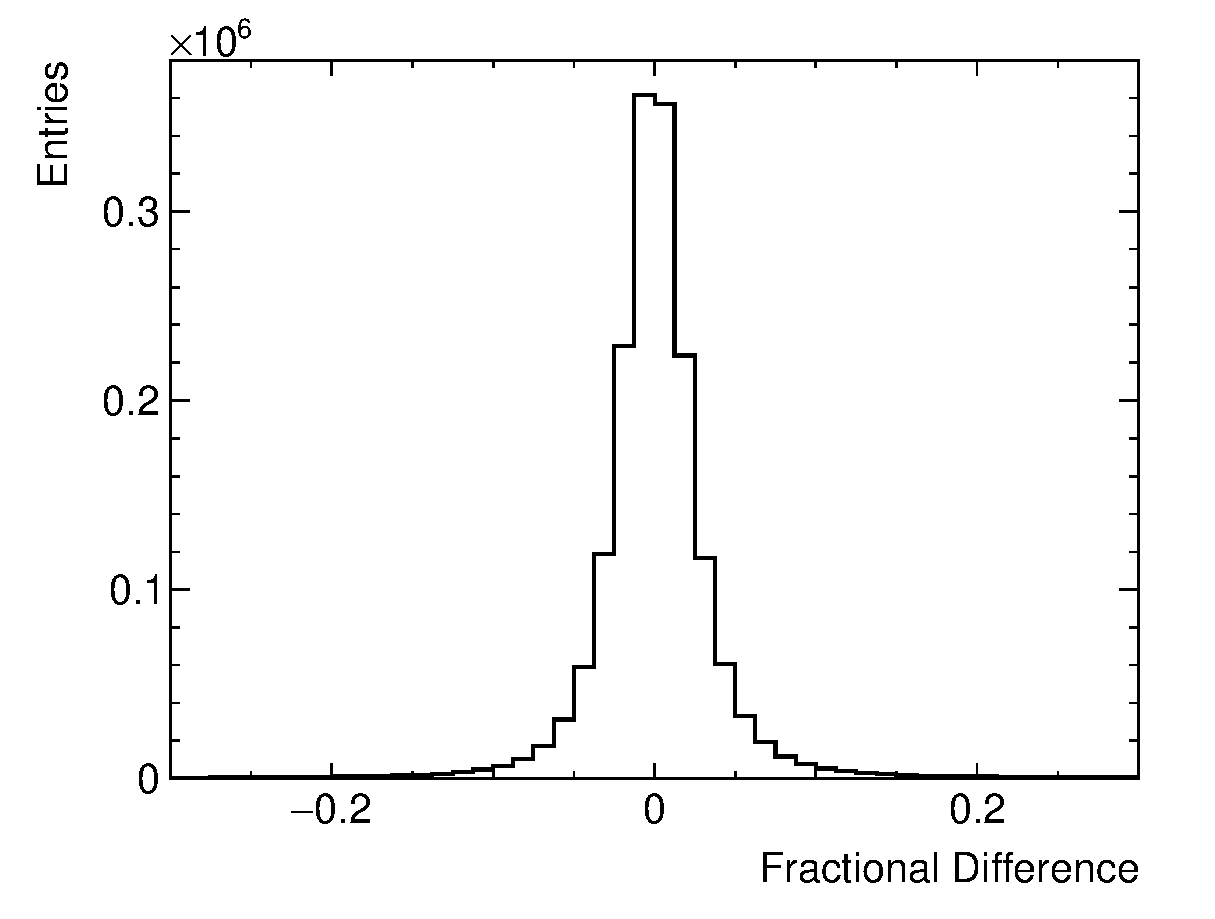
\includegraphics[width=\sgfigwid\textwidth]{figures/residual.eps}
    \caption{\label{fig:residual} Fractional difference for the bin-by-bin cross sections between MC truth and the parameterized approximation with order-4 polynomials,  both in the Norm-Shape (NS)~\cite{DAgostini:1993arp,Hanson:2005mrg} space with \allpar. See Table~\ref{tab:hALFG-para} for the definition of \allpar. The residual has a mean of $0.003$ and a standard deviation of $0.073$.} 
\end{figure}

Furthermore, to circumvent Peelle's Pertinent Puzzle~\cite{PPP_FNL,Chakrani:2023htw}, the Norm-Shape (NS) transformation prescription~\cite{DAgostini:1993arp,Hanson:2005mrg} is applied. The extremal point is then found from a minimization of $\chi^2$ between this NS-transformed polynomial approximation and NS-transformed data. In minimization, priors, usually based on systematic uncertainty, can be imposed on each parameter to penalize it from getting too far from its default value. The following subsections elaborate on the specific choice of measurement observables and model parameters in this work.

\subsection{\label{sec:tuning-obs-choice} Data points}

The observables for the reported differential cross sections across the four TKI measurements---\ttkzpi, \ttkpip, \minzpi, and \minpiz---are detailed in Table~\ref{tab:data-sets}. To identify the most sensitive variables, various combinations were evaluated  for tuning purposes. A total of 26 combinations were assessed,  with the superset comprising $\dat$, $\dpt$, $\dphit$, $\pn$, and $\dptt$ (see Table~\ref{tab:fit-var-combo} in Appendix~\ref{sec:appcombi} for all combinations). Each combination was evaluated such that non-selected variables---including proton momentum and angle ($p_\text{p}$ and $\theta_\text{p}$)~\cite{MINERvA:2018hba}, as well as $\dptx$ and $\dpty$~\cite{MINERvA:2019ope} in \minzpi---were used solely for validation; the model is expected to accurately predict these variables post-tuning. When constructing the combinations, it was observed that $\dphit$ is strongly dependent  on neutrino beam energy~\cite{Lu:2015tcr}, which suppresses its sensitivity to nuclear effects. Additionally, correlations exist between various observables, notably between $\dpt$ and $\pn$. Therefore, determining the optimal combination is not straightforward; this study employs a criterion based on  the $\chi^2$ with the complete (tuned plus validation) observable set (Fig.~\ref{fig:allchi}).


\begin{table}[!htb]
    \centering
    \begin{tabular}{cp{1.1cm}p{1.5cm}p{1.5cm}p{1.5cm}}
    \hline
    \hline
    Observables & No. of \par bins & \texttt{Combi-} \par \texttt{Superset}  & \texttt{Combi-} \par \texttt{Best-} \par \allpar& \texttt{Combi-} \par \texttt{Best-} \par \redpar\\
    \hline
    \multicolumn{5}{c}{\ttkzpi} \\
    \hline
       $\dat$            & $8$                & $\tick$     &  & $\tick$  \\ 
       $\dpt$            & $8$                & $\tick$     & $\tick$  & $\tick$ \\ 
       $\dphit$          & $8$                & $\tick$     &  &  \\      
    \hline
    \multicolumn{5}{c}{\ttkpip} \\
    \hline
      $\dat$            & $3$                & $\tick$      &  & $\tick$  \\
      $\pn$             & $4$                & $\tick$      & $\tick$  & $\tick$ \\ 
      $\dptt$           & $5$                & $\tick$      &  & $\tick$  \\ 
    \hline
    \multicolumn{5}{c}{\minzpi} \\
    \hline  
      $\dat$            & $12$               & $\tick$      & & $\tick$  \\ 
      $\pn$             & $24$               & $\tick$      & $\tick$  & $\tick$ \\
      $\dpt$            & $24$               & $\tick$      & $\tick$ &  \\     
      $\dphit$          & $23$               & $\tick$      &  &  \\     
      $\pp$             & $25$               &      &  &  \\     
      $\thetap$         & $26$               &      &  &  \\     
      $\dptx$           & $32$               &      &  &  \\  
      $\dpty$           & $33$               &      &  & \\     
    \hline
    \multicolumn{5}{c}{\minpiz} \\
    \hline
      $\dat$            & $9$               & $\tick$      & & $\tick$      \\  
      $\pn$             & $12$               & $\tick$     & $\tick$  & $\tick$ \\ 
      $\dptt$           & $13$               & $\tick$     &  & $\tick$  \\
    \hline
    \hline
    \end{tabular}
    \caption{\label{tab:data-sets}
	(NEW) Observables of the TKI measurements and their binning. Those with ``$\tick$'''s are used for tuning, while those without  are for the respective validation. See Table~\ref{tab:hALFG-para} for definitions of \cbRedPar and \cbAllPar.
    }
\end{table}



\begin{figure}[!htb] 
    \centering 		
    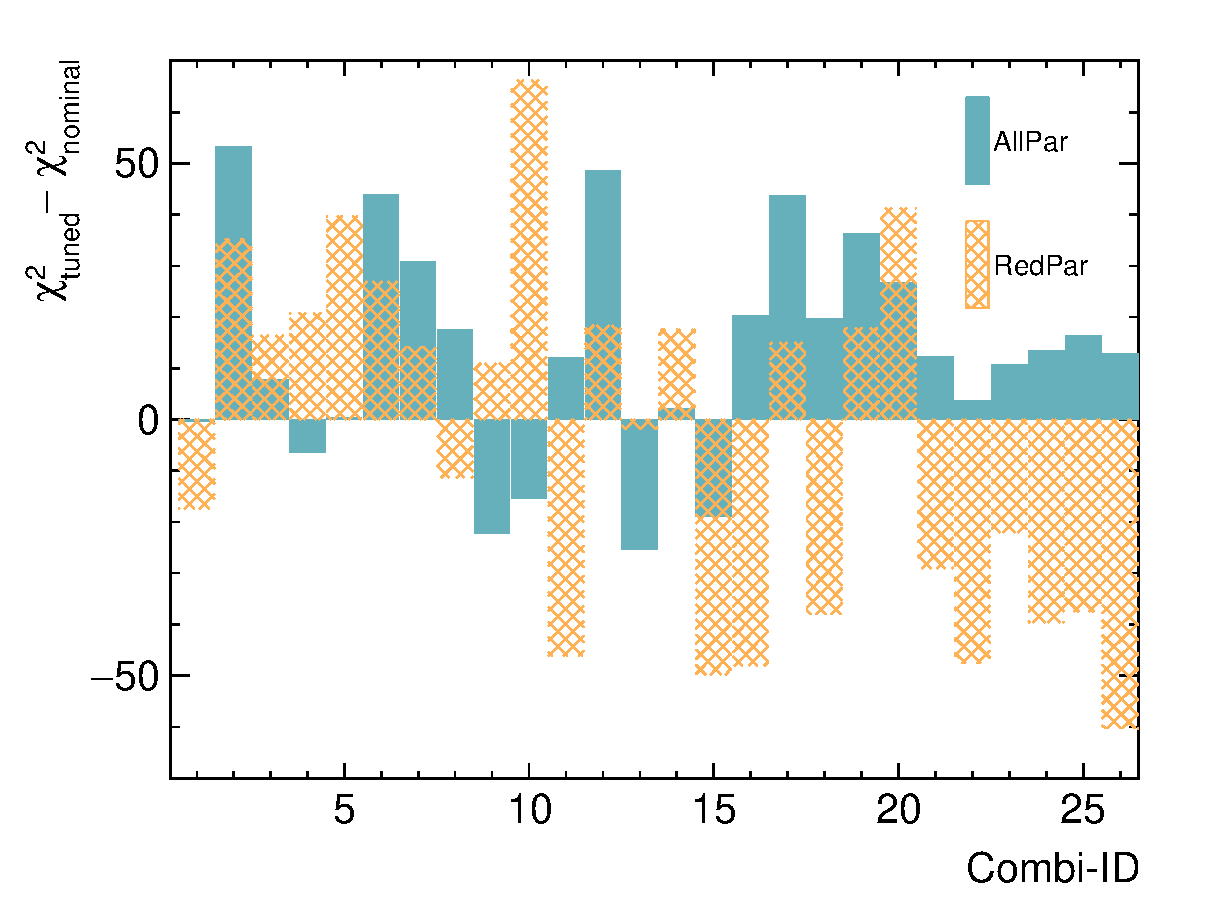
\includegraphics[width=\sgfigwid\textwidth]{figures/chi2_hist_covfix.eps} 
    \caption{\label{fig:allchi} Change of $\chi^2$ calculated for the full (i.e., tuned plus validation) observable set as a function of the tuned combination (cf. Table~\ref{tab:fit-var-combo} in Appendix~\ref{sec:appcombi}). The two model parameter sets (\allpar and \redpar, see Table~\ref{tab:hALFG-para} for definitions) are compared and it can be seen that the respective minima happen at \texttt{Combi-15} and 26. }   
\end{figure}

\subsection{\label{sec:tuning-para-choice} Model parameters}
As outlined in Sec.~\ref{sec:genie}, we focus exclusively on the currently tunable parameters within the \sfcfg and hA models. Therefore, $14$ parameters (collectively referred to as the \allpar set) are utilized for tuning, as detailed in Table~\ref{tab:hALFG-para}. Nominal values and associated uncertainties for the hA model are taken from Table 17.3 in Ref.~\cite{Andreopoulos:2015wxa}. 

\begin{table}[!htb]
    \centering
    \begin{tabular}{cp{1.5cm}p{1.5cm}p{1.2cm}p{1.2cm}}
    \hline
    \hline
    \textrm{Parameter} & \textrm{Nominal} (\gZero)     & \textrm{Range In} \par \textrm{Tuning} & \allpar \par (\gT)  & \redpar \par (\gC) \\ 
    \hline
    \multicolumn{5}{c}{\sfcfg} \\
    \hline
    \textrm{$\srcfr$} & 0.12 & (0.0, 0.5)  & \tick & \tick\\
    \textrm{$\nurmec$} & 0.01 & (0.0, 0.2) & \tick & \\
    \hline
    \multicolumn{5}{c}{hA} \\
    \hline
    \textrm{$\cpimfp$} & $1.0\pm0.2$ & (0.0, 3.0) & \tick & \\
    \textrm{$\pizmfp$} & $1.0\pm0.2$ & (0.0, 3.0) & \tick & \tick\\
    \textrm{$\nmfp$} & $1.0\pm0.2$ & (0.0, 3.0) & \tick &\\
    \hline
    \textrm{$\picex$} &  $1.0\pm0.5$ & (0.0, 3.0) & \tick & \tick \\
    \textrm{$\ncex$} & $1.0\pm0.5$ & (0.0, 3.0)  & \tick & \tick\\
    \hline
    \textrm{$\piinel$} & $1.0\pm0.4$ & (0.0, 3.0) & \tick & \\
    \textrm{$\ninel$} & $1.0\pm0.4$ & (0.0, 3.0)  & \tick &\\
    \hline
    \textrm{$\cpiabs$} & $1.0\pm0.2$ & (0.0, 3.0) & \tick &\\
    \textrm{$\pizabs$} & $1.0\pm0.2$ & (0.0, 3.0) & \tick &\\
    \textrm{$\nabs$} & $1.0\pm0.2$ & (0.0, 3.0)  & \tick & \tick\\
    \hline
    \textrm{$\pipiprod$} & $1.0\pm0.2$ & (0.0, 3.0) & \tick &\\
    \textrm{$\npiprod$} & $1.0\pm0.2$ & (0.0, 3.0)  & \tick & \tick\\
    \hline
    \hline
    \end{tabular}
    \caption{\label{tab:hALFG-para}
    Tuneable parameters and their ranges in the  \sfcfg (\textit{uppermost} group) and hA (\textit{lower} groups, uncertainties from Ref.~\cite{Andreopoulos:2015wxa}) models. Parameters to be tuned in the two sets are marked with ``\tick'''s. See later text for definitions of \gT and \gC.
    }
\end{table}

In our analysis of the \sfcfg model, the two most relevant parameters are $\srcfr$, representing the fraction of the high-momentum tail from SRC, notably above the Fermi surface, and $\nurmec$, marking the commencement of the nuclear removal energy distribution for carbon. A larger $\srcfr$ indicates the presence of more energetic initial nucleons, while an increased $\nurmec$ implies that greater energy is necessary to liberate a nucleon from the carbon nucleus, so the product particles will possess lower energy. Given the novelty and limited constraints of the spectral-function-like implementation, this study employs relatively relaxed priors for $\srcfr$ and $\nurmec$, at 0.12$\pm$0.12 and 0.01$\pm$0.005 \gev, respectively.

\genie users employ the hA model~\cite{Andreopoulos:2015wxa} for the majority of neutrino analysis, owing to its straightforward reweighting capability. Unlike cascade models such as the hN model~\cite{Andreopoulos:2015wxa}, this model determines the FSI type for each hadron exactly once, without considering further propagation of rescattered hadrons within the nucleus. Its model parameters are explained as follows.

\begin{enumerate}
    \item 
The model evaluates a mean free path (MFP), $\lambda$, which varies with the hadron's energy, $E$, and its radial distance, $r$, from the nucleus center,  as follows:
\begin{equation}
    \lambda(E,r) = \frac{1}{\sigma_\textrm{hN,tot}(E)\rho(r)},
\end{equation}
where $\sigma_\textrm{hN,tot}$ is the total hadron-nucleon cross section and $\rho$ is the number density of the nucleons inside the nucleus. Once a hadron is generated inside the nucleus, it travels a distance $\lambda$ before a probabilistic determination of rescattering occurs, inversely related to  $\lambda$. If no rescattering happens, the hadron will be propagated for another $\lambda$ and the dice will be thrown again. The cycle repeats until a rescattering happens or the hadron is propagated far enough to escape the nucleus without any interactions. If a rescattering happens, the type of rescattering is evaluated according to their cross section. The relative probabilities of each type are extracted from stored hadron scattering data~\cite{LADS:1999dyv,Navon:1983xj,Carroll:1976hj,Clough:1974qt,BAUHOFF1986429,Mashnik:2000up,Ishibashi:1997gbe}. After a specific rescattering type is chosen, the rescattered product will be generated. These rescattered products will not undergo further rescattering and will be considered out of the nucleus as final state particles.  
The MFP values for pions and nucleons can be modified using scaling factors  ($\cpimfp$, $\pizmfp$,  and $\nmfp$) detailed in Table~\ref{tab:hALFG-para}. Both changed pions, $\pip$ and $\pim$, are scaled by the same factor, $\cpimfp$, due to isospin symmetry. The $\lambda$ for $\piz$ is calculated from those of charged pions based on isospin symmetry as well and can be adjusted separately by $\pizmfp$. If the factor is larger than $1$, $\lambda$ will increase and hence the total number of steps required for the hadron to escape the nucleus reduces, thereby reducing the average probability of rescattering. 
Given the high precision with which total hadron-nucleus cross sections are determined~\cite{LADS:1999dyv,Navon:1983xj,Carroll:1976hj,Clough:1974qt,BAUHOFF1986429}, strict Gaussian priors (error---$\sigma$, not to be confused with the various cross sections---of $0.2$, same as the systematic uncertainties shown in Table~\ref{tab:hALFG-para}) are applied to the MFP scaling factors. 
Varying $\pizmfp$ by $\pm2.5~\sigma$ significantly affects the \minpiz $\textrm{d}\sigma/\textrm{d}\pn$, as depicted in Fig.~\ref{fig:minpiz-pn-pi0mfp}. Decreasing MFP naturally leads to increased rescattering. Hence, fewer $\piz$s can escape the nucleus and fewer events will have $\piz$ in the final states, thereby reducing the cross section. 

\begin{figure}[!htb]
    \centering
    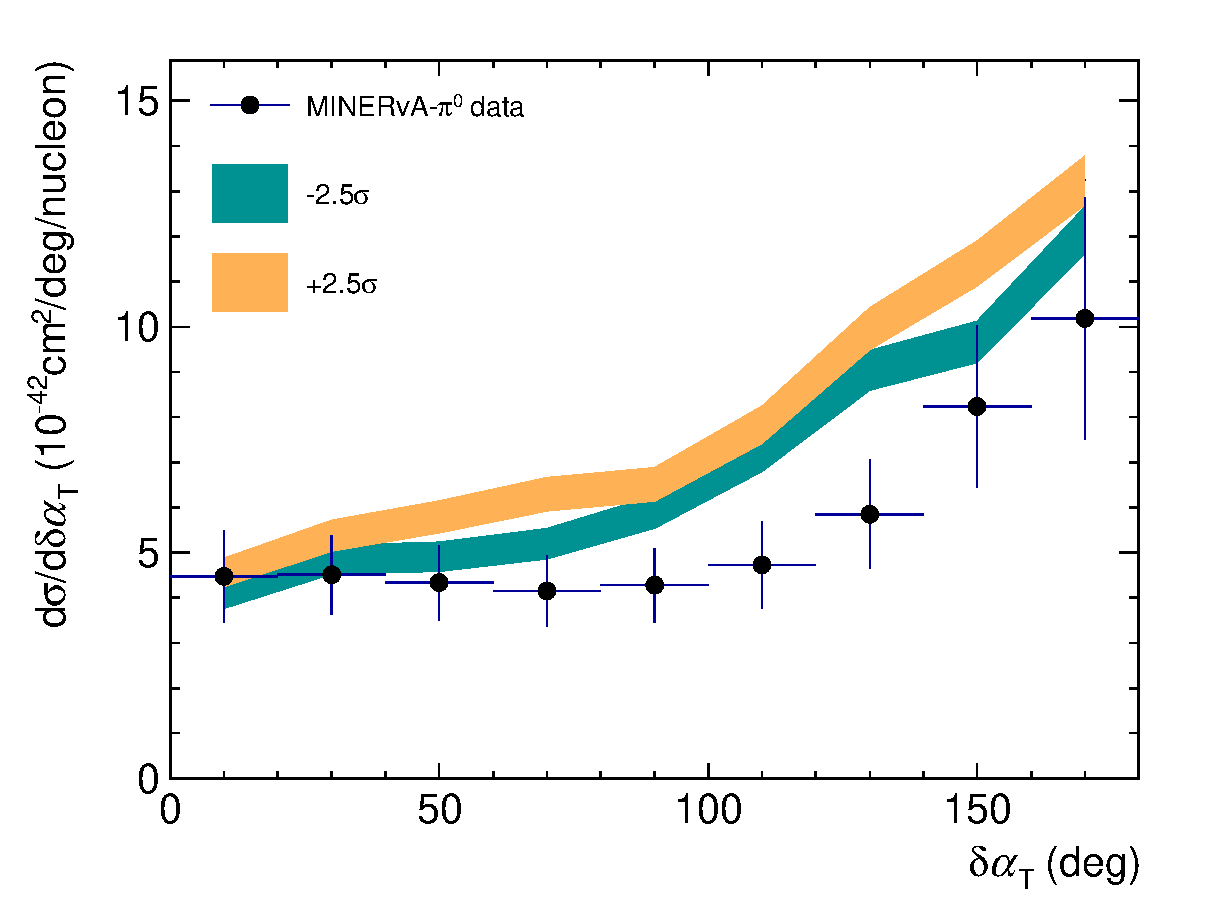
\includegraphics[width=\dbfigwid\textwidth]{figures/minerva_pi0_dalphat_FSI_pi0mfp.eps}
    \caption{Effect of varying $\pizmfp$ by $\pm2.5~\sigma$ compared to the MINERvA-$\pi^0$ measurement. Each band's width indicates the \genie prediction's statistical uncertainty from $10^5$ events.}
    \label{fig:minpiz-pn-pi0mfp}
\end{figure}


\item 
The relative probability of each rescattering type can be adjusted by a scale factor. There are four rescattering types for both nucleons and pions available for tuning. They are charge exchange (CEX), inelastic scattering (INEL), absorption (ABS), and pion production (PIPD). The default energy-dependent probability distributions come from hadron data tuning~\cite{LADS:1999dyv,Navon:1983xj,Carroll:1976hj,Clough:1974qt,BAUHOFF1986429} and can be adjusted by respective scaling factors, like $\picex$ for CEX of all pions, listed in Table~\ref{tab:hALFG-para}. The relative probabilities of all four rescattering types will be normalized such that they sum up to one. Scaling factors directly multiply  the probability of each type, with new relative probabilities subsequently renormalized. More specifically, suppose the initial fraction of absorption, $f_\textrm{ABS}$, is $0.5$, which means that the sum of the other fractions is  $f_\textrm{other}=f_\textrm{INEL}+f_\textrm{CEX}+f_\textrm{PIPD}=1-0.5=0.5$. If $f_\textrm{ABS}$ is scaled up with $S_\textrm{ABS}=2$, the new absorption fraction is 
\begin{equation}
    f^\prime_\textrm{ABS} = \frac{f_\textrm{ABS}*S_\textrm{ABS}}{f_\textrm{ABS}*S_\textrm{ABS}+f_\textrm{oth}} = 2/3,
\end{equation}
which is not equal to simply multiplying $f_\textrm{ABS}$ by $S_\textrm{ABS}$ due to the presence of the other rescattering types. Hence, it is unavoidable that a change of the scaling factor for one type would affect others. Nonetheless, when the cross section is plotted with a breakdown according to rescattering type, the interpretation will be clear regarding the increase or decrease of a particular FSI type. This correlation implies that the scaling parameters' effective impact on FSI fate is often less pronounced than what the raw numbers suggest. As illustrated in the above example, $f_\textrm{ABS}$ is only scaled up by $ f^\prime_\textrm{ABS}/f_\textrm{ABS}=4/3=1.3$ instead of $S_\textrm{ABS}=2$. Hence, a relatively more relaxed Gaussian prior, with a $\sigma$ of $0.5$, is placed on the FSI fate scales, slightly larger than the systematic uncertainties shown in Table~\ref{tab:hALFG-para}. 

Understanding each rescattering type is crucial for interpreting tuning results. A detailed elaboration of the four tunable FSI types is given as follows. 

\begin{enumerate}
    \item 
CEX involves changing the charge of the participating particles; for example,
\begin{equation}
    \pip + \n \rightarrow \piz + \p,
\end{equation}
or vice versa. This rescattering type is crucial for event topologies requiring the presence of a pion;  depending on the signal pion charge, CEX could migrate events between signal and background. 

\item 
INEL is the case where the nucleus is left in an excited state after the rescattering. This category only contains the situation where a single additional nucleon is emitted/knocked-out after rescattering. Since it does not affect the number of pions produced, it will not convert an event from a pionless topology to a pion-production topology. The effects on nucleons are two-fold. Firstly, it can alter the number of signal events within each event topology. If the inelastic rescattering leads to two low-momentum protons below the detection threshold as opposed to a high-momentum proton, this signal event will be discarded as no protons are observed. Secondly, INEL invariably changes the kinematics of the rescattering particle. Be it the leading proton or the leading pion, based on which the TKI observables are calculated, the TKI distribution shape will be affected. Hence, while $\ninel$ would affect all four data sets, $\piinel$ would only affect \ttkpip and \minpiz. 

\item 
ABS refers to the case where the particle undergoes an interaction so that it does not emerge as a final particle. For example, $\pi^+$ can interact with two or more nucleons, initially forming a baryon resonance that subsequently interacts with other nucleons, emitting multiple nucleons rather than pions. Hence, the $\pi^+$ would not emerge from the nucleus anymore.

\item 
PIPD happens for energetic particles where an extra pion emerges as a result of the rescattering, such as
\begin{equation}
    \p + \p \rightarrow \p + \n + \pip.
\end{equation}
Such an interaction significantly alters the event topology. 

\end{enumerate}
\end{enumerate}

\section{\label{sec:results}The first TKI-driven \genie tunes}

% \begin{figure}[!htb] 	
%     \centering 		
%     \setkeys{Gin}{width=\linewidth}
%     \begin{subfigure}{width=\dbfigwid\textwidth}
%     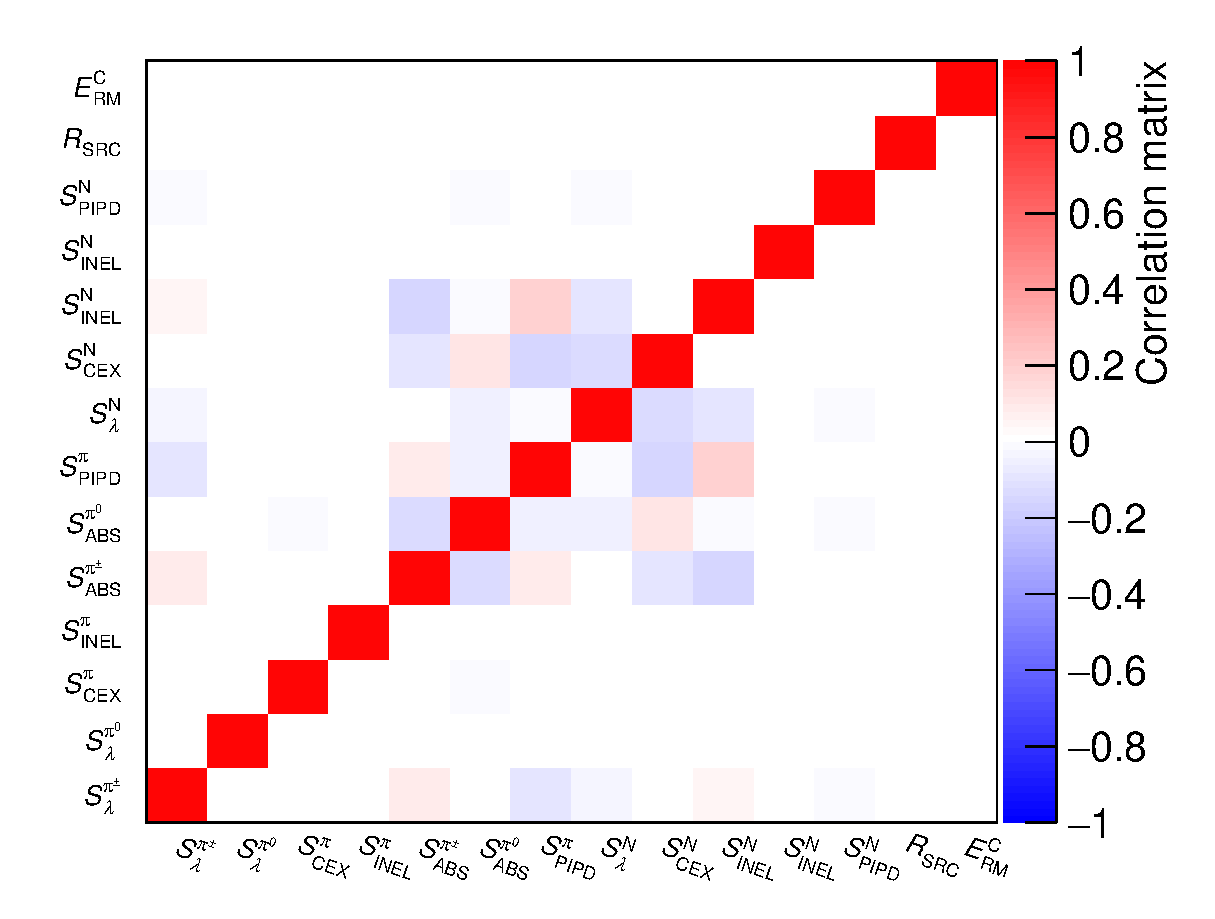
\includegraphics{figures/result_test_comb_26_cor_allpar.eps}
%     \subcaption{\label{fig:comb_26_cor_allpar}\allpar}
%     \end{subfigure}
%     \begin{subfigure}{width=\dbfigwid\textwidth}
%     \includegraphics{figures/result_test_comb_26_cor_redpar.eps}
%     \subcaption{\label{fig:comb_26_cor_redpar}\redpar}
%     \end{subfigure}
%     \caption{ Post-fit Correlation coefficient on \texttt{Combi-26}. } 
% \end{figure}

\begin{figure}[!htb] 	
    \centering 		

    \includegraphics[width=\dbfigwid\textwidth]{figures/result_test_comb_26_cor_allpar.eps}
    \includegraphics[width=\dbfigwid\textwidth]{figures/result_test_comb_26_cor_redpar.eps}
    \caption{ Post-fit Correlation coefficient on \texttt{Combi-26}. } 
\end{figure}

\begin{figure*} 
    \centering 		
    \includegraphics[width=\dbfigwid\textwidth]{figures/0026-t2k_0pi_dalphat_reac_decomp.eps}
    \includegraphics[width=\dbfigwid\textwidth]{figures/0026-t2k_pip_dalphat_reac_decomp.eps}
    \includegraphics[width=\dbfigwid\textwidth]{figures/0026-min_0pi_dalphat_reac_decomp.eps}
    \includegraphics[width=\dbfigwid\textwidth]{figures/0026-min_pi0_dalphat_reac_decomp.eps}
    \caption{\label{fig:g24-c-dat-reac} 
    Similar to Fig.~\ref{fig:g24-0-dat-reac} but with \gC.  The \gZero prediction is also plotted for comparison. 
    } 

    \includegraphics[width=\dbfigwid\textwidth]{figures/0026-t2k_0pi_dpt_reac_decomp.eps}
    \includegraphics[width=\dbfigwid\textwidth]{figures/0026-t2k_pip_pn_reac_decomp.eps}	
    \includegraphics[width=\dbfigwid\textwidth]{figures/0026-min_0pi_pn_reac_decomp.eps}
    \includegraphics[width=\dbfigwid\textwidth]{figures/0026-min_pi0_pn_reac_decomp.eps}
    \caption{\label{fig:g24-c-pn-reac}  
    Similar to Fig.~\ref{fig:g24-c-dat-reac} but for the $\pn$ (\ttkpip, \minzpi and \minpiz) and $\dpt$ (\ttkzpi) measurements. 
    } 
\end{figure*}

Given the intricate correlations among model parameters, determining which ones are most sensitive to the data proves challenging. Considerable correlation and anti-correlation are observed between different FSI fates for the same particle, e.g. $\cpiabs$ and $\picex$, as shown in Figs.~\ref{fig:comb_26_cor_allpar} and~\ref{fig:comb_26_cor_redpar}. 
Our tuning began with the \allpar parameter set, achieving the best result with \texttt{Combi-15}, which is denoted as \cbAllPar in Table~\ref{tab:data-sets} (cf. Fig.~\ref{fig:allchi} for the $\chi^2$ distribution of all combinations).
Observations showed that for most combinations, certain parameters remained close to their default values, within $1$ $\sigma$ of the imposed priors, such as $\pipiprod$ since none of the data sets has a significant contribution from PIPD of pions---Removing these parameters from the tuning process does not significantly affect the outcome.
Therefore, we then constructed a reduced set comprising only $\srcfr$, $\pizmfp$, $\picex$, $\ncex$, $\nabs$, and $\npiprod$ (denoted as \redpar in Table~\ref{tab:hALFG-para}) and ran the tuning on the 26 combinations with it. Note that the parameters most correlated with $\picex$ and $\pizmfp$ are not present in \redpar. The \redpar tuning proved more stable, with nearly all combinations showing a more negative $\chi^2$ change than the \allpar tuning, as shown in Fig.~\ref{fig:allchi}. Moreover, the single-observable (\texttt{Combi-}1 to 5), single-measurement (\texttt{Combi-}6 to 9), single-experiment (\texttt{Combi-}10 and 11), and single-topology (\texttt{Combi-}12 and 13) combinations all systematically yielded no or limited overall (tuned plus validation) improvement post-tuning. The best tuning then occurred with \texttt{Combi-26} (\cbRedPar in Table~\ref{tab:data-sets}), that is, all TKI variables excluding $\dphit$ and $\dpt$ (unless no $\pn$ is available)---$\dat$, $\pn$ (or $\dpt$ if $\pn$ is unavailable), and $\dptt$---from pionless and pion-production measurements in both T2K and MINERvA. 

Table~\ref{tab:restunes} summarizes the primary results of our tuning process. The tuned \redpar, \restunefull (\gC), is derived from the observable set \cbRedPar, and the tuned \allpar, $\alttune$~(\gT), is from \cbAllPar. The upper part of Table~\ref{tab:restunes} contains the parameter values. For the  \gC tune, changes to the \sfcfg model were moderately sized ($\srcfr$ increases from $0.12$ to $0.15$), while in the hA model, $\pizmfp$ and $\picex$ are highly suppressed and the nucleon FSI has larger CEX and PIPD and lower ABS.  The tune \gT differs most significantly from \gC in $\srcfr$ and $\picex$. The table's lower section illustrates $\chi^2$ improvements for selected observables and their corresponding validation sets. Crucially, tuning should also enhance the accuracy of validation set descriptions. Overall, both tunes have substantial reduction in the total $\chi^2$. In the following, we will discuss the two tunes.

\begin{table}[!htb]
    \centering
    \begin{tabular}{p{1.5cm}p{1.5cm}p{2.1cm}p{2.3cm}}
    \hline
    \hline
    Parameter              & Nominal \par (\gZero) &  \redpar \par (\gC)     & \allpar \par (\gT)   \\
    \hline
    \multicolumn{4}{c}{\sfcfg} \\
    \hline
    $\srcfr$   & 0.12 & 0.09 $\pm$ 0.08         & 0.17  $\pm$ 0.10       \\
    $\nurmec$  & 0.01 & 0.01                    & 0.06 $\pm$ 0.000004     \\
    \hline
    \multicolumn{4}{c}{hA} \\
    \hline
    $\cpimfp$  & $1.0\pm0.2$ & 1.0                      & 1.21   $\pm$ 0.15         \\
    $\pizmfp$  & $1.0\pm0.2$ & 0.34 $\pm$ 0.11          & 0.91   $\pm$ 0.000004     \\
    $\nmfp$    & $1.0\pm0.2$& 1.0                       & 0.89   $\pm$ 0.000382     \\
    \hline
    $\picex$   & $1.0\pm0.5$ & 0.27 $\pm$ 0.28          & 0.86   $\pm$ 0.000056      \\
    $\ncex$    & $1.0\pm0.4$ & 1.39 $\pm$ 0.33          & 0.92  $\pm$ 0.001178       \\
    \hline
    $\piinel$  & $1.0\pm0.4$ & 1.0                      & 0.90   $\pm$ 0.00008       \\
    $\ninel$   & $1.0\pm0.4$ & 1.0                     & 0.92   $\pm$ 0.001218       \\
    \hline
    $\cpiabs$  & $1.0\pm0.2$ & 1.0                      & 1.36   $\pm$ 0.38          \\
    $\pizabs$  & $1.0\pm0.2$ & 1.0                      & 0.92   $\pm$  0.000024     \\
    $\nabs$    & $1.0\pm0.2$ & 0.48 $\pm$ 0.33          & 1.02   $\pm$ 0.413668      \\
    \hline
    $\pipiprod$& $1.0\pm0.2$ & 1.0                      & 1.11   $\pm$ 0.342484       \\
    $\npiprod$ & $1.0\pm0.2$ & 1.90 $\pm$ 0.71          & 1.12   $\pm$ 0.57198        \\ 
    \hline
    \hline
    \multicolumn{4}{c}{$\chi^2$ \textrm{for} \texttt{combi}} \\
    \hline
    \texttt{untuned}         & & 231.75         & 129.61        \\
    \texttt{tuned}           & & 168.67         & 131.46        \\
    \texttt{diff}            & & -63.08         & 1.85         \\
    \hline
    \multicolumn{4}{c}{$\chi^2$ \textrm{for} \texttt{vald}} \\
    \hline
    \texttt{untuned}    & & 229.5          & 331.64        \\
    \texttt{tuned}            & & 232.3    & 304.4         \\
    \texttt{diff}       & & 2.8          & -27.24        \\
    \hline
    \multicolumn{4}{c}{$\chi^2$ \textrm{for} \texttt{combi+vald}} \\
    \hline
    \texttt{untuned}    & &  461.25          &  461.25        \\
    \texttt{tuned}          &  & 400.97 & 435.86        \\
    \texttt{diff} & & -60.28         & -25.39  \\     
    \hline
    \hline
\end{tabular}
\caption{\label{tab:restunes}
	Parameters in \gZero, \gC, and \gT. Those without errors are not tuned. Lower section: \texttt{combi} indicates that the following $\chi^2$ sums are calculated for the tuned measurements (i.e. \cbRedPar (98 bins) and \cbAllPar (72 bins) for \gC and \gT, respectively), while \texttt{vald} indicates that the respective validation sets are used; \texttt{untuned} means that the $\chi^2$ calculation uses the nominal values of the parameters, while \texttt{tuned} denotes the tuned ones. \texttt{diff} displays the improvement achieved by the respective tuning.  
}
\end{table}


\subsection{Reduced tune: \gC}

To assess the tune's quality, we plot predictions using \gC for $\dat$ and $\pn$ in Figs.~\ref{fig:g24-c-dat-reac} and~\ref{fig:g24-c-pn-reac},  respectively. For \ttkzpi, \ttkpip and \minzpi, the new $\chi^2$ values are comparable to those obtained with \gZero, changing less than the number of bins. For \minpiz, \gC is distinctly better than \gZero, thereby demonstrating the possibility of simultaneous good descriptions of both pionless and pion production samples with constrained parameters from cross-topology TKI tuning. Note that in the region of $\pn\sim0.3~\gevc$, the model deficit previously reported in Ref.~\cite{MINERvA:2018hba} (and also shown in Fig.~\ref{fig:g24-0-pn-reac}c) persists even after the fit. The physical origin of this deficit might be attributed to the strength of the 2p2h contribution~\cite{MINERvA:2018hba}, but it is still a topic of significant discussion within the community.

Examining individual datasets closely helps to understand the origin of the improvement. The decomposition of the cross section for $\dat$ according to the FSI fates of the $\piz$ is presented in Fig.~\ref{fig:CEX-minpiz-dat-pi0}. The hA model rescatters primary interaction products only once, and records this event with a rescattering code for these particles. The rescattered products, which are the final outputs, are stored as daughters of the primary interaction products. Hence, the FSI fate that produces the final products can be checked by the rescattering code of their first parent. More specifically, we loop through all final-state particles to look for the leading $\piz$ and check the rescattering code of its first parent. 

\begin{figure}[!htb] 	
    \centering 		
    \includegraphics[width=\dbfigwid\textwidth]{figures/0000-min_pi0_dalphat_pi0_decomp_cex.eps}
    \includegraphics[width=\dbfigwid\textwidth]{figures/0026-min_pi0_dalphat_pi0_decomp.eps}	
    \caption{\label{fig:CEX-minpiz-dat-pi0} \minpiz $\dat$ measurement compared to \genie predictions decomposed in $\piz$ FSI fates with (a) \gZero and (b) \gC.} 
\end{figure}

In \minpiz, the number of $\piz$s undergoing no FSI (``No Interaction'', as shown in the figures) is adjustable via the $\pizmfp$ parameter. A decrease in $\pizmfp$ reduces the size of the ``No Interaction'' events,  as is shown in Fig.~\ref{fig:CEX-minpiz-dat-pi0}b when compared to Fig.~\ref{fig:CEX-minpiz-dat-pi0}a. Meanwhile, an increase in $\piz$ rescattering only manifests in pionless measurements through ABS. There is indeed an increase of ABS for $\piz$ in \ttkzpi and \minzpi, but the fraction is small to begin with, so the impact is small. The increase of $\piz$ rescattering can increase \ttkpip via CEX as discussed below. However, due to the significant suppression of CEX, its impact on \ttkpip is also minimal (for detailed breakdown, see Figs.~\ref{fig:g24-0-dat-pi0}-\ref{fig:g24-c-pn-pi0} in Appendix~\ref{sec:appfate}). 

As shown in Fig.~\ref{fig:CEX-minpiz-dat-pi0}a, the \minpiz prediction from the nominal tune has considerable contributions from CEX controlled by $\picex$. It does not impact \ttkzpi and \minzpi as CEX only changes the pion type without removing them. Hence, events with pions in the final state would be rejected in these two data sets regardless of the pion charge. In principle, CEX will also migrate events between the signal and background definitions for \ttkpip when a $\piz$ is converted to a $\pip$ and vice verse. However, \ttkpip does not have a considerable CEX fraction to begin with, so changing CEX will have a minimal impact on its prediction. Hence, this is one of the most effective paths to decrease the \minpiz cross section prediction without affecting other measurements, and indeed the $\picex$ is heavily suppressed as shown in Table~\ref{tab:restunes} and illustrated in Fig.~\ref{fig:CEX-minpiz-dat-pi0}b compared to Fig.~\ref{fig:CEX-minpiz-dat-pi0}a. However, due to the intricate correlation between the FSI fates in the hA implementation discussed in Sec.~\ref{sec:tuning-para-choice}, although $\piinel$ and $\pipiprod$ are not modified explicitly, a considerable increase is observed in both INEL and PIPD for \minpiz. 

Suppressing both ``No Interaction'' and CEX for $\piz$ adjusts the \minpiz prediction to the appropriate magnitude with small impacts on other data sets.  The effects of the other parameter changes are more transparent in the comparison of the $\pn$ distribution of \minpiz between Figs.~\ref{fig:minpiz-pn-pr}a and~\ref{fig:minpiz-pn-pr}b. A relatively large increase in $\ncex$ and $\npiprod$ moves events away from the Fermi motion peak at $\pn\leq0.25~\textrm{GeV}/c$; the same effect can be achieved by an increased $\srcfr$. 

Another impact of the larger $\npiprod$ manifests in the appearance of 2p2h ($1\%$) and CCQE ($2 \%$) in the \minpiz cross section, as shown in Fig.~\ref{fig:g24-c-pn-reac}d. These neutrino-nucleon interactions do not produce pions, but the product nucleons can produce pions via re-scattering in the nucleus, leading to a contribution to topologies with pions in the final states. However, such contribution remains small.

\begin{figure}[!htb] 	
    \centering 		
    \includegraphics[width=\dbfigwid\textwidth]{figures/0000-min_pi0_pn_pr_decomp_cex.eps}
    \includegraphics[width=\dbfigwid\textwidth]{figures/0026-min_pi0_pn_pr_decomp.eps}	
    \caption{\label{fig:minpiz-pn-pr} Similar to Fig.~\ref{fig:CEX-minpiz-dat-pi0} but for $\pn$ with proton FSI fate decomposition. Note that the ``Absorption'' of the proton is referring to the absorption of the $\pip$ from the decay of $\deltapp$, which could lead to emission of nucleons as discussed in Sec.~\ref{sec:tuning-para-choice}.     
    } 
\end{figure}

Although the interaction models, e.g. 2p2h, are not directly tuned, the respective fractions have undergone small changes in Fig.~\ref{fig:g24-c-dat-reac} and Fig.~\ref{fig:g24-c-pn-reac}, compared to Fig.~\ref{fig:g24-0-dat-reac} and Fig.~\ref{fig:g24-0-pn-reac}. 
This is a result of the increased $\srcfr$ which leads to more events with higher initial nucleon momenta such that interactions requiring higher initial state energy, such as RES and DIS, will be more frequent. 
This is reflected by the increase in the ratios of these interactions: For example, RES increases from $19\%$ (Fig.~\ref{fig:g24-0-pn-reac}c) to $25\%$ (Fig.~\ref{fig:g24-c-pn-reac}c) for \minzpi. 
Hence, the other interactions, although not directly tuned, will experience a decrease in the fraction of total cross section: For example, 2p2h drops from $34\%$ (Fig.~\ref{fig:g24-0-pn-reac}c) to $30\%$ (Fig.~\ref{fig:g24-c-pn-reac}c) for \minzpi.



\subsection{Alternative tune: \gT}

A similar improvement is achieved by the intermediate tune, \gT, illustrated in Fig.~\ref{fig:minpiz-alttune}. Instead of significantly increasing proton PIPD to elevate the $\pn$ tail, this tune notably enhances $\srcfr$---more-energetic nucleons are present and therefore the RES $\pn$ peak is shifted to the right in Fig.~\ref{fig:minpiz-alttune}a with respect to Fig.~\ref{fig:g24-c-pn-reac}d. Rather than suppressing $\picex$ (cf. Fig.~\ref{fig:g24-c-pn-pi0}d in Appendix~\ref{sec:appfate}), this tune significantly increases it (Fig.~\ref{fig:minpiz-alttune}b) to offset the further reduction of ``No Interaction'' $\piz$ events (smaller $\pizmfp$ in \allpar, cf. Table~\ref{tab:restunes}).  Overall, this leads to a reduction of $75.31$ in $\chi^2$ (Table~\ref{tab:restunes}), similar to \gC, as well as a good data-MC agreement across all data sets. 


\begin{figure}[!htb] 	
    \centering 		
    \includegraphics[width=\dbfigwid\textwidth]{figures/0015-min_pi0_pn_reac_decomp_comp.eps}
    \includegraphics[width=\dbfigwid\textwidth]{figures/0015-min_pi0_pn_pi0_decomp_comp.eps}
    \includegraphics[width=\dbfigwid\textwidth]{figures/0015-min_pi0_pn_pr_decomp_comp.eps}
    \caption{\label{fig:minpiz-alttune} \minpiz $\pn$ measurement compared to \genie predictions decomposed in  (a) $\nu$-N interaction, (b) $\piz$ FSI, and (c) proton FSI for the alternative tune, \gT.} 
\end{figure}


\subsection{Discussion}
For both \gC and \gT the fit results suggest extreme values, but the effect of the parameter change is less effective than the change in the parameter suggests. 
For the individual FSI fate cross section, due to the re-normalization step after scaling, the effective change for one particular fate is smaller than the scaling parameter magnitude as explained in Sec.~\ref{sec:tuning-para-choice}. 
As for the total FSI cross sections, only that of $\piz$ is changed. The total $\piz$-C scattering cross section for pion kinetic energy is plotted in Fig.~\ref{fig:pizmfp_change} to assess the overall impact. 
The shape remains similar and consistent with Fig. 2.23 ($\pip$-C reactions) in Ref.~\cite{Andreopoulos:2015wxa} while the peak magnitude increases from $380$ to $538$ mb, a $48\%$ increase, considerably less than the scaling factor, $\pizmfp=0.22$, seemingly suggests. 
Moreover, the default $\piz$ parameter values are calculated from charged pion data assuming isospin symmetry rather than extracted directly from experimental data. 
Hence, this modification does not violate any existing agreement with hadron scattering data.
\begin{figure}[!htb] 	
    \centering 		
    \includegraphics[width=\dbfigwid\textwidth]{figures/pi0mfp_change.eps}
    \caption{\label{fig:pizmfp_change} Change in MC prediction for $\piz$ cross section between \gZero and \gC . } 
\end{figure}
In addition, agreement of this tune with most of the non-TKI neutrino datasets available is unchanged before and after the tune,  thereby demonstrating the physicality of the tune.

Exclusive electron scattering data is better suited to constrain FSI models.
Regrettably, most electron scattering data to date is inclusive~\cite{electronsforneutrinos:2020tbf} and it is not well suited for the tuning of FSI. 
The ``Electrons for Neutrinos'' (e4nu) collaboration exploits data from the CLAS6 spectrometer to measure exclusive final states, such as a $1\textrm{p}0\pi$ cross-section measurement on carbon as a function of TKI variables~\cite{CLAS:2021neh}. But for electron-scattering pion production, 
currently, the \genie predictions over-predict data due to the lack of tuning of the \genie models on free nucleon data.
Such big uncertainties in the pion production model mask possible nuclear model or FSI dependence.
In order to be sensitive to these effects, one need to first tune electron-scattering to free nucleon data. The current tuning study could be extended in the future when data from dedicated electro-pion production measurements are available. 

In conclusion, this tune is a valid and effective model that can be used as a starting point for an analysis. 
Further refinement will be available once more data will be included in the fit, including non-TKI observables and electron-scattering data.


\section{\label{sec:summary} Summary and outlook}
This work represents the first global tuning effort on TKI data. Our partial tune of the \sfcfg and hA models, $\restunefull$ (\gC), provides an effective theory to better describe both the neutrino-hydrocarbon pionless and pion production.
The largest change in the model is demanded by the \minpiz TKI measurement~\cite{MINERvA:2020anu} that was significantly overestimated in \genie. 
The improvement is crucial for future precision GeV neutrino experiments.  This tuning configuration has been integrated into the \texttt{master} branch of \genie and is slated for inclusion in the upcoming release.  

To develop an effective model, we focused on the most sensitive parameters, $\srcfr$, $\pizmfp$, $\picex$, $\ncex$, $\nabs$, and $\npiprod$, of the \sfcfg and hA models, reducing the total number of parameters from $14$ to $6$. The corresponding best combination of observables is $\dat$, $\pn$ (or $\dpt$ if no $\pn$ is available), and $\dptt$, from pionless and pion-production measurements in both T2K and MINERvA. 
In doing so, the pion production model is held fixed such that the tuned values of $\pizmfp$, $\picex$, $\nabs$, and $\npiprod$ depart from the established constraints from hadron measurements. 
A different pion production model might compensate part of these model tuning effects~\cite{Yan:2024kkg}. 
We also chose the hA FSI model for practical reasons. Its sequential treatment of MFP and rescattering should be considered as a numerical advantage (as was also pointed out in Ref.~\cite{GENIE:2022qrc}). Other more sophisticated models could be considered in future tunes.  With the existing four TKI measurements from T2K and MINERvA, we have also derived other effective tunes like $\alttune$ (\gT). The degeneracy can be resolved with additional data, particularly from argon-based measurements~\cite{MicroBooNE:2022emb, MicroBooNE:2023cmw, MicroBooNE:2023tzj, MicroBooNE:2023wzy, MicroBooNE:2024tmp, MicroBooNE:2015bmn} and e4nu data~\cite{CLAS:2021neh}.

%% APPENDICES %% 
% Starts lettered appendices, adds a heading in table of contents, and adds a
%    page that just says "Appendices" to signal the end of your main text.
\startappendices
% Add or remove any appendices you'd like here:
 \begin{savequote}[8cm]
\textlatin{Cor animalium, fundamentum e\longs t vitæ, princeps omnium, Microco\longs mi Sol, a quo omnis vegetatio dependet, vigor omnis \& robur emanat.}

The heart of animals is the foundation of their life, the sovereign of everything within them, the sun of their microcosm, that upon which all growth depends, from which all power proceeds.
  \qauthor{--- William Harvey \cite{harvey_exercitatio_1628}}
\end{savequote}

\chapter{\label{app:newtech}New Reconstruction Technical Details}

\minitoc


\section{}



\section{Track number cuts in pioon trackless selection}
\label{sec:app-tlpi-trknumcut}
There are a few track number variables that are helpful in reducing background events for the $\numuccopi$ selection. 
These are:
\begin{enumerate}
    \item $N_{\textrm{tot}}$, The total number of reconstructed tracks.
    \item $N_{\textrm{S-tot}}$, The total number of reconstructed tracks that have a segment in SFGD.
    \item $N_{\textrm{delayed}}$, The number of long delayed tracks.
    \item $N_{\textrm{pri}}$, The number of primary tracks.
    \item $N_{\textrm{non-pri}}$, The number of non-primary tracks.
\end{enumerate}
A common feature for these track numbers is that they should not be too large, which should correspond to DIS events.
Hence, a upper cut is implemented on them.
Furthermore, a lower cut, $N_{\textrm{S-tot}}>2$, is useful in cutting away OOFV backgrounds for the TPC-$\mu$ sample.
This is understandable as a $\numuccopi$ event should have the primary muon, the primary pion and most likely, the primary proton as well, thereby leading to at least $3$ reconstructed tracks in SFGD.
As for the SFGD-$\mu$ event, additional lower cuts on  $N_{\textrm{delayed}}$, $N_{\textrm{pri}}$ and $N_{\textrm{tot}}$ are effective in removing CC$0\pi$ backgrounds.
The presence of the CC$0\pi$ background could be due to the mis-identification of a proton track as a muon track and the ME from the muon is mis-identified as the ME from the pion.
These events are likely to have only fewer primary tracks and total number of tracks, so lower cuts on these track number could help to remove such backgrounds.

\begin{savequote}[8cm]
\begin{CJK*}{UTF8}{gbsn}
  日啖荔枝三百颗,不辞长作岭南人。
\end{CJK*}

Keep calm and eat lychees.

  \qauthor{--- Dongpo Su \textit{Zhu Hai Yi Jue}}
\end{savequote}

\chapter{\label{app:hnl}BeamHNL Technical Details}

\minitoc

\section{\code{dk2nu} conversions}
\label{sec:app-hnl-dk2nu}

    % Table: Conversion of variables from T2K flux file to \code{dk2nu}
\begin{table}[h]
  \centering
  \begin{tabular}{|l|l|l|}
    \hline
    \textbf{Quantity} & \textbf{\genie\ (dk2nu)} & \textbf{T2K} \\
    \hline
    parent PDG & decay\_ptype & ppid \\
    nu parent decay coordinates [cm] & decay\_vx,vy,vz & Xpi[0],Xpi[1],Xpi[2] \\
    parent momentum in lab frame [GeV/c] & decay\_pdp{x,y,z} & ppi*(npi[0],npi[1],npi[2]) \\
    $E_\nu$ in centre-of-mass frame of parents [GeV] & decay\_necm & calculated \\
    relative weight of each event entry & decay\_nimpwt & norm~\footnote{Please refer to T2K Technical Note 274.} \\
    \hline
  \end{tabular}
  \caption{Conversion of variables from T2K flux file to \code{dk2nu}.}
  \label{tab:dk2nu-conversion}
\end{table}

\section{HNL Input Parameter Calculations}
\label{sec:app-hnl-input}
    This section elaborates on the relevant parameters in the \genie \code{BeamHNL} configuration file, \code{CommonHNL.xml}. 
    The parameters present in the configuration file but not mentioned are set to default values.
    
    \subsection{Common parameters}
    There are several parameters that are common for HNL searches independent of experimental setups under the parameter set, \code{ParameterSpace}. \code{InterestingChannels}.
    \begin{enumerate}
        \item \code{HNL-Mass}, mass of the HNL.
            As the hadrons produced by the T2K beam are predominantly pions and kaons, the $M_{N}$ range that can be explored from hadron decay is between $140~\mev$ to $390~\mev$. 
            Furthermore, as the decay channel investigated in this work are the two-body decay channels, namely $\pi$+$e$ and $\pi$+$\mu$, the chosen range for $M_{N}$ is from $140~\mev$ (250 if mupi only) to $390~\mev$.
        \item \code{HNL-LeptonMixing}, the mixing coefficient of the extended PMNS matrix between the HNL and the electron neutrino and muon neutrino respectively.
            $\uae$ and $\uam$ are chosen to be equal to $10^{-7}$. 
            They are chosen to be small such that the first order approximation of the proportionality between the number of observed events and the fourth power of the mixing elements are valid.
        \item \code{HNL-2B\_x\_y}, the switch for a particular HNL decay channel, where x and y are the two decay products, for example \code{mu} and \code{pi}.
            If one wants to investigate all decay channels without having to worry about accounting for the proper decay widths, one could set all the channels to be true, as they account for the vast majority of the decay channels.
    \end{enumerate}

    \subsection{T2K-specific parameters}
    The parameters need to be modified for the T2K ND upgrade are contained in \code{CoordinateXForm} and \code{FluxCalc}.
    The \code{CoordinateXForm} set specifies the geometric relation between the beam and the detector. 
    In order to specify the relations between the target position, the beam direction and the detector position accurately, three coordiante systems are used, namely NEAR, BEAM and USER.
    The NEAR frame has the origin inside the target with its $y$ axis parallel to the floor of the target hall.
    This frame is also the global frame used by the NEUT generator.
    The BEAM frame has the $z$ axis parallel to the beam direction, which is typically rotated from the NEAR frame.
    The USER frame is the coordinate system setup at ND280 for event selection and analysis.
    Parameters describing the frame transformation are as follows.
    \begin{enumerate}
        \item \code{Near2Beam\_R}, the rotation of the BEAM frame with respect to the NEAR. 
        According to the beam centre coordinates given in the T2K flux file, the variables \code{Bxfd} and \code{Byfd}, the beam centre has a $(x,y)$-coordinate, $(0,-1780.400)$~cm at the centre of ND280, which is located at $z=28010$~cm. 
        This correspond to a rotation of $\arctan(-1780.400/28010)=-0.06348$~rad around the $x$-axis.
        Hence, this parameter should be set to \code{0.0 ; 0.0 ; -0.06348}. 
        \item \code{Near2User\_T}, position of the centre of USER in the NEAR frame.
        For T2K, the ND centre is located at \code{(-3.222 ; -8.146 ; 280.1)}~m.
        \item \code{DetCentre\_User}, position of the detector centre ikn the USER frame. 
        As origin of the USER frame is the centre of the whole ND280, the centre of the upgrade part, namely SFGD and HAT, is located at \code{(0.0 ; 0.029985 ; -1.94394)} in the USER frame.
    \end{enumerate}   

    Moreover, the \code{FluxCalc} set contains additional flux-related specifications:
    \begin{enumerate}
        \item \code{ParentPOTScalings}, the average number of HNL parents produced per POT for all, muons, pions and $K^{L}$.
        \item \code{IsParentOnAxis}, this should be set to \code{false}, as ND280 is located off axis.
        \item \code{InputFluxesInBEAM}, this should be set to \code{false}, as the T2K flux input is given in the NEUT frame, i.e. the NEAR frame, instead of the BEAM frame.
        \item \code{CollectionRadius}, the radius of the detector in the USER frame, which is set to \code{6.0}~m. 
        It should be large enough to cover the whole ND280.
    \end{enumerate}






%%%%% REFERENCES

% JEM: Quote for the top of references (just like a chapter quote if you're using them).  Comment to skip.
\begin{savequote}[8cm]
The first kind of intellectual and artistic personality belongs to the hedgehogs, the second to the foxes \dots
  \qauthor{--- Sir Isaiah Berlin \cite{berlin_hedgehog_2013}}
If I see further, that is because I am on the shoulders of giants.
    \qauthor{--- Sir Issac Newton}
\end{savequote}

\setlength{\baselineskip}{0pt} % JEM: Single-space References

{\renewcommand*\MakeUppercase[1]{#1}%
\printbibliography[heading=bibintoc,title={\bibtitle}]}


\end{document}
